% Options for packages loaded elsewhere
\PassOptionsToPackage{unicode}{hyperref}
\PassOptionsToPackage{hyphens}{url}
%
\documentclass[
  a4paper,
  oneside,
  openany]{book}
\usepackage{amsmath,amssymb}
\usepackage{iftex}
\ifPDFTeX
  \usepackage[T1]{fontenc}
  \usepackage[utf8]{inputenc}
  \usepackage{textcomp} % provide euro and other symbols
\else % if luatex or xetex
  \usepackage{unicode-math} % this also loads fontspec
  \defaultfontfeatures{Scale=MatchLowercase}
  \defaultfontfeatures[\rmfamily]{Ligatures=TeX,Scale=1}
\fi
\usepackage{lmodern}
\ifPDFTeX\else
  % xetex/luatex font selection
\fi
% Use upquote if available, for straight quotes in verbatim environments
\IfFileExists{upquote.sty}{\usepackage{upquote}}{}
\IfFileExists{microtype.sty}{% use microtype if available
  \usepackage[]{microtype}
  \UseMicrotypeSet[protrusion]{basicmath} % disable protrusion for tt fonts
}{}
\makeatletter
\@ifundefined{KOMAClassName}{% if non-KOMA class
  \IfFileExists{parskip.sty}{%
    \usepackage{parskip}
  }{% else
    \setlength{\parindent}{0pt}
    \setlength{\parskip}{6pt plus 2pt minus 1pt}}
}{% if KOMA class
  \KOMAoptions{parskip=half}}
\makeatother
\usepackage{xcolor}
\usepackage[top=1in, left=1in, right=1in, bottom=1in]{geometry}
\usepackage{color}
\usepackage{fancyvrb}
\newcommand{\VerbBar}{|}
\newcommand{\VERB}{\Verb[commandchars=\\\{\}]}
\DefineVerbatimEnvironment{Highlighting}{Verbatim}{commandchars=\\\{\}}
% Add ',fontsize=\small' for more characters per line
\usepackage{framed}
\definecolor{shadecolor}{RGB}{248,248,248}
\newenvironment{Shaded}{\begin{snugshade}}{\end{snugshade}}
\newcommand{\AlertTok}[1]{\textcolor[rgb]{0.94,0.16,0.16}{#1}}
\newcommand{\AnnotationTok}[1]{\textcolor[rgb]{0.56,0.35,0.01}{\textbf{\textit{#1}}}}
\newcommand{\AttributeTok}[1]{\textcolor[rgb]{0.13,0.29,0.53}{#1}}
\newcommand{\BaseNTok}[1]{\textcolor[rgb]{0.00,0.00,0.81}{#1}}
\newcommand{\BuiltInTok}[1]{#1}
\newcommand{\CharTok}[1]{\textcolor[rgb]{0.31,0.60,0.02}{#1}}
\newcommand{\CommentTok}[1]{\textcolor[rgb]{0.56,0.35,0.01}{\textit{#1}}}
\newcommand{\CommentVarTok}[1]{\textcolor[rgb]{0.56,0.35,0.01}{\textbf{\textit{#1}}}}
\newcommand{\ConstantTok}[1]{\textcolor[rgb]{0.56,0.35,0.01}{#1}}
\newcommand{\ControlFlowTok}[1]{\textcolor[rgb]{0.13,0.29,0.53}{\textbf{#1}}}
\newcommand{\DataTypeTok}[1]{\textcolor[rgb]{0.13,0.29,0.53}{#1}}
\newcommand{\DecValTok}[1]{\textcolor[rgb]{0.00,0.00,0.81}{#1}}
\newcommand{\DocumentationTok}[1]{\textcolor[rgb]{0.56,0.35,0.01}{\textbf{\textit{#1}}}}
\newcommand{\ErrorTok}[1]{\textcolor[rgb]{0.64,0.00,0.00}{\textbf{#1}}}
\newcommand{\ExtensionTok}[1]{#1}
\newcommand{\FloatTok}[1]{\textcolor[rgb]{0.00,0.00,0.81}{#1}}
\newcommand{\FunctionTok}[1]{\textcolor[rgb]{0.13,0.29,0.53}{\textbf{#1}}}
\newcommand{\ImportTok}[1]{#1}
\newcommand{\InformationTok}[1]{\textcolor[rgb]{0.56,0.35,0.01}{\textbf{\textit{#1}}}}
\newcommand{\KeywordTok}[1]{\textcolor[rgb]{0.13,0.29,0.53}{\textbf{#1}}}
\newcommand{\NormalTok}[1]{#1}
\newcommand{\OperatorTok}[1]{\textcolor[rgb]{0.81,0.36,0.00}{\textbf{#1}}}
\newcommand{\OtherTok}[1]{\textcolor[rgb]{0.56,0.35,0.01}{#1}}
\newcommand{\PreprocessorTok}[1]{\textcolor[rgb]{0.56,0.35,0.01}{\textit{#1}}}
\newcommand{\RegionMarkerTok}[1]{#1}
\newcommand{\SpecialCharTok}[1]{\textcolor[rgb]{0.81,0.36,0.00}{\textbf{#1}}}
\newcommand{\SpecialStringTok}[1]{\textcolor[rgb]{0.31,0.60,0.02}{#1}}
\newcommand{\StringTok}[1]{\textcolor[rgb]{0.31,0.60,0.02}{#1}}
\newcommand{\VariableTok}[1]{\textcolor[rgb]{0.00,0.00,0.00}{#1}}
\newcommand{\VerbatimStringTok}[1]{\textcolor[rgb]{0.31,0.60,0.02}{#1}}
\newcommand{\WarningTok}[1]{\textcolor[rgb]{0.56,0.35,0.01}{\textbf{\textit{#1}}}}
\usepackage{longtable,booktabs,array}
\usepackage{calc} % for calculating minipage widths
% Correct order of tables after \paragraph or \subparagraph
\usepackage{etoolbox}
\makeatletter
\patchcmd\longtable{\par}{\if@noskipsec\mbox{}\fi\par}{}{}
\makeatother
% Allow footnotes in longtable head/foot
\IfFileExists{footnotehyper.sty}{\usepackage{footnotehyper}}{\usepackage{footnote}}
\makesavenoteenv{longtable}
\usepackage{graphicx}
\makeatletter
\def\maxwidth{\ifdim\Gin@nat@width>\linewidth\linewidth\else\Gin@nat@width\fi}
\def\maxheight{\ifdim\Gin@nat@height>\textheight\textheight\else\Gin@nat@height\fi}
\makeatother
% Scale images if necessary, so that they will not overflow the page
% margins by default, and it is still possible to overwrite the defaults
% using explicit options in \includegraphics[width, height, ...]{}
\setkeys{Gin}{width=\maxwidth,height=\maxheight,keepaspectratio}
% Set default figure placement to htbp
\makeatletter
\def\fps@figure{htbp}
\makeatother
\setlength{\emergencystretch}{3em} % prevent overfull lines
\providecommand{\tightlist}{%
  \setlength{\itemsep}{0pt}\setlength{\parskip}{0pt}}
\setcounter{secnumdepth}{5}
\usepackage[utf8]{inputenc}% Usa codificación 8-bit que tiene 256 glyphs
\usepackage[T1]{fontenc}
%Más información de babel : http://www.texnia.com/spanishopt.html
%es-tabla: Traduce table como tabla en lugar de como cuadro.
%es-nodecimaldot: No añade punto tras los números de sección, subsección
\usepackage[spanish,es-nodecimaldot,es-tabla]{babel} 
\usepackage{graphicx} %Manipulación de imágenes : https://es.overleaf.com/learn/latex/Inserting_Images
\usepackage{tikz} % Requerido para dibujar formas personalizadas
\usepackage{float} %Gráficas
\usepackage{fancyhdr} %Para un mejor manejo de encabezados
\usepackage{calc} %Para hacer cálculos matemáticos en Latex
\usepackage{amsmath,amssymb,amsfonts} %Para tener mejores opciones en estructuras matemáticas.
\usepackage{amsthm} %Ambientes matemáticos : http://www.ctex.org/documents/packages/math/amsthdoc.pdf
%Vamos a colocar todo el formato que yihui colocó en su bookdown:https://github.com/rstudio/bookdown/blob/master/inst/examples/latex/preamble.tex
\usepackage{mathrsfs}
\usepackage{booktabs}
\usepackage{longtable}
\renewcommand{\textfraction}{0.05}
\renewcommand{\topfraction}{0.8}
\renewcommand{\bottomfraction}{0.8}
\renewcommand{\floatpagefraction}{0.75}
\usepackage{listings}
\lstset{
  breaklines=true
}
\usepackage{booktabs}
\usepackage{longtable}
\usepackage{array}
\usepackage{multirow}
\usepackage{wrapfig}
\usepackage{float}
\usepackage{colortbl}
\usepackage{pdflscape}
\usepackage{tabu}
\usepackage{threeparttable}
\usepackage{threeparttablex}
\usepackage[normalem]{ulem}
\usepackage{makecell}
\usepackage{xcolor}
\ifLuaTeX
  \usepackage{selnolig}  % disable illegal ligatures
\fi
\usepackage[]{natbib}
\bibliographystyle{apalike}
\IfFileExists{bookmark.sty}{\usepackage{bookmark}}{\usepackage{hyperref}}
\IfFileExists{xurl.sty}{\usepackage{xurl}}{} % add URL line breaks if available
\urlstyle{same}
\hypersetup{
  pdftitle={Modelos de Supervivencia},
  pdfauthor={Sofía Villers Gómez; David Alberto Mateos Montes de Oca; Carlos Fernando Vásquez Guerra; Luis Angel Ramirez Teodoro},
  hidelinks,
  pdfcreator={LaTeX via pandoc}}

\title{Modelos de Supervivencia}
\author{Sofía Villers Gómez \and David Alberto Mateos Montes de Oca \and Carlos Fernando Vásquez Guerra \and Luis Angel Ramirez Teodoro}
\date{}

\begin{document}
\maketitle

{
\setcounter{tocdepth}{2}
\tableofcontents
}
\hypertarget{prefacio}{%
\chapter*{Prefacio}\label{prefacio}}


Primera edición del bookdown \emph{Modelos de Supervivencia} para su uso en la materia Análisis de Supervivencia y Series de tiempo y sus relacionadas impartidas por los autores, así como para aquellos estudiantes que deseen adquirir el conocimiento pertinente de tal tópico.

\hypertarget{objetivos}{%
\subsection*{Objetivos}\label{objetivos}}


\begin{itemize}
\item
  Otorgar un material electrónico de calidad con el contenido referente al Análisis de Supervivencia como un esfuerzo de los autores para lograr un proceso de aprendizaje autodidacta por parte del alumno y así optimizar el tiempo, tanto de los profesores, como el de los alumnos.
\item
  Plasmar las bases teóricas de esta rama de la estadística con el uso de ejemplos y contenido visual para un mejor entendimiento de cada subtema que se trate.
\end{itemize}

\hypertarget{estructura}{%
\subsection*{Estructura}\label{estructura}}


Este libro se compone de diez diferentes capítulos comenzando con los tipos de datos con el que se puede encontrar el lector en un estudio de supervivencia, dado esto, en el capítulo 3 se comienza con el estudio de las distintas funciones de supervivencia, así como las funciones que se deriven de esta, para los casos discreto y continuo. En el capítulo 4 se desglosa la teoría correspondiente a la obtención de parámetros poblacionales, como lo son la media y la varianza; para así en el capítulo 5 tratar modelos paramétricos comunes donde se asume una distribución para los datos a tratar y se obtienen las funciones vistas en los capítulos previos. El capítulo 6 abarca lo correspondiente a la obtención de la función de verosimilitud en datos censurados y truncados. Respecto a los capítulos 7 y 8 se da la teoría, junto a varios ejemplos, para el análisis no paramétrico en un análisis de supervivencia para que en el capítulo 9 se establezcan las pruebas de hipótesis pertinentes. Finalmente en el capítulo 10 se considera el modelo de riesgos proporcionales y se estudian las implicaciones sobre algunos tópicos de los capítulos anteriores.

Se recomienda que la consulta de los capítulos se realice de acuerdo al índice, ya que a medida que se avanza en índice, se asume el conocimiento de los capítulos previos.

\hypertarget{detalles-tuxe9cnicos}{%
\subsection*{Detalles técnicos}\label{detalles-tuxe9cnicos}}


Para la creación de este material se hizo uso de varios sistemas de software como LaTeX y CSS para el diseño de ciertos elementos. Todos los cálculos y gráficas fue creado con el lenguaje de programación \texttt{R} ya sea con el uso del paquete \texttt{base} o algún otro de los paquetes que se mencionan a continuación.

\begin{Shaded}
\begin{Highlighting}[]
\NormalTok{R version 4.2.3 (2023{-}03{-}15 ucrt)}
\NormalTok{Platform: x86\_64{-}w64{-}mingw32/x64 (64{-}bit)}
\NormalTok{Running under: Windows 10 x64 (build 19043)}

\NormalTok{Matrix products: default}

\NormalTok{locale:}
\NormalTok{[1] LC\_COLLATE=Spanish\_Mexico.utf8  LC\_CTYPE=Spanish\_Mexico.utf8   }
\NormalTok{[3] LC\_MONETARY=Spanish\_Mexico.utf8 LC\_NUMERIC=C                   }
\NormalTok{[5] LC\_TIME=Spanish\_Mexico.utf8    }

\NormalTok{attached base packages:}
\NormalTok{[1] stats     graphics  grDevices utils     datasets  methods   base     }

\NormalTok{other attached packages:}
\NormalTok{ [1] survival\_3.5{-}3      kableExtra\_1.3.4    knitr\_1.42         }
\NormalTok{ [4] actuar\_3.3{-}2        futurevisions\_0.1.1 shape\_1.4.6        }
\NormalTok{ [7] latex2exp\_0.9.6     patchwork\_1.1.2     devtools\_2.4.5     }
\NormalTok{[10] usethis\_2.2.2       lubridate\_1.9.2     forcats\_1.0.0      }
\NormalTok{[13] stringr\_1.5.0       dplyr\_1.1.0         purrr\_1.0.1        }
\NormalTok{[16] readr\_2.1.4         tidyr\_1.3.0         tibble\_3.2.0       }
\NormalTok{[19] ggplot2\_3.4.1       tidyverse\_2.0.0    }

\NormalTok{loaded via a namespace (and not attached):}
\NormalTok{ [1] httr\_1.4.5        pkgload\_1.3.2     splines\_4.2.3     viridisLite\_0.4.1}
\NormalTok{ [5] shiny\_1.7.4.1     yaml\_2.3.7        remotes\_2.4.2.1   sessioninfo\_1.2.2}
\NormalTok{ [9] lattice\_0.20{-}45   pillar\_1.8.1      glue\_1.6.2        digest\_0.6.31    }
\NormalTok{[13] promises\_1.2.0.1  rvest\_1.0.3       colorspace\_2.1{-}0  Matrix\_1.5{-}3     }
\NormalTok{[17] htmltools\_0.5.4   httpuv\_1.6.11     pkgconfig\_2.0.3   bookdown\_0.34    }
\NormalTok{[21] xtable\_1.8{-}4      webshot\_0.5.5     scales\_1.2.1      processx\_3.8.0   }
\NormalTok{[25] svglite\_2.1.1     later\_1.3.0       tzdb\_0.3.0        timechange\_0.2.0 }
\NormalTok{[29] generics\_0.1.3    ellipsis\_0.3.2    cachem\_1.0.7      withr\_2.5.0      }
\NormalTok{[33] cli\_3.6.0         magrittr\_2.0.3    crayon\_1.5.2      mime\_0.12        }
\NormalTok{[37] memoise\_2.0.1     evaluate\_0.20     ps\_1.7.2          fs\_1.6.1         }
\NormalTok{[41] fansi\_1.0.4       xml2\_1.3.3        pkgbuild\_1.4.2    profvis\_0.3.8    }
\NormalTok{[45] tools\_4.2.3       prettyunits\_1.1.1 hms\_1.1.2         expint\_0.1{-}8     }
\NormalTok{[49] lifecycle\_1.0.3   munsell\_0.5.0     callr\_3.7.3       compiler\_4.2.3   }
\NormalTok{[53] systemfonts\_1.0.4 rlang\_1.1.0       grid\_4.2.3        rstudioapi\_0.14  }
\NormalTok{[57] htmlwidgets\_1.6.2 miniUI\_0.1.1.1    rmarkdown\_2.20    gtable\_0.3.1     }
\NormalTok{[61] R6\_2.5.1          fastmap\_1.1.1     utf8\_1.2.3        stringi\_1.7.12   }
\NormalTok{[65] Rcpp\_1.0.10       vctrs\_0.6.0       tidyselect\_1.2.0  xfun\_0.40        }
\NormalTok{[69] urlchecker\_1.0.1 }
\end{Highlighting}
\end{Shaded}

Este libro fue escrito con \href{http://bookdown.org/}{bookdown} usando \href{http://www.rstudio.com/ide/}{RStudio}.

Esta versión fue escrita con:

\begin{verbatim}
Finding R package dependencies ... Done!
\end{verbatim}

\begin{verbatim}
 setting  value
 version  R version 4.2.3 (2023-03-15 ucrt)
 os       Windows 10 x64 (build 19043)
 system   x86_64, mingw32
 ui       RTerm
 language (EN)
 collate  Spanish_Mexico.utf8
 ctype    Spanish_Mexico.utf8
 tz       America/Mexico_City
 date     2023-10-02
 pandoc   3.1.1 @ C:/Program Files/RStudio/resources/app/bin/quarto/bin/tools/ (via rmarkdown)
\end{verbatim}

\hypertarget{licencia}{%
\subsection*{Licencia}\label{licencia}}


This work is licensed under a \href{https://creativecommons.org/licenses/by-sa/4.0/}{Creative Commons Attribution-ShareAlike 4.0 International License}.

\emph{This is a human-readable summary of (and not a substitute for) the license.
Please see \url{https://creativecommons.org/licenses/by-sa/4.0/legalcode} for the full legal text.}

\textbf{You are free to:}

\begin{itemize}
\item
  \textbf{Share}---copy and redistribute the material in any medium or
  format
\item
  \textbf{Remix}---remix, transform, and build upon the material for any
  purpose, even commercially.
\end{itemize}

The licensor cannot revoke these freedoms as long as you follow the
license terms.

\textbf{Under the following terms:}

\begin{itemize}
\item
  \textbf{Attribution}---You must give appropriate credit, provide a link
  to the license, and indicate if changes were made. You may do so in
  any reasonable manner, but not in any way that suggests the licensor
  endorses you or your use.
\item
  \textbf{ShareAlike}---If you remix, transform, or build upon the material, you must distribute your contributions under the same license as the original.
\item
  \textbf{No additional restrictions}---You may not apply legal terms or
  technological measures that legally restrict others from doing
  anything the license permits.
\end{itemize}

\textbf{Notices:}

You do not have to comply with the license for elements of the
material in the public domain or where your use is permitted by an
applicable exception or limitation.

No warranties are given. The license may not give you all of the
permissions necessary for your intended use. For example, other rights
such as publicity, privacy, or moral rights may limit how you use the
material.

\hypertarget{part-todo-es-cuestion-de-tiempo}{%
\part{Todo es cuestion de tiempo}\label{part-todo-es-cuestion-de-tiempo}}

\hypertarget{motivaciuxf3n}{%
\chapter*{Motivación}\label{motivaciuxf3n}}


En los dos cursos anteriores de estadística se ha trabajado con datos (muestras aleatorias) exactos, es decir, datos que se conocen en su totalidad y que, con base en ellos, hemos realizado estimaciones sobre los parámetros poblacionales. Sin embargo, puede suceder que los datos se conozcan parcialmente, o bien, se desconozcan; esto suele suceder en estudios que tienen limitados recursos y tiempo para llevarse a cabo, por ejemplo: estudios sobre la efectividad de un tratamiento clínico, la reaparición de cierta enfermedad en pacientes, confiabilidad industrial, etcétera.

Lo anterior sugiere plantearnos algunas preguntas interesantes: \emph{¿Cómo realizamos estimaciones con datos parciales?, ¿Se puede ajustar algún modelo paramétrico con datos parciales?, ¿Podemos comparar poblaciones con datos parciales?}. Éstas y otras cuestiones abordaremos a lo largo del curso de \emph{Modelos de Supervivencia y Series de Tiempo}. En general en la parte del curso correspondientes al análisis de supervivencia se establecerán las bases teóricas para el tratamiento de datos parciales en modelos conocidos (paramétricos), y además estudiaremos modelos No paramétricos para este tipo de datos.

\hypertarget{anuxe1lisis-de-supervivencia}{%
\chapter*{Análisis de Supervivencia}\label{anuxe1lisis-de-supervivencia}}


El análisis de supervivencia se basa en el estudio del \textbf{tiempo}, en la ocurrencia de un \textbf{evento}. El término supervivencia se debe a que en las primeras aplicaciones de este método de análisis se utilizaba como \textbf{evento} la muerte de un paciente; tradicionalmente el análisis de supervivencia se ha asociado al análisis de datos en ensayos médicos.

El \textbf{tiempo de superviviencia o falla} se define como el tiempo transcurrido desde el estado inicial hasta la ocurrencia de un evento dado. Por ejemplo, en un estudio que consiste en observar la remisión de cierta enfermedad en pacientes, se puede definir el tiempo de falla como el tiempo en el que tarda en reaparecer la enfermedad en los pacientes. Otros ejemplos de tiempo de falla son: los tiempos que toman los individuos para completar tareas específicas en experimentación psicológica, tiempos en los que tardan ciertas máquinas industriales en descomponerse, la longitud de trayectorias sobre una placa fotográfica en física de partículas.

Para determinar el tiempo de falla de forma precisa, hay tres requerimientos: un tiempo de origen que debe ser definido, una escala para medir el paso del tiempo que debe ser congruente al problema y finalmente, el significado de falla que debe ser completamente claro. Frecuentemente la escala para medir el paso de tiempo es el tiempo reloj (tiempo real), sin embargo hay otras posibilidades, como el kilometraje en un auto o el uso operacional de un sistema. Evidentemente, se pide que los tiempos de falla sean \textbf{No negativos}.

Resulta de interés conocer (si es posible) la distribución de los tiempos de falla. En general los estudios que hemos ejemplificado anteriormente tienen limitaciones para llevarse a cabo, en consecuencia se establece algún periodo fijo de observación; es en este punto en el que pueden surgir \emph{datos parcialmente conocidos}.

A continuación se muestra con ejemplos algunas de las diferentes formas como se pueden presentar los datos de supervivencia. Todos los ejemplos tienen un tiempo de origen, una escala de medición y una definición de falla.

\begin{enumerate}
\def\labelenumi{\arabic{enumi}.}
\tightlist
\item
  Datos de supervivencia de pacientes psiquiatricos.
\end{enumerate}

\begin{table}
\centering
\begin{tabular}{>{}c|>{}c|c}
\toprule
Género & Edad de admisión & Tiempo de seguimiento\\
\midrule
Femenino & 51 & 1\\
Femenino & 58 & 1\\
Femenino & 55 & 2\\
Masculino & 21 & $30^+$\\
Femenino & 25 & 32\\
\addlinespace
Masculino & 19 & 28\\
Masculino & 24 & $33^+$\\
\bottomrule
\end{tabular}
\end{table}

En esta forma de presentar los datos \(^+\) significa que la observación es censurada, es decir no se observo más allá de los 30 o 33 años. Las observaciones censuradas se verán en la siguiente sección.

\begin{enumerate}
\def\labelenumi{\arabic{enumi}.}
\setcounter{enumi}{1}
\tightlist
\item
  Tiempos de infección (en meses) de pacientes en diálisis con diferentes procedimientos de cateterización.
\end{enumerate}

Colocación de catéter de forma quirúrgica

Tiempos de Infección: 1.5,3.5,4.5,4.5,5.5,8.5,8.5,9.5,10.5,11.5,15.5,16.5,18.5,23.5,26.5

Observaciones Censuradas:2.5,2.5,3.5,3.5,3.5,4.5,5.5,6.5,6.5,7.5,7.5,7.5,7.5,8.5,9.5

Colocación de catéter de forma percutánea

Tiempos de Infección: 0.5,0.5,0.5,0.5,0.5,0.5,2.5,2.5,3.5,6.5,15.5

Observaciones Censuradas:0.5,0.5,0.5,0.5,0.5,0.5,0.5,0.5,0.5,0.5,1.5,1.5,1.5,1.5,2.5

\begin{enumerate}
\def\labelenumi{\arabic{enumi}.}
\setcounter{enumi}{2}
\tightlist
\item
  Consumo de la marihuana en la preparatoria
\end{enumerate}

\begin{table}
\centering
\begin{tabular}{>{}c|>{}c|>{}c|c}
\toprule
Edad & Total de observaciones & Aún no la han probado & Empezaron a fumar a edad más temprana\\
\midrule
10 & 4 & 0 & 0\\
11 & 12 & 0 & 0\\
12 & 19 & 2 & 0\\
13 & 24 & 15 & 1\\
14 & 20 & 24 & 2\\
\bottomrule
\end{tabular}
\end{table}

Los ejemplos anteriores son extracciones de ejemplos en el libro \citep{klein2006survival}.

\hypertarget{datos-censurados}{%
\chapter{Datos Censurados}\label{datos-censurados}}

Ocurren cuando el tiempo de falla se conoce sólo en cierto periodo de tiempo. Por ejemplo, un estudio consiste en observar la muerte (tiempo de falla) de pacientes en un periodo establecido, algunos de ellos pueden estar vivos todavía al final del periodo de estudio. Los tiempos de supervivencia exactos de estos sujetos son desconocidos, pero tenemos información parcial. Estas son llamadas \textbf{observaciones censuradas}, y se denotan por \(+\).

\hypertarget{censura-por-la-derecha-tipo-i}{%
\section{Censura por la Derecha Tipo I}\label{censura-por-la-derecha-tipo-i}}

Nos referimos a este tipo de censura cuando el estudio se termina a un tiempo fijo predeterminado (tiempo de censura) independientemente del tamaño de la muestra (número total de individuos en el estudio).

\hypertarget{ejemplo}{%
\subsubsection*{Ejemplo}\label{ejemplo}}


Un investigador de la facultad de ciencias realiza un estudio en 5 ratas de laboratorio y ha determinado que la duración de este será de un año y medirá el tiempo (en meses) en que cada rata fallece . Al cabo del año se obtuvieron los siguientes resultados: \(3,4,8,10,12^+\), esto quiere decir que una rata murió a los tres meses iniciado el estudio, otra lo hizo en 4 meses, etcétera; la quinta rata permaneció con vida hasta el final del estudio, es decir, no presentó la falla en el tiempo predeterminado de observación por lo tanto es un dato censurado.

\begin{center}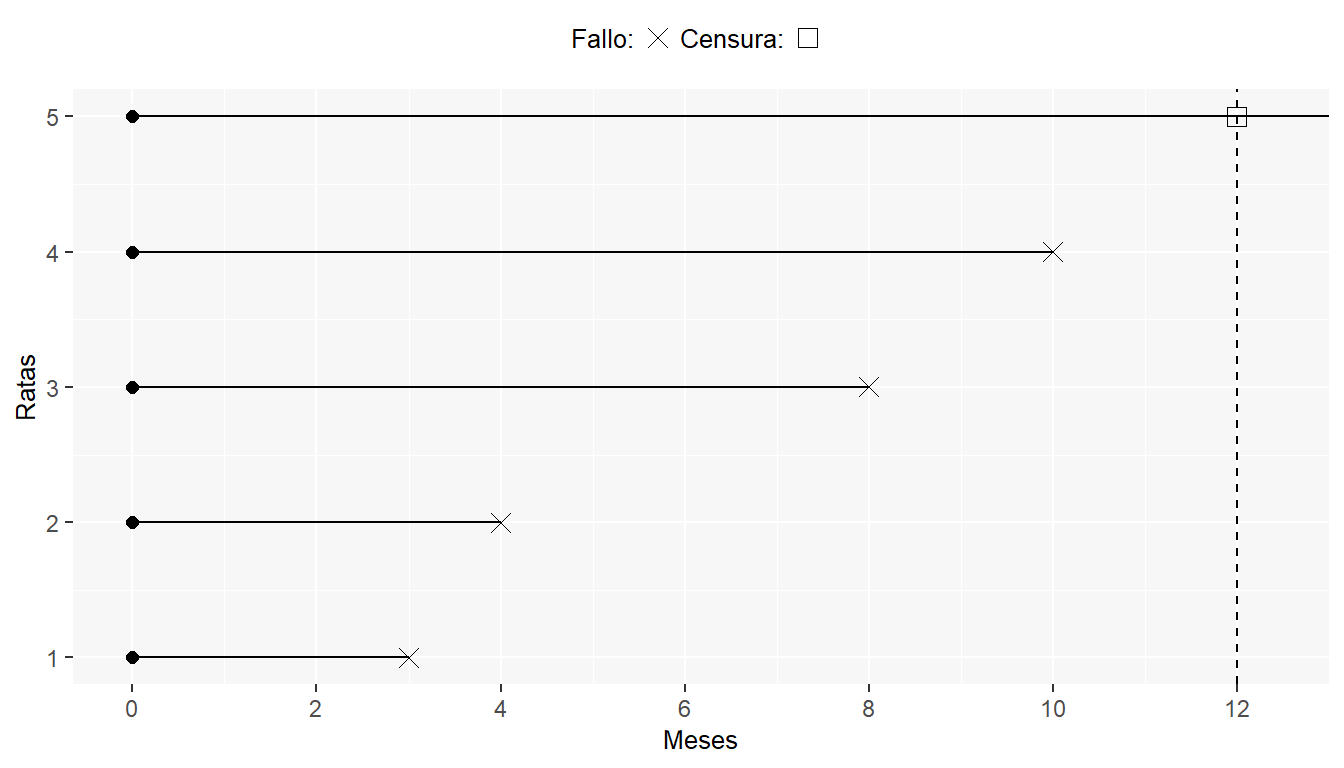
\includegraphics{_main_files/figure-latex/unnamed-chunk-8-1} \end{center}

\hypertarget{censura-por-la-derecha-tipo-ii}{%
\section{Censura por la Derecha Tipo II}\label{censura-por-la-derecha-tipo-ii}}

Ocurre cuando el estudio continua hasta que se presenta la falla de los primeros \(r<n\) individuos. Donde \(r\) es el número de individuos predeterminado a observar y \(n\) es el número total de individuos en el estudio. En este tipo de censura hay dependencia del tamaño de muestra y de las fallas que se observen.

\hypertarget{ejemplo-1}{%
\subsubsection*{Ejemplo}\label{ejemplo-1}}


Las limitaciones económicas para la investigación científica han hecho que un especialista en cancerología tome la decisión de observar los tiempos (en días) de sólo 5 conejos hasta que desarrollen un tumor, de un total de 9. Al final se obtuvo lo siguiente: \(30,34,43,45,60,60^+,60^+,60^+,60^+\), ¿Cómo interpretaría usted los resultados obtenidos por el especialista?

\begin{center}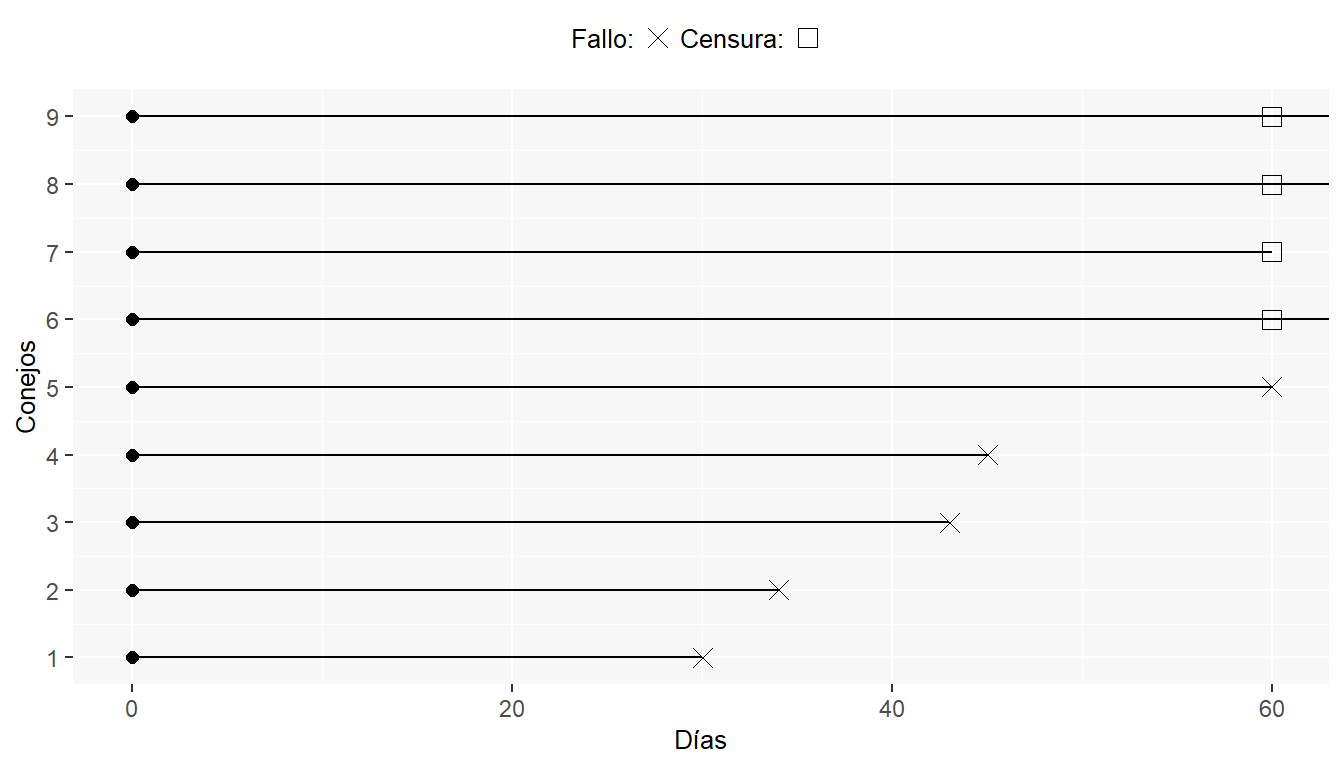
\includegraphics{_main_files/figure-latex/unnamed-chunk-9-1} \end{center}

\hypertarget{censura-por-la-derecha-tipo-iii}{%
\section{Censura por la Derecha Tipo III}\label{censura-por-la-derecha-tipo-iii}}

Llamada también censura aleatoria. Se denomina así porque el tiempo de censura lo determina un fenómeno aleatorio, que tiene lugar durante la consecución del estudio e impide seguir con la observación del individuo hasta el tiempo final; es decir que \(T_i\) es una variable aleatoria. En general, la censura aleatoria surge cuando los individuos salen del estudio sin presentar la falla por razones \textbf{no} controladas por el investigador. Cuando sucede tal censura, se dice que se tiene una \emph{análisis de riesgos competitivos}.

Finalmente, si el mecanismo de censura aleatoria es \emph{dependiente} de los tiempos de falla, se dice que este es una \emph{censura informativa}, ya que otorga información a los tiempos de falla; en caso contrario es \emph{no informativa}.

\hypertarget{ejemplo-2}{%
\subsubsection*{Ejemplo}\label{ejemplo-2}}


Algunos ejemplos son la migración a otra ciudad o los casos donde el paciente se retira del estudio o muere por alguna causa ajena al evento de interés. La siguiente gráfica muestra un ejemplo de datos con censura aleatoria.

\begin{center}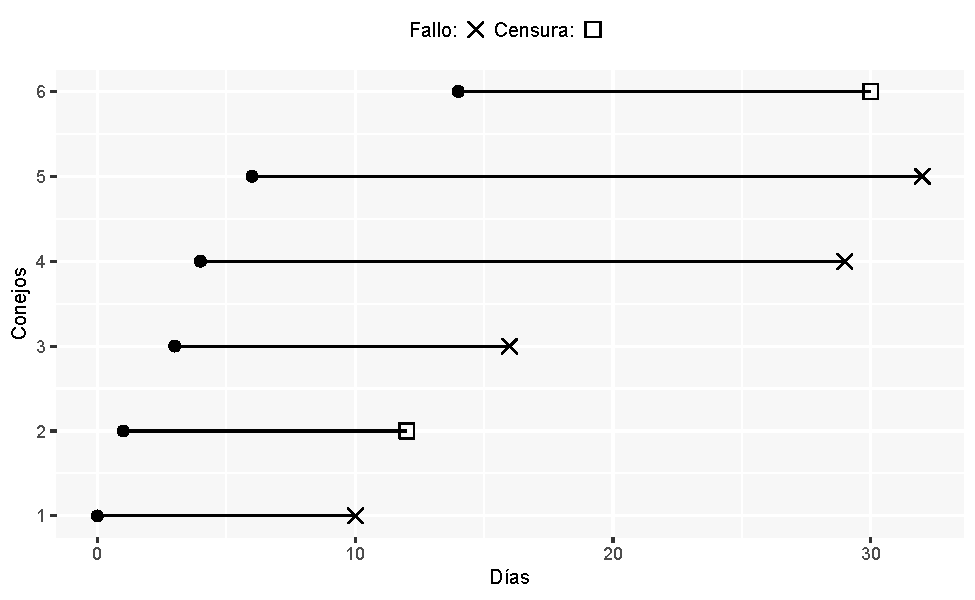
\includegraphics{_main_files/figure-latex/unnamed-chunk-10-1} \end{center}

\hypertarget{censura-por-la-izquierda}{%
\section{Censura por la Izquierda}\label{censura-por-la-izquierda}}

Las observaciones censuradas por la izquierda serán aquellas en las que el evento de interés ha tenido lugar antes del punto de inicio del estudio. Así, el tiempo de censura en este caso será el tiempo de inicio del estudio.

\hypertarget{ejemplo-3}{%
\subsubsection*{Ejemplo}\label{ejemplo-3}}


Un ejemplo de este tipo de censura son los tiempos al primer uso de marihuana. Como se observa en el ejemplo en la introducción de este capítulo, el levantamiento de la información se hace sobre alumnos de preparatoria y hay casos en los que el inicio del consumo es a una edad previa al levantamiento de los datos. Entonces aquellos jóvenes cuyo primer uso de marihuana es a una edad previa a la registrada en ese momento, serán consideradas como observaciones censuradas por la izquierda.

Frecuentemente si un estudio tiene censura por la izquierda, entonces se tendrá doble censura, por lo que se denota como \(C_i\) al tiempo antes del cual algunos individuos presentan el evento de interés y \(C_d\) al tiempo después del cual algunos de los individuos presentan el evento de interés.

\hypertarget{censura-por-intervalos}{%
\section{Censura por Intervalos}\label{censura-por-intervalos}}

Ocurre cuando los individuos en el estudio son monitoreados intermitentemente en momentos discretos de tiempo, de modo que, es posible que el suceso de estudio haya tenido lugar en un tiempo entre dos de las mediciones.

Si el individuo \(i\) no ha presentado el evento de interés al fin del tiempo \(I_i\) pero a la siguiente observación \(D_i\) sí presentó el evento, entonces es una falla censurada en el intervalo \((I_i,D_i)\).

\hypertarget{ejemplo-4}{%
\subsubsection*{Ejemplo}\label{ejemplo-4}}


Un investigador lleva a cabo un estudio en ratas diseñado para evaluar los efectos de dietas ricas en vegetales en el riesgo de cáncer de mama. El tumor mamario es inducido con una única dosis de DMBA al inicio del estudio. 6 semanas después de la administración del DMBA, cada rata es examinada una vez a la semana por 14 semanas y el tiempo en que el tumor es palpable es registrado. Si una rata presenta tumor en la quinta revisión, entonces lo que se sabe es que el tumor en la cuarta revisión no era palpable y por lo tanto este debió presentarse entre la cuarta y quinta revisión dando como resultado que esa observación esta censurada en el intervalo (semana 10, semana 11).

\hypertarget{datos-truncados}{%
\chapter{Datos Truncados}\label{datos-truncados}}

El truncamiento tiene lugar cuando sólo aquellos sujetos que manifiestan el evento dentro de una ventana observacional \((U,V)\) son observados, del resto no se realiza ningún seguimiento y, por tanto, no se obtiene información sobre ellos (no hay información parcial). Las observaciones \(t_i\) tales que \(t_i<U\), serán observaciones truncadas por la izquierda y aquellas que \(t_i>V\) serán observaciones truncadas por la derecha.

\hypertarget{ejemplos-de-datos-truncados}{%
\subsubsection*{Ejemplos de Datos Truncados}\label{ejemplos-de-datos-truncados}}


Deseamos medir la supervivencia de adultos mayores de 60 años. Entonces necesitamos que los individuos tengan al menos 60 años para que sean considerados en el estudio, por lo que el estudio está truncado por la izquierda. Otro ejemplo es si deseáramos medir la distancia de la tierra a las estrellas, este sería truncado por la derecha ya que no se puede ver más allá de un límite.

Es importante mencionar que la diferencia entre \emph{truncamiento} y \emph{censura} es la información parcial disponible. En datos censurados hay información parcial, mientras que en datos truncados no.

\hypertarget{ejemplos-del-caso-continuo-y-caso-discreto}{%
\subsubsection*{Ejemplos del caso continuo y caso discreto}\label{ejemplos-del-caso-continuo-y-caso-discreto}}


Un número grande de individuos sanos fueron enrolados en un estudio que inicio el 1/01/1970. Los individuos fueron seguidos por 30 años para estudiar la edad a la que desarrollaron cáncer de mama. Fueron sometidos a exámenes clínicos cada 3 años. Menciona si hay censura o truncamiento en:

\begin{enumerate}
\def\labelenumi{\arabic{enumi}.}
\tightlist
\item
  Individuo sano, enrolado a los 30 años, durante el periodo de estudio nunca desarrollo cáncer de mama.
\item
  Individuo sano, enrolado en el estudio con 40 años de edad, se le diagnosticó cáncer de mama en el quinto examen clínico.
\item
  Individuo sano, enrolado con 50 años de edad, murió a los 63 años por paro cardíaco.
\item
  Individuo con cáncer de piel en remisión.
\end{enumerate}

\hypertarget{ejercicios}{%
\section{Ejercicios}\label{ejercicios}}

\begin{enumerate}
\def\labelenumi{\arabic{enumi}.}
\tightlist
\item
  El análisis de supervivencia es un conjunto de procedimientos estadísticos para el cual la variable ``respuesta'' o de interés es dicotómica.
\end{enumerate}

\begin{enumerate}
\def\labelenumi{\alph{enumi}.}
\tightlist
\item
  Cierto, la variable que nos interesa es: ocurre la falla/evento o no
\item
  Falso, la variable de interés es ``tiempo hasta la ocurrencia del evento'' la cual es continua
\item
  El enunciado no tiene sentido, hay más de una variable de interés, por ejemplo: género, edad e incluso la distribución asociada.
\end{enumerate}

\begin{enumerate}
\def\labelenumi{\arabic{enumi}.}
\setcounter{enumi}{1}
\tightlist
\item
  Si un estudio termina antes de que un individuo desarrolle la falla, entonces su supervivencia está censurada.
\end{enumerate}

\begin{enumerate}
\def\labelenumi{\alph{enumi}.}
\tightlist
\item
  Cierto, se trata de una censura tipo I
\item
  Un estudio no puede terminar si no fallaron todos los individuos
\item
  Falso, es truncada porque t \textless{} U, donde t es el tiempo del estudio y U es el tiempo de falla
\item
  No se puede concluir, hace falta conocer las características estudio
\end{enumerate}

\begin{enumerate}
\def\labelenumi{\arabic{enumi}.}
\setcounter{enumi}{2}
\tightlist
\item
  Una empresa encargada del transporte de frutas via mar ́ıtima a mercados internacionales desea medir el tiempo de maduración de los aguacates para poder asegurar que estos lleguen en ́optimo estado a su destino. La empresa tiene 3 diferentes propuestas para realizar este estudio. Se deben analizar las tres propuestas en función del tipo de censura y/o truncamiento que presentar ́an los datos recolectados para con ello escoger la mejor propuesta.
\end{enumerate}

\begin{enumerate}
\def\labelenumi{\alph{enumi}.}
\tightlist
\item
  El estudio 1 propone tomar la medición inicial del nivel de maduración en el momento en que se cargan los aguacates en el barco y una segunda medición al llegar al puerto de destino
\item
  El estudio 2 propone tomar la medición inicial del nivel de maduración en el momento de corte de la fruta con los agricultores, una segunda medición al entrar en la cámara de refrigeración en el barco, después tomar mediciones cada cinco dias hasta llegar al destino, en donde se toma una medición final
\item
  El estudio 3 propone replicar las condiciones del transporte en una cámara frigorífica en el puerto de salida. Al llegar los aguacates al puerto se relaiza una selección de los 1000 menos maduros, estos se introducen en el frigorífico y se tomarán mediciones de la maduración diario por un periódo de 30 dias.
  Después de analizar las propuestas, diga que estudio propondría a la empresa llevar a cabo y por que.
\end{enumerate}

\hypertarget{part-estudio-paramuxe9trico}{%
\part{Estudio paramétrico}\label{part-estudio-paramuxe9trico}}

\hypertarget{funciones-para-el-anuxe1lisis-de-supervivencia}{%
\chapter{Funciones para el Análisis de Supervivencia}\label{funciones-para-el-anuxe1lisis-de-supervivencia}}

Dado que el análisis de supervivencia se basa en tiempos de falla, definiremos a continuación funciones importantes que se pueden asociar a estos. Evidentemente, estamos pensando que los tiempos de falla provienen de una variable aleatoria \textbf{No negativa}\footnote{Véase que al mencionar que la variable \(T\) es no negativa se da por entendido que dicha variable aleatoria en el espacio de probabilidad \((\Omega, S, \mathbb{P})\), donde \(\Omega\) es el espacio muestral, \(S\) la \(\sigma\)-álgebra definida en \(\Omega\) y \(\mathbb{P}\) la medida de probabilidad correspondiente, asigna valores en \(\mathbb{R}^{+\{0\}}\); es decir: \(T:\Omega\rightarrow\mathbb{R}^{+\{0\}}\).} \(T\) la cual llamaremos \emph{variable aleatoria del tiempo de falla}, equivalentemente \emph{longitud de tiempo de vida futura} o \emph{tiempo de superviviencia}. Por simplicidad la llamaremos \emph{tiempo de supervivencia}.

\(T\) es usualmente descrita o caracterizada por cuatro funciones:

\begin{itemize}
\tightlist
\item
  \emph{1.- Función de supervivencia}
\item
  \emph{2.- Función de densidad de probabilidad}
\item
  \emph{3.- Función de riesgo}
\item
  \emph{4.- Función de riesgo acumulado}
\end{itemize}

Estas funciones son matemáticamente equivalentes; a partir de una se derivan las otras tres. Cabe destacar que, dependiendo el caso, \(T\) puede ser una variable aleatoria continua o bien, discreta.

\hypertarget{funciuxf3n-de-supervivencia}{%
\section{Función de Supervivencia}\label{funciuxf3n-de-supervivencia}}

\hypertarget{caso-continuo}{%
\subsection*{Caso continuo}\label{caso-continuo}}


La función de supervivencia \(S(t)\), tanto en el caso continuo como en el discreto, se define como la probabilidad de que un individuo sobreviva más allá del tiempo \(t\). Para el caso continuo:

\[
S(t)=\mathbb{P}(T>t)=1-F_T(t)=\int_{t}^{\infty}f_T(u)du
\]

Si tomamos la igualdad \(S(t)=1-F_T(t)\) y derivamos en ambos lados y multiplicamos por \(-1\), obtenemos:

\[
-\frac{d}{dt}S(t)=f_T(t)
\]

Las propiedades de \(S(t)\) son:

1.-Es monótona no creciente.

2.- \(S(t)=1\) para \(t=0\).

3.- \(S(t)=0\) cuando \(t\rightarrow\infty\).

La función \(S(t)\) es conocida también como la \emph{tasa de superviviencia acumulativa}; en el contexto industrial se conoce como \emph{función de confiabilidad}.

Por otro lado, es de suma importancia representar \(S(t)\) gráficamente ya que de ella se puede obtener información interesante; por ejemplo el cálculo de diversos cuantiles (como el cuantil 50) nos permitirán hacer inferencias y comparar distribuciones de superviviencia de dos o más grupos de individuos. La gráfica de \(S(t)\) es llamada \textbf{curva de supervivencia}, los gráficos de la figura \ref{fig:two-example-survival-functions} son ejemplos de esta.

\begin{figure}

{\centering 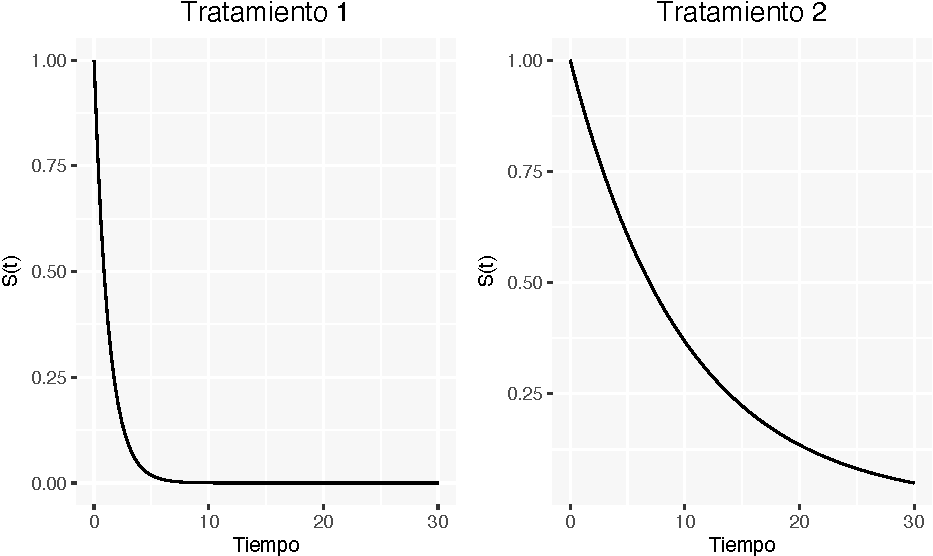
\includegraphics{_main_files/figure-latex/two-example-survival-functions-1} 

}

\caption{Ejemplos de la curva de supervivencia.}\label{fig:two-example-survival-functions}
\end{figure}

En la primer gráfica se observa una tasa de supervivencia baja, mientras que en la segunda gráfica se tiene una tasa alta. En este contexto, ¿qué podríamos decir de los pacientes con el tratamiento 1 \emph{versus} los pacientes con el tratamiento 2?

\hypertarget{caso-discreto}{%
\subsection*{Caso discreto}\label{caso-discreto}}


Si \(T\) es una variable aleatoria discreta que toma valores \(0<t_1<t_2<...\) Entonces la función de probabilidad de \(T\) es:

\[
f(t) = \left\{
\begin{array}{ll}
\mathbb{P}(T=t_j) & \mbox{ si  } t=t_j, j=1,2,...\\
0 & \mbox{en otro caso }
\end{array}
\right.
\]

Por lo que su función de supervivencia es:

\[
S(t)=\mathbb{P}(T> t)=\sum_{t< t_j}f(t_j)
\]
La siguiente es una representación gráfica de la función de supervivencia en el caso discreto

\begin{center}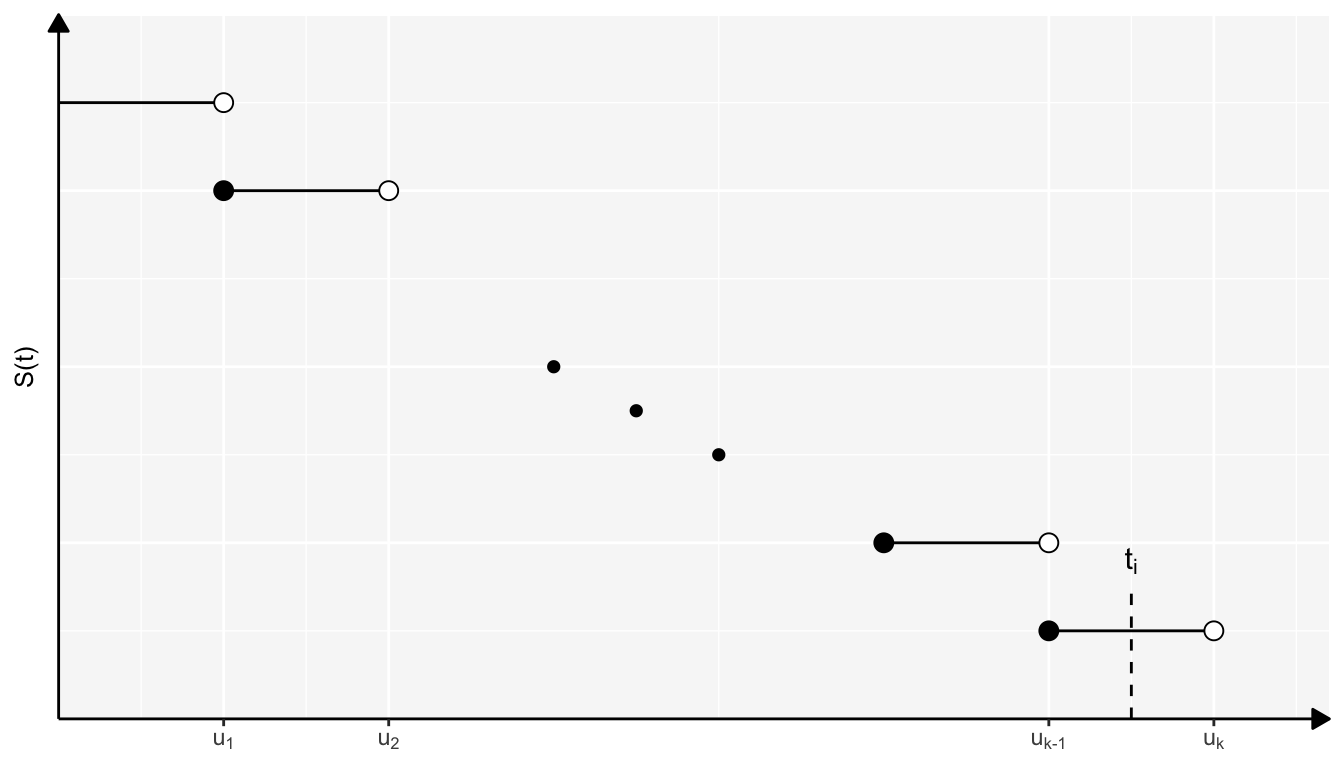
\includegraphics{_main_files/figure-latex/unnamed-chunk-11-1} \end{center}

Al igual que el caso continuo, se tienen las propiedades:

1.-Es monótona no creciente

2.- \(S(t)=1\) para \(t=0\).

3.- \(S(t)=0\) cuando \(t\rightarrow\infty\).

\hypertarget{ejemplos-del-caso-continuo-y-caso-discreto-1}{%
\subsubsection*{Ejemplos del caso continuo y caso discreto}\label{ejemplos-del-caso-continuo-y-caso-discreto-1}}


Estos pueden verse al final de la sección \ref{par-poblacionales}

\hypertarget{RiskFunction}{%
\section{Función de Riesgo}\label{RiskFunction}}

\hypertarget{caso-continuo-1}{%
\subsection*{Caso continuo}\label{caso-continuo-1}}


La función de riesgo \(h(t)\) (hazard function), también llamada \textbf{tasa de falla condicional} (en el análisis de confiabilidad) o \emph{tasa de mortalidad} (en demografía), se define como la probabilidad de falla durante un intervalo de tiempo muy pequeño suponiendo que el individuo ha sobrevivido hasta el inicio del intervalo\footnote{Aunque en la definición de \(h(t)\) se tenga explícitamente la palabra ``probabilidad'', hay que tener en claro que esta función no es una función de probabilidad, si no tal cual una \textbf{tasa}, ya que la acumulación de esta puede dar valores superiores a 1.}; en expresiones matemáticas es:

\[
h(t)=\lim_{\alpha\rightarrow 0}\frac{1}{\alpha}\mathbb{P}(t<T\leq t+\alpha|T\geq t)
\\
=\lim_{\alpha\rightarrow 0}\frac{1}{\alpha}\frac{\mathbb{P}(T\leq t+\alpha)-\mathbb{P}(T<t)}{\mathbb{P}(T\geq t)}\\
=\lim_{\alpha\rightarrow 0}\frac{1}{\alpha}\frac{F(t+\alpha)-F(t)}{S(t)}
=\frac{f(t)}{S(t)}
\]

Entonces

\[
h(t)=\frac{f(t)}{S(t)}=\frac{f(t)}{1-F(t)}=-\frac{d}{dt}log(S(t))
\]

Si tomamos la igualdad

\[
h(t)=-\frac{d}{dt}log(S(t))
\]

Y despejamos a \(S(t)\) tenemos que:

\[
S(t)=exp\left[-\int_{0}^{t}h(u)du\right]=exp[-H(t)]
\]

Donde \(H(t)=\int_{0}^{t}h(u)du\) es conocida como \textbf{la función acumulada de riesgo}, la cual veremos más adelante.

La función de riesgo juega un papel importante en el análisis de supervivencia. Describe la forma en que cambia la \emph{tasa instantánea de muerte de un individuo al paso del tiempo} (constante, lineal, exponencial, etc.). El conocer \(h(t)\) puede darnos alguna idea sobre la selección del modelo para la distribución del tiempo de supervivencia, por ejemplo, puede ser útil al considerar restricciones para modelos con funciones de riesgo no decrecientes o modelos con funciones de riesgo no crecientes.

No hay un comportamiento ``habitual'' en la gráfica de \(h(t)\), es decir, \(h(t)\) puede crecer, decrecer, ser constante o mostrar algo más complicado. El esquema siguiente muestra algunos ejemplos de la gráfica de \(h(t)\):

\begin{center}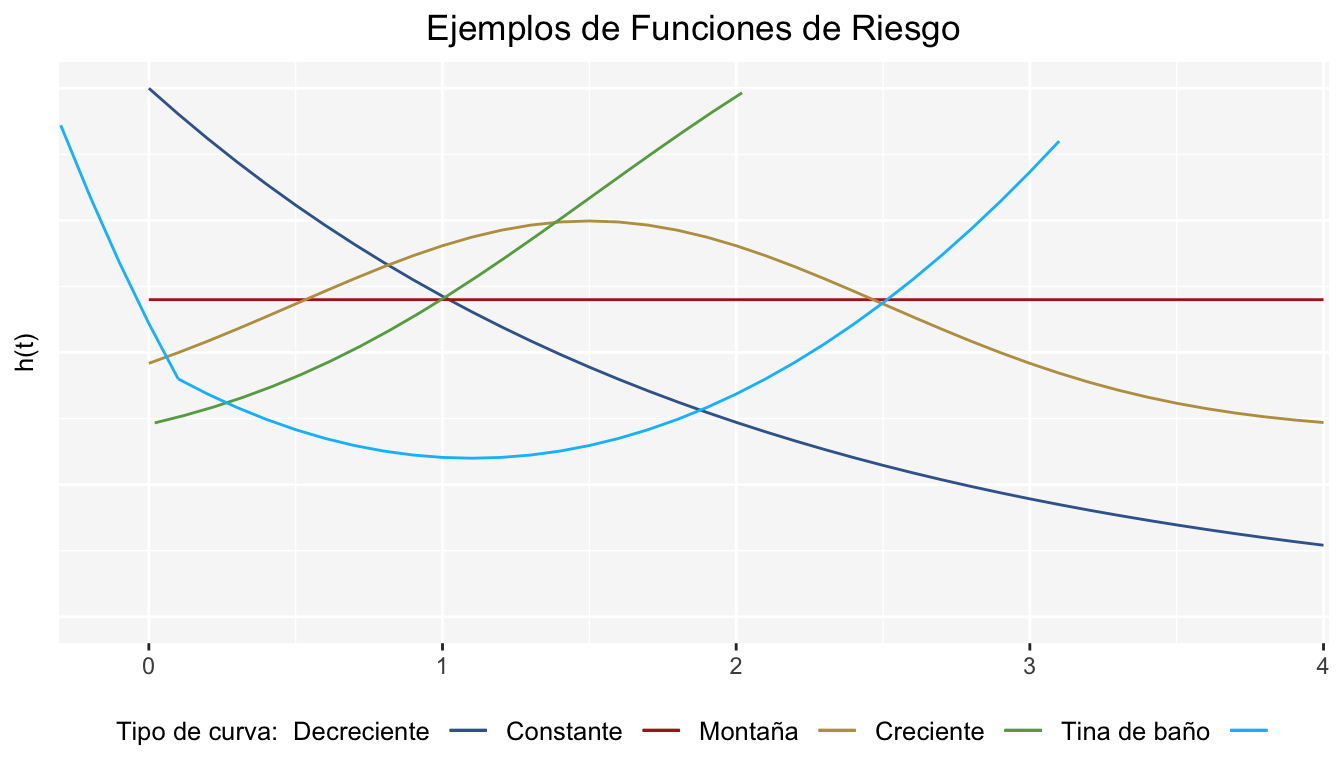
\includegraphics{_main_files/figure-latex/unnamed-chunk-12-1} \end{center}

La curva \(h(t)\) en color azul (\emph{llamada curva de tina de baño}) describe el proceso de la vida humana: al inicio existe mortalidad infantil y el riesgo de morir es alto, crece el individuo y el riesgo de morir se reduce y hasta cierto punto es constante, después viene el envejecimiento(hay deterioro) y entonces el riesgo de morir aumenta. Una función de riesgo creciente como la curva de color verde implica un envejecimiento natural. Una función decreciente como la curva color morado es menos común e indica rejuvenecimiento. Una función en forma de montaña como la curva color café, podría representar un comportamiento de muerte por enfermedad después de llevar un tratamiento para la misma enfermedad.

\hypertarget{caso-discreto-1}{%
\subsection*{Caso discreto}\label{caso-discreto-1}}


En este caso, la función de riesgo proporciona la probabilidad condicional de falla al tiempo \(t=u_k\), dado que el individuo estaba vivo antes de \(u_k\).

Sea \(T\) una variable aleatoria discreta con soporte en \(\{u_1,u_2,u_3,...\}\). La función de riesgo al tiempo \(u_k\) se define como\footnote{\(\mathbb{P}(T\geq u_k) = \mathbb{P}(T>u_{k-1}) = S(u_{k-1})\) por el hecho de estar tratando con una variable discreta, ya que el siguiente valor de \(u_{k-1}\) en la lista \(\{u_1, \dots, u_{k-1}, u_{k}\}\) es \(u_k\). Además, véase que el uso de \(f_T(u_k)\) en este caso discreto es simplemente notación y no se debe confundir con la función de densidad de la v.a \(T\).}

\[
h(u_k)=\mathbb{P}(T=u_k|T\geq u_k)=\frac{\mathbb{P}(T=u_k)}{\mathbb{P}(T\geq u_k)} =\frac{f_T(u_k)}{S_T(u_{k-1})}
\]

Observemos que:

\[
f_T(u_k)=\mathbb{P}(T=u_k)=\mathbb{P}(T\geq u_k)-\mathbb{P}(T> u_{k})= S(u_{k-1})-S(u_{k})
\]

si dividimos entre \(S(u_{k-1})\), tenemos entonces:

\[
h(u_k)=\frac{S(u_{k-1})-S(u_{k})}{S(u_{k-1})}=1-\frac{S(u_{k})}{S(u_{k-1})}
\]

Por otro lado, para \(S(t)\) se cumple que:

\[
S(t)=\frac{S(t)}{1}=\frac{S(t)}{S(0)}=\frac{S(u_1)}{S(0)}.\frac{S(u_2)}{S(u_1)}.\frac{S(u_3)}{S(u_2)}...\frac{S(u_k)}{S(u_{k-1})}.\frac{S(t)}{S(u_k)}
\]

Entonces, de la expresión anterior y ocupando que \(h(u_k)=1-\frac{S(u_{k})}{S(u_{k-1})}\) tenemos finalmente:

\[
S(t)=\prod_{k: u_k \leq t}\frac{S(u_k)}{S(u_{k-1})} =\prod_{k: u_k \leq t}(1-h(u_k))
\]

Si queremos obtener \(f(u_k)\), la podemos conocer partir de la función de riesgo:

\[
f(u_k)=\frac{f(u_k)}{S(u_{k-1})}S(u_{k-1})=h(u_k)S(u_{k-1})=h(u_k) \prod_{j<k} \frac{S(u_j)}{S(u_{j-1})}=h(u_k) \prod_{j<k}(1-h(u_j))
\]

La expresión

\[
S(t)=\prod_{k: u_k \leq t}(1-h(u_k))
\]

la ocuparemos más adelante.

\hypertarget{ejemplo-5}{%
\subsubsection*{Ejemplo}\label{ejemplo-5}}


Suponga que se tiene la siguiente distribución para la variable aleatoria \(T\): \(\mathbb{P}(T = j) = \frac{1}{3}; \ \ j = 1,2,3\)

Para este caso se tienen los siguientes resultados junto con las siguientes representaciones gráficas:

\[
S(t) = \left\{
\begin{array}{ll}
1 & -\infty<t<1\\
\frac{2}{3} &  1\leq t<2\\
\frac{1}{3} & 2\leq t < 3\\
0 & t\geq 3
\end{array}
\right.
h(t) = \left\{
\begin{array}{ll}
\frac{f(1)}{S(0)} = \frac{1}{3} & t = 1\\
\frac{f(2)}{S(1)} = \frac{1}{2} & t = 2\\
\frac{f(3)}{S(2)} = 1 & t = 3
\end{array}
\right.
\]

\begin{center}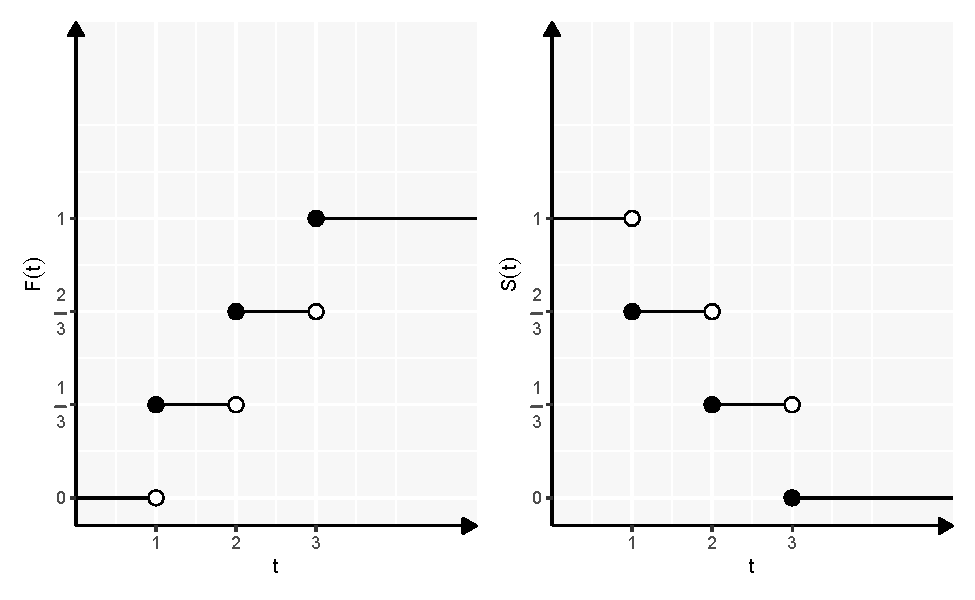
\includegraphics{_main_files/figure-latex/unnamed-chunk-13-1} \end{center}

\hypertarget{funciuxf3n-de-riesgo-acumulado}{%
\section{Función de Riesgo Acumulado}\label{funciuxf3n-de-riesgo-acumulado}}

\hypertarget{caso-continuo-2}{%
\subsection*{Caso continuo}\label{caso-continuo-2}}


Esta función, denotada por \(H(t)\), es importante en la medición de la frecuencia con que ocurren los fallos en el tiempo y en el análisis de residuos para el ajuste de algunos modelos. \(H(t)\) se define como sigue:

\[
H(t)=\int_{0}^{t}h(u)du
\]
Hemos visto anteriormente que:

\[
S(t)=exp(-H(t))
\]

entonces

\[
H(t)=-log(S(t))
\]

Podemos calcular a \(f(t)\) en términos de \(h(t)\) y \(H(t)\):

\[
f(t)=h(t)S(t)=h(t)exp(-H(t))
\]

\hypertarget{caso-discreto-2}{%
\subsection*{Caso discreto}\label{caso-discreto-2}}


\(H(t)\) se define como:

\[
H(t)=\sum_{k: u_k\leq t}h(u_k)
\]

Una definición alternativa es:

\[
H(t)=-\sum_{k: u_k\leq t}log(1-h(u_k))
\]

\hypertarget{par-poblacionales}{%
\chapter{Parámetros Poblacionales}\label{par-poblacionales}}

Si conocemos la distribución de \(T\) (cuando sea posible) es importante extraer cierta información que nos ayude a sacar conclusiones sobre los tiempos de supervivencia; a saber, información sobre su(s) parámetro(s). Aunque es habitual pensar a \(T\) como una variable aleatoria continua, a continuación presentaremos parámetros poblacionales en términos de la función de superviviencia para el caso continuo y discreto.

\hypertarget{media}{%
\section{Media}\label{media}}

\hypertarget{caso-continuo-3}{%
\subsection*{Caso continuo}\label{caso-continuo-3}}


Para el caso continuo se tiene:

\[
\mu=\mathbb{E}[T]=\int_{0}^{\infty}\mathbb{P}(T>t)=\int_{0}^{\infty}S(t)dt
\]

La demostración se queda como ejercicio al alumno.

\hypertarget{caso-discreto-3}{%
\subsection*{Caso discreto}\label{caso-discreto-3}}


\(\mu\) en este caso es de la forma:

\[
\mu=\mathbb{E}[T]=\sum_{k=1}^{\infty}u_kf(u_k)=\sum_{k=1}^{\infty}S(u_k)
\]

La demostración se queda como ejercicio al alumno.

\hypertarget{varianza}{%
\section{Varianza}\label{varianza}}

\hypertarget{caso-continuo-4}{%
\subsection*{Caso continuo}\label{caso-continuo-4}}


Para este caso la varianza se ve como:

\[
  \sigma^2=Var[T]=\mathbb{E}[T^2]-(\mathbb{E}[T])^2=2\int_{0}^{\infty}tS(t)dt-\left(\int_{0}^{\infty}S(t)dt\right)^2
\]

La demostración de la igualdad anterior se obtiene si se observa que:

\[
\mathbb{E}[T^2]=\int_{0}^{\infty}t^2f(t)dt=-t^2S(t)|_0^{\infty}+2\int_{0}^{\infty}tS(t)dt=2\int_{0}^{\infty}tS(t)dt
\]

Y ocupando que:

\[
\mathbb{E}[T]=\int_{0}^{\infty}S(t)dt
\]

\hypertarget{caso-discreto-4}{%
\subsection*{Caso discreto}\label{caso-discreto-4}}


De manera similar:

\[
  \sigma^2=Var[T]=\mathbb{E}[T^2]-(\mathbb{E}[T])^2=2\sum_{k=1}^{\infty}u_kS(u_k)-\left(\sum_{k=1}^{\infty}S(u_k)\right)^2
\]

La demostración se queda de ejercicio al alumno.

\hypertarget{funciuxf3n-de-media-residual}{%
\section{Función de Media Residual}\label{funciuxf3n-de-media-residual}}

Para individuos de edad \(x\) este parámetro, denotado por \(mr(x)\), mide la esperanza de vida residual; esto es, ``la esperanza de vida que les queda a partir de la edad \(x\)''.

\hypertarget{caso-continuo-5}{%
\subsection*{Caso continuo}\label{caso-continuo-5}}


Se define como:

\[
mr(x)=\mathbb{E}[T-x|T>x]=\frac{\mathbb{E}[T-x]}{\mathbb{P}(T>x)}=\frac{\int_x^{\infty}(t-x)f(t)dt}{S(x)}=\frac{\int_x^{\infty}S(t)dt}{S(x)}
\]

\hypertarget{caso-discreto-5}{%
\subsection*{Caso discreto}\label{caso-discreto-5}}


Para este caso es:

\[
mr(u_x)=\frac{\sum_{k=x}^{\infty}S(u_k)}{S(u_x)}
\]

\hypertarget{cuantiles-de-orden-p}{%
\section{\texorpdfstring{Cuantiles de Orden \(p\)}{Cuantiles de Orden p}}\label{cuantiles-de-orden-p}}

El cálculo de diversos cuantiles nos permitirá hacer comparaciones entre diversos grupos de sujetos, además de obtener información sobre los tiempos de falla, por ejemplo, el tiempo mediano de falla (a veces es mejor el cálculo de la mediana que la media).

\hypertarget{caso-continuo-6}{%
\subsection*{Caso continuo}\label{caso-continuo-6}}


El cuantil o percentil, \(t_p\), de orden \(p\) de la variable aleatoria continua \(T\) será aquel que:

\[
S(t_p)=1-p
\]

Si queremos el tiempo mediano de los tiempos de supervivencia entonces debemos calcular \(t_{0.5}\) talque:

\[
S(t_{0.5})=0.5
\]

\hypertarget{caso-discreto-6}{%
\subsection*{Caso discreto}\label{caso-discreto-6}}


En este caso \(t_p\) es:
\[
t_p=inf\{t: S(t) \leq  1-p\}
\]

\hypertarget{ejemplo-1-1}{%
\subsubsection*{Ejemplo 1}\label{ejemplo-1-1}}


Siguiendo el ejemplo presentado en la sección \ref{RiskFunction}, se tiene lo siguiente:

\begin{itemize}
\tightlist
\item
  Función de supervivencia de \(T\): \(S(t) = \mathbb{P}(T>t)=\left\{\begin{array}{ll}1 & \mbox{si }t=1\\\frac{2}{3} & \mbox{si } t=2\\\frac{1}{3} & \mbox{si } t = 3\\0 & \mbox{si }t>3\end{array}\right.\)
\item
  Función de riesgo: \(h(t) =\left\{\begin{array}{ll}\frac{1}{3} & \mbox{si }t=1\\\frac{1}{2} & \mbox{si } t=2\\\ 1 & \mbox{si } t = 3\end{array}\right.\)
\item
  \(\mu = \mathbb{E}(T) = \sum\limits_{t = 1}^3S(t) = \sum\limits_{t = 1}^3t\cdot f(t) = 2\).
\item
  \(mrl(2) = \frac{\sum\limits_{k = 2}^\infty S(u_k)}{S(2)} = \frac{2/3+1/3+0}{2/3} = \frac{3}{2} = 1.5\).
\item
  \(t_{0.75} = inf\{t: S(t) \leq 0.15\} = 3\)
\end{itemize}

Con la finalidad de aclarar la distribución de los cuantiles en una distribución discreta, se dejan las siguientes gráficas correspondientes a este ejercicio.

\begin{center}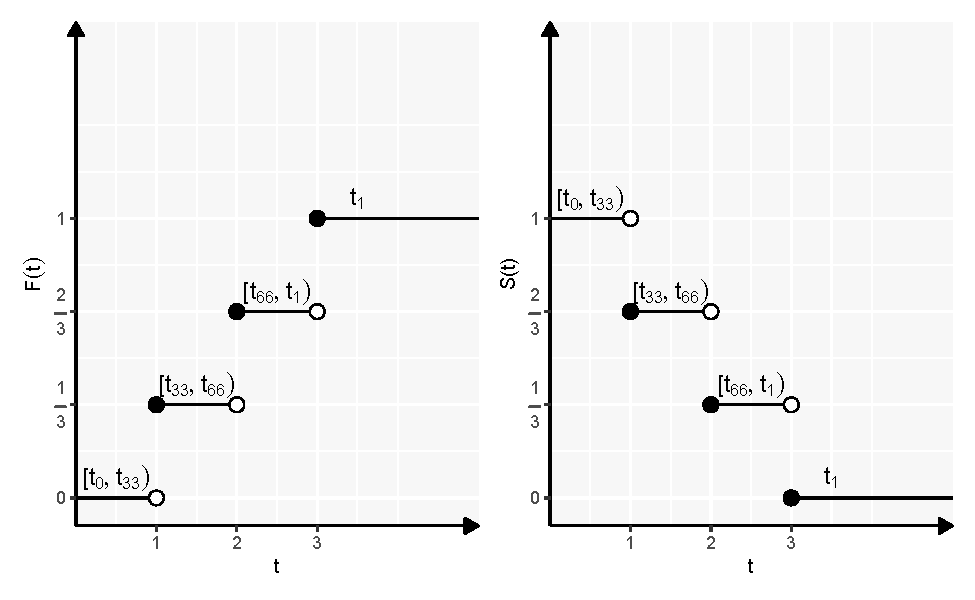
\includegraphics{_main_files/figure-latex/unnamed-chunk-14-1} \end{center}

\hypertarget{ejemplo-2-1}{%
\subsubsection*{Ejemplo 2}\label{ejemplo-2-1}}


Sea \(T\) una v.a con distribución uniforme continua en \((0,100)\) unidades días.

\begin{enumerate}
\def\labelenumi{\arabic{enumi}.}
\tightlist
\item
  Encontrar la función de supervivencia y evaluar la supervivencia para 30 y 35 años.
\item
  Encontrar la función de riesgo y evaluar el riesgo para 60 días.
\item
  Encontrar la esperanza de riesgo residual a los 75 días.
\end{enumerate}

Soluciones:

\begin{enumerate}
\def\labelenumi{\arabic{enumi}.}
\tightlist
\item
  \[
  f_T(t) = \left\{
  \begin{array}{ll}
  \frac{1}{100} & \forall\ \ t\in [0,100]\\
  0 & e.o.c
  \end{array}
  \right.
  \implies S(t) = 1-\int_0^t\frac{1}{100}dv = 1-\frac{t}{100}
  \]
  \[
  \implies S(30) = \mathbb{P}(T>30) = 1-\frac{30}{100};\ \  S(35) = 1- \frac{35}{100}
  \]
\item
  \[
  h(t) = \frac{f(t)}{S(t)} = \frac{\frac{1}{100}}{1-\frac{1}{100}} = \frac{1}{100-t}\\
  \implies h(60) = \frac{1}{100-60} = \frac{1}{40}
  \]
\item
  \[
  mrl(x) = \mathbb{E}(T-75 | T>75) = \frac{\mathbb{E}(T-75)}{\mathbb{P}(T>75)} = \frac{\int_x^\infty(t-75)f(t)dt}{S(75)} = \frac{\int_x^{100}(t-75)\frac{1}{100}dt}{1-\frac{75}{100}}
  \]
  \[
  \implies mrl(75) = \frac{1}{25}\int_{75}^{100}(t-75)dt = \frac{1}{25}\left(\frac{100^2}{2}-\frac{75^2}{2}\right)-\frac{75(100-75)}{25} = \frac{25}{2} = 12.5
  \]
  Otra solución
\end{enumerate}

Demostrandose que \(\int_x^\infty(t-x)f(t) dt = \int_x^\infty S(t)dt\)

\[
\implies mrl(75) = \frac{\int_{75}^{100}(t-75)\frac{1}{100}dt}{S(75)} = \frac{\int_{75}^{100}S(75)dt}{S(75)} = 12.5
\]

\hypertarget{modelos-paramuxe9tricos}{%
\chapter{Modelos Paramétricos}\label{modelos-paramuxe9tricos}}

Existen varios modelos paramétricos que se emplean en el análisis de supervivencia, esto se debe a que pueden representar de manera adecuada el comportamiento de ciertos fenómenos. La motivación para usar un modelo en particular es, por lo general, empírica; o bien, con base en la información que proporcione algún modelo \textbf{No paramétrico}. Las familias paramétricas más importantes son: \emph{Exponencial, Weibull, Log-Normal, Log-logística} y \emph{Gamma}.

\hypertarget{modelo-exponencial}{%
\section{Modelo Exponencial}\label{modelo-exponencial}}

El modelo exponencial es el más importante debido a su amplia aplicación, por ejemplo, puede emplearse en estudios para determinar el tiempo de vida útil de algunos artículos manufacturados. Este modelo juega un papel fundamental análogo a la \emph{distribución normal} en la inferencia estadística tradicional.

\textbf{Función de Densidad}

\[
f(t)=h(t)S(t)=\lambda exp(-\lambda t)=\lambda e^{-\lambda t}
\]
Para esta distribución \(\lambda\) es un parámetro que modifica la escala de la distribución. Este es comúnmente llamado \textbf{\emph{tasa}} definido por \(1/s\) donde \(s\) es el verdadero parámetro de escala\footnote{Un parámetro de escala modifica la escala o \emph{dispersión} de la distribución ya sea que entre mayor sea este parámetro mayor dispersión se tendrá o se tenga el caso contrario como en una \emph{log-logistica}. En el siguiente \href{https://en.wikipedia.org/wiki/Scale_parameter}{enlace} se puede encontrar mayor información sobre esto así como animaciones para un mejor entendimiento.} de la distribución. Es muy común utilizar este parámetro en lugar del parámetro de escala ya que simplifica la expresión matemática.

\textbf{Función de Supervivencia}

\[
S(t)=exp\left(-\int_0^{t}h(u)du\right)=exp\left(-\int_0^{t}\lambda du\right)=exp(-\lambda t)=e^{-\lambda t}
\]

Si asumimos \textbf{una tasa de riesgo invariante en el tiempo}, \(h(t)=\lambda\) con \(\lambda>0\), generamos el modelo exponencial:

\textbf{Función de Riesgo}

Tomamos \(\lambda>0\) y hacemos:

\[
h(t)=\lambda
\]

Aunque el supuesto de una función de riesgo constante resulta ser una restricción considerable, el modelo exponencial no deja de ser útil e importante en variedad de aplicaciones. Cabe destacar, que este modelo cumple con la propiedad de \emph{pérdida de memoria}; a saber, se cumple que:

\[
\mathbb{P}(T>t+x|T>t)=\mathbb{P}(T>x)
\]

\textbf{Parámetros}

Si \(T\sim Exp(\lambda)\) entonces:

\[
\mathbb{E}[T]=\int_{0}^{\infty}t\lambda e^{-\lambda t}dt=\frac{1}{\lambda}
\]

Y

\[
Var[T]=\mathbb{E}[T^2]-\mathbb{E}[T]^2=\frac{2}{\lambda^2}-\frac{1}{\lambda^2}=\frac{1}{\lambda^2}
\]

\textbf{Gráficas}

A continuación se muestran gráficas de una \(Exponencial\) con \(\lambda=0.5\)

\begin{center}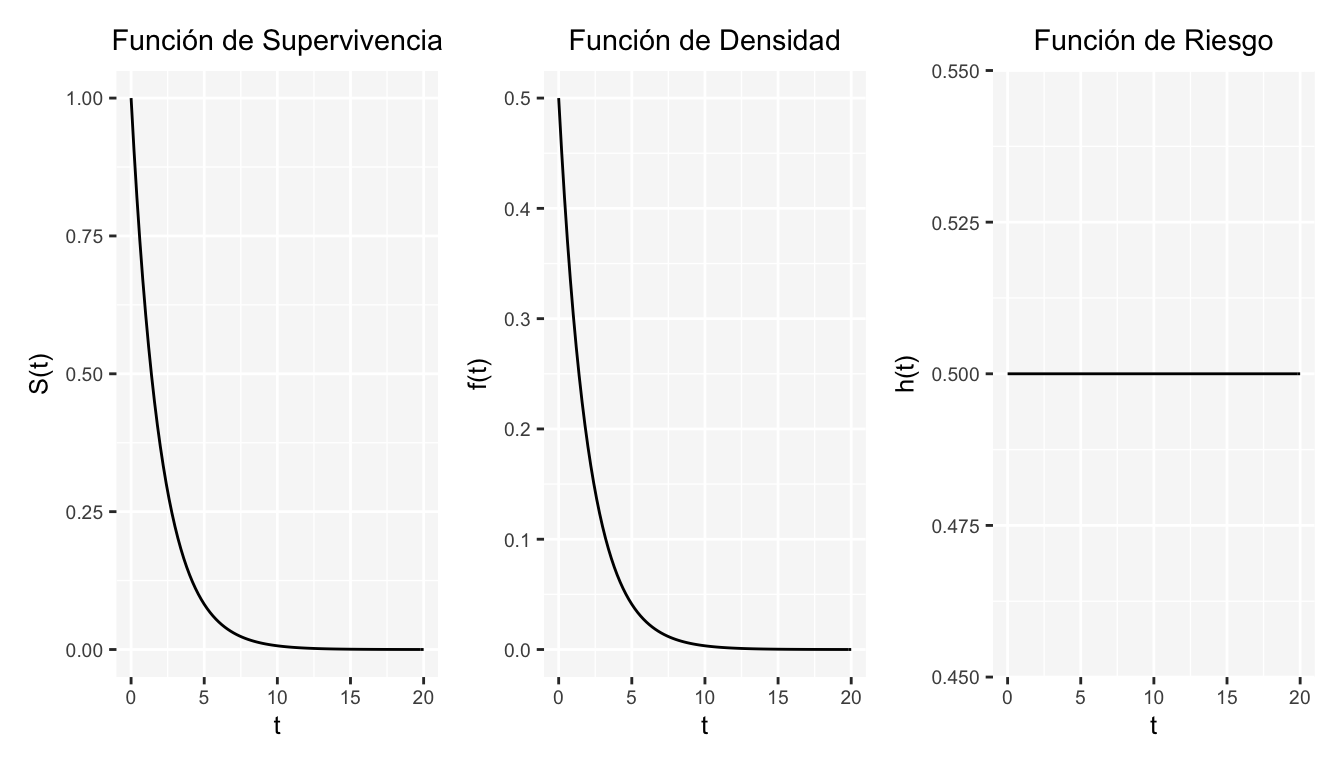
\includegraphics{_main_files/figure-latex/unnamed-chunk-15-1} \end{center}

\textbf{R}

En el lenguaje de programación \texttt{R} se pueden obtener resultados de esta distribución como una muestra pseudo aleatoria y aproximaciones numéricas para la distribución y densidad de esta así como la obtención de los cuantiles.

En general, el sufijo para esta distribución es \texttt{*exp}, de tal manera que se tienen las siguientes funciones mencionando la interpretación de sus resultados:

\begin{itemize}
\tightlist
\item
  \texttt{rexp(n,\ rate\ =\ 1)}: Muestra pseudo aleatoria de tamaño \(n\).
\item
  \texttt{dexp(x,\ rate\ =\ 1,\ log\ =\ FALSE)}: Valores de \(f(x)\).
\item
  \texttt{pexp(q,\ rate\ =\ 1,\ lower.tail\ =\ TRUE,\ log.p\ =\ FALSE)}: Valores de \(F(x)\).
\item
  \texttt{qexp(p,\ rate\ =\ 1,\ lower.tail\ =\ TRUE,\ log.p\ =\ FALSE)}: Cuantil \(t_p\).
\end{itemize}

Algo que hay que recordar es que al utilizar la función, por ejemplo, \texttt{rexp(n,\ r)} se respeta el orden de los parámetros por lo que \texttt{r} será el valor correspondiente a la tasa y no parámetro de escala es decir el valor \(r = \lambda\). Se menciona esta por que puede ser común que se confunda \texttt{r} con \(1/\lambda\), por lo que se recomienda tener precaución.

\hypertarget{modelo-weibull}{%
\section{Modelo Weibull}\label{modelo-weibull}}

El modelo Weibull es una generalización del modelo exponencial, se agrega un parámetro de forma\footnote{Un parámetro de forma es aquel que no es de escala ni de localización o una función de estos, ya que su único propósito es modificar la forma de la distribución de manera distinta a estos anteriores, es decir que no sólo traslada o afecta la variabilidad de la misma.} \(\gamma\) y se mantiene el parámetro de escala \(\lambda\). Este modelo es uno de los más utilizados para tiempos de falla: tiene utilidad en la vida de algunos artículos manufacturados, así como en los tiempos de aparición de tumores en medicina.

\textbf{Función de Densidad}
\[
f(t)=\lambda \gamma(\lambda t)^{\gamma-1}e^{-(\lambda t)^\gamma}=h(t)S(t)
\]

Obsérvese que si \(\gamma =1\) entonces el modelo Weibull se reduce al modelo exponencial.

\textbf{Función de Supervivencia}

\[
S(t)=exp\left(-\int_0^{t}h(u)du\right)=exp\left(-\int_0^{t}\lambda \gamma(\lambda u)^{\gamma-1} du\right)=exp(-(\lambda t)^\gamma)=e^{-(\lambda t)^\gamma}
\]

Si asumimos, en general, una \textbf{función de riesgo monótona: creciente o decreciente}, se puede obtener el modelo Weibull.

\textbf{Función de Riesgo}

Para este modelo \(h(t)\) está dada por:

\[
h(t)=\lambda \gamma(\lambda t)^{\gamma-1}; \ \ \ \gamma>0, \lambda>0 \mbox{ y } t>0
\]

\textbf{Parámetros}

Si \(T\sim Weibull(\gamma,\lambda)\) entonces:

\[
\mathbb{E}[T]=\frac{1}{\lambda}\Gamma\left(\frac{1}{\gamma}+1\right)
\]

Y además

\[
Var[T]=\frac{1}{\lambda^2}\Gamma\left(\frac{2}{\gamma}+1\right)-\left(\frac{1}{\lambda}\Gamma\left(\frac{1}{\gamma}+1\right)\right)^2
\\=\frac{1}{\lambda^2}\left[\Gamma\left(\frac{2}{\gamma}+1\right)-\left(\Gamma\left(\frac{1}{\gamma}+1\right)\right)^2\right]
\]
Debe resultar sencillo para el alumno demostrar las igualdades de la esperanza y varianza.

\textbf{Gráficas}

Las dos gráficas siguientes muestran curvas de \(f(t)\) y \(h(t)\) para el modelo Weibull con \(\lambda=1\) y \(\gamma=2,4\):

\begin{center}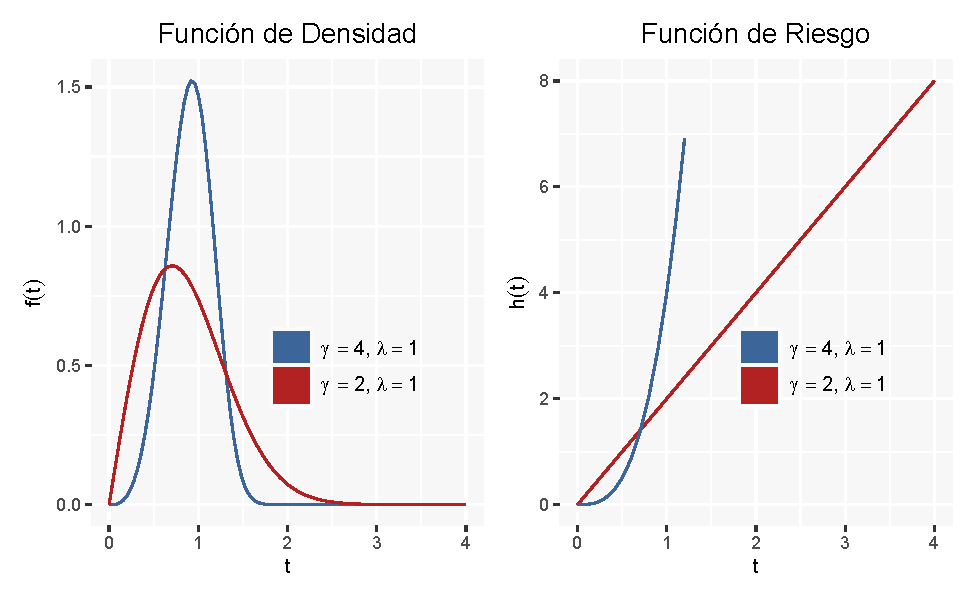
\includegraphics{_main_files/figure-latex/unnamed-chunk-16-1} \end{center}

Y para el modelo Weibull con \(\lambda=1\) y \(\gamma=0.5,1\) se tienen las siguientes gráficas:

\begin{center}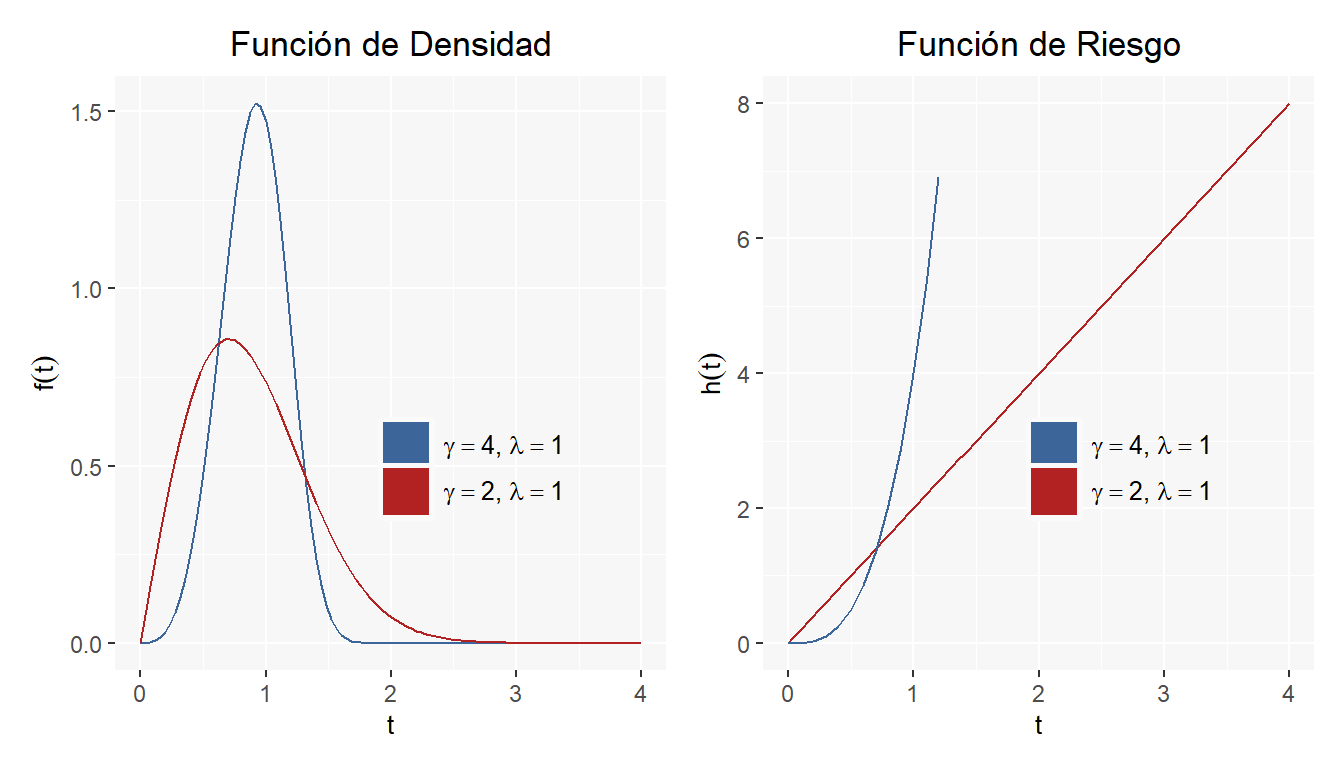
\includegraphics{_main_files/figure-latex/unnamed-chunk-17-1} \end{center}

Como bien hemos dicho, si suponemos una función de riesgo monótona creciente ó decreciente la distribución Weibull puede ser generada. Concretamente, si \(\gamma>1\) entonces \(h(t)\) es estrictamente creciente, si \(\gamma<1\) entonces \(h(t)\) es estrictamente decreciente. Cuando \(\gamma=1\) se tiene la distribución exponencial.

\textbf{R}

Para este caso el sufijo referente a esta distribución es \texttt{*weibull}, de tal manera que se tienen las siguientes funciones mencionando la interpretación de sus resultados:

\begin{itemize}
\tightlist
\item
  \texttt{rweibull(n,\ shape,\ scale\ =\ 1)}: Muestra pseudo aleatoria de tamaño \(n\).
\item
  \texttt{dweibull(x,\ shape,\ scale\ =\ 1,\ log\ =\ FALSE)}: Valores de \(f(x)\).
\item
  \texttt{pweibull(q,\ shape,\ scale\ =\ 1,\ lower.tail\ =\ TRUE,\ log.p\ =\ FALSE)}: Valores de \(F(x)\).
\item
  \texttt{qweibull(p,\ shape,\ scale\ =\ 1,\ lower.tail\ =\ TRUE,\ log.p\ =\ FALSE)}: Cuantil \(t_p\).
\end{itemize}

Así como en el caso de la exponencial y en todos los casos posteriores, se respeta el orden de los parámetros por lo que para aplicar los parámetros tal como se vieron en esta sección se puede utilizar esta función de la siguiente manera: \texttt{dweibull}(\(\gamma\), \(1/\lambda\)) o sin importar el orden indicando de manera explicita que \texttt{shape} = \(\gamma\) y \texttt{scale} = \(1/\lambda\). Esto último debido a que la función de densidad para este modelo en R esta considerada como \(f(x) = \frac{\gamma}{\lambda}(\frac{x}{\lambda})^{\gamma-1}e^{-(\frac{x}{\lambda})^\gamma}\).

\hypertarget{modelo-log-normal}{%
\section{Modelo Log-Normal}\label{modelo-log-normal}}

El modelo Log-Normal tiene estrecha relación con la distribución \emph{Normal}. De hecho, el tiempo de supervivencia \(T\) se dice que sigue una distribución Log-Normal, si \(Y=ln(T)\) se distribuye \(N(\mu,\sigma^2)\).

La distribución Log-Normal se ha utilizado como modelo en el tiempo de falla de aislantes eléctricos y en el tiempo de aparición de cáncer pulmonar. También se utiliza en poblaciones que son una mezcla de tiempos de vida cortos y largos. A pesar de esto, este modelo es criticado por ser decreciente para valores grandes de \(t\), lo cual parece inadecaudo en algunas situaciones.

\textbf{Función de Densidad}

Para este modelo, \(f(t)\) está dada por:

\[
f(t)=\frac{1}{\sqrt {2\pi}\sigma t}exp\left(-\frac{1}{2}\left(\frac{ln(t)-\mu}{\sigma}\right)^2\right)
\]

En este caso, \(\mu\) y \(\sigma\) pasan a ser los parámetros de escala y de forma de la distribución, los cuales hacen diferencia con los de la distribución normal, ya que en tal caso \(\mu\) sería un parámetro de localización y \(\sigma\) seguiría siendo el parámetro de escala. Para agregar un parámetro de localización a la distribución \(log-normal\) bastaría camiar \(x\) por \(x-\theta\) donde \(\theta\) sería tal parámetro.

\textbf{Función de Supervivencia}

\[
S(t)=\int_t^{\infty}f(u)du
\\=1-\int_0^{t}f(u)du
\\=1-\int_0^{t}\frac{1}{\sqrt {2\pi}\sigma u}exp\left(-\frac{1}{2}\left(\frac{ln(u)-\mu}{\sigma}\right)^2\right)du
\]

Tomando la notación de la función de distribución de una \emph{Normal estándar}, \(\Phi()\), se tiene:

\[
S(t)=1-\Phi\left(\frac{ln(t)-\mu}{\sigma}\right)
\]

\textbf{Función de Riesgo}

\[
h(t)=\frac{f(t)}{S(t)}
\\=\frac{\frac{1}{\sqrt {2\pi}\sigma t}exp\left(-\frac{1}{2}\left(\frac{ln(t)-\mu}{\sigma}\right)^2\right)}{1-\Phi\left(\frac{ln(t)-\mu}{\sigma}\right)}
\]

Si bien la expresión de \(h(t)\) parece ser complicada, su gráfica resulta ser más interesante. Ésta toma el valor de cero en \(t=0\), crece hasta un valor máximo y luego tiende a cero cuando \(t \rightarrow \infty\). Véase sección de gráficas.

\textbf{Parámetros}

Si \(T\sim LogNormal(\mu,\sigma^2)\) entonces:

\[
\mathbb{E}[T]=exp\left(\mu+\frac{\sigma^2}{2}\right)
\]

Y además

\[
Var[T]=exp(2\mu+2\sigma^2)-exp(2\mu+\sigma^2)
\]

La demostración de las igualdades de media y varianza se dejan al alumno.

\textbf{Gráficas}

A continuación algunos ejemplos de las gráficas de \(f(t)\) y \(h(t)\) para la distribución Log-Normal:

\begin{center}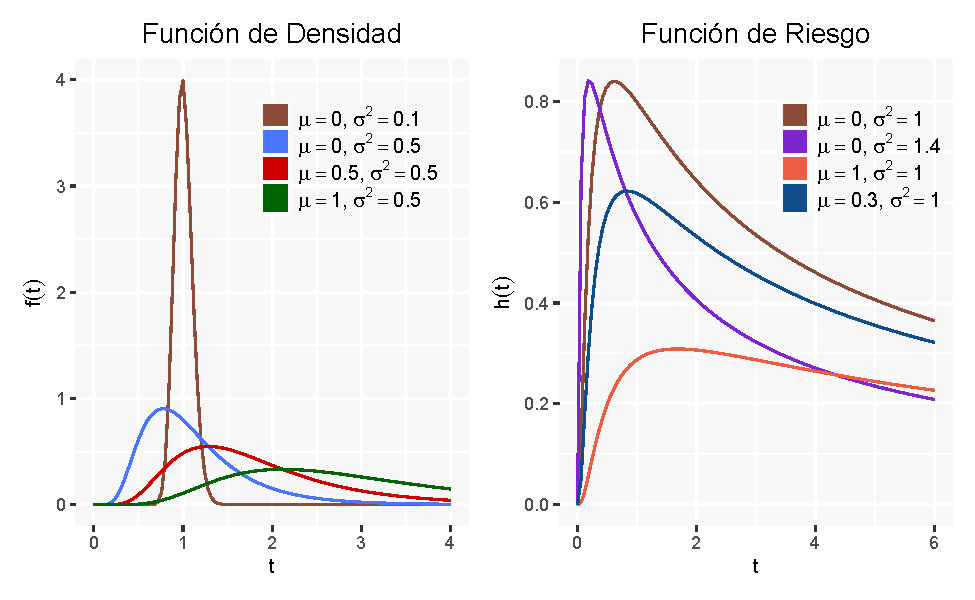
\includegraphics{_main_files/figure-latex/unnamed-chunk-18-1} \end{center}

\textbf{R}

Para esta distribución el sufijo respectivo será \texttt{*lnorm}, de tal manera que se tienen las siguientes funciones mencionando la interpretación de sus resultados:

\begin{itemize}
\tightlist
\item
  \texttt{rlnorm(n,\ meanlog\ =\ 0,\ sdlog\ =\ 1)}: Muestra pseudo aleatoria de tamaño \(n\).
\item
  \texttt{dlnorm(x,\ meanlog\ =\ 0,\ sdlog\ =\ 1,\ log\ =\ FALSE)}: Valores de \(f(x)\).
\item
  \texttt{plnorm(q,\ meanlog\ =\ 0,\ sdlog\ =\ 1,\ lower.tail\ =\ TRUE,\ log.p\ =\ FALSE)}: Valores de \(F(x)\).
\item
  \texttt{qlnorm(p,\ meanlog\ =\ 0,\ sdlog\ =\ 1,\ lower.tail\ =\ TRUE,\ log.p\ =\ FALSE)}: Cuantil \(t_p\).
\end{itemize}

En este caso, es evidente que \texttt{meanlog} correspondería al parámetro de escala \(\mu\) y \texttt{sdlog} al parámetro de forma \(\sigma\). Finalmente se menciona que estos parámetros no se deben confundir explícitamente con los de una distribución normal.

\hypertarget{ejemplo-6}{%
\subsubsection*{Ejemplo}\label{ejemplo-6}}


El tiempo de muerte en días después de un trasplante de médula sigue una distribución \(log-normal\) con \(\mu = 3.177, \sigma = 2.084\). Calcular lo siguiente

\begin{enumerate}
\def\labelenumi{\arabic{enumi}.}
\tightlist
\item
  La media y la mediano tiempo de muerte
\item
  La probabilidad de que un individuo sobreviva 200 días después de un trasplante.
\end{enumerate}

Soluciones

\begin{enumerate}
\def\labelenumi{\arabic{enumi}.}
\tightlist
\item
\end{enumerate}

\begin{itemize}
\tightlist
\item
  Mediana: \(t_{0.5} =e^{\mu}\) cuando \(T\sim log-normal \implies\) Mediana de tiempo de muerte: \(t_{0.5} = e^{3.177} = 23.97\).
\item
  Media: \(\mathbb{E}(T) = e^{\mu+\sigma^2/2}\) cuando \(T\sim log- normal \implies\) Media de tiempo de muerte: \(\mathbb{E}(T) = e^{3.177+\frac{(2.084)^2}{2}} = 210.29\) días.
\end{itemize}

Entonces si sobrevivieron 23.97, queda una gran cantidad de días donde, en promedio son 210.29.

\begin{enumerate}
\def\labelenumi{\arabic{enumi}.}
\setcounter{enumi}{1}
\tightlist
\item
  \(S(200) = 1-\Phi\left(\frac{\ln(200)-3.177}{2.084}\right) = 1-0.8438 = 0.15436\).
\end{enumerate}

\hypertarget{modelo-log-loguxedstico}{%
\section{Modelo Log-Logístico}\label{modelo-log-loguxedstico}}

El modelo Log-Logístico es derivado de la distribución \emph{Logística}. Se dice que \(T\) tiene distribución Log-Logística si \(Y=ln(T)\) sigue una distribución Logística con parámetros \(\mu\) y \(\sigma ^2\).

\textbf{Función de Densidad}

\[
f(t)=\frac{\alpha \lambda (\lambda t)^{\alpha-1}}{(1+(\lambda t)^\alpha)^2}
\]

con \(\alpha=\frac{1}{\sigma}\) y \(\lambda=exp(-\frac{\mu}{\sigma})>0\). \(\alpha\) es el parámetro de forma y \(\lambda\) es el parámetro de escala.

\textbf{Función de Supervivencia}

\[
S(t)=\frac{1}{1+(\lambda t)^\alpha}
\]

\textbf{Función de Riesgo}

\[
h(t)=\frac{f(t)}{S(t)}=\frac{\alpha \lambda (\lambda t)^{\alpha-1}}{1+(\lambda t)^\alpha}
\]

La función de riesgo es monótona decreciente para \(\alpha \leq 1\), y para \(\alpha> 1\) la función de riesgo crece hasta alcanzar un máximo en \(t=(\frac{\alpha-1}{\lambda})^{\frac{1}{\alpha}}\) y luego decrece a cero cuando \(t \rightarrow \infty\).

\textbf{Gráficas}

Algunos ejemplos de las gráficas de \(f(t)\) y \(h(t)\) para la distribución Log-Logística:

\begin{center}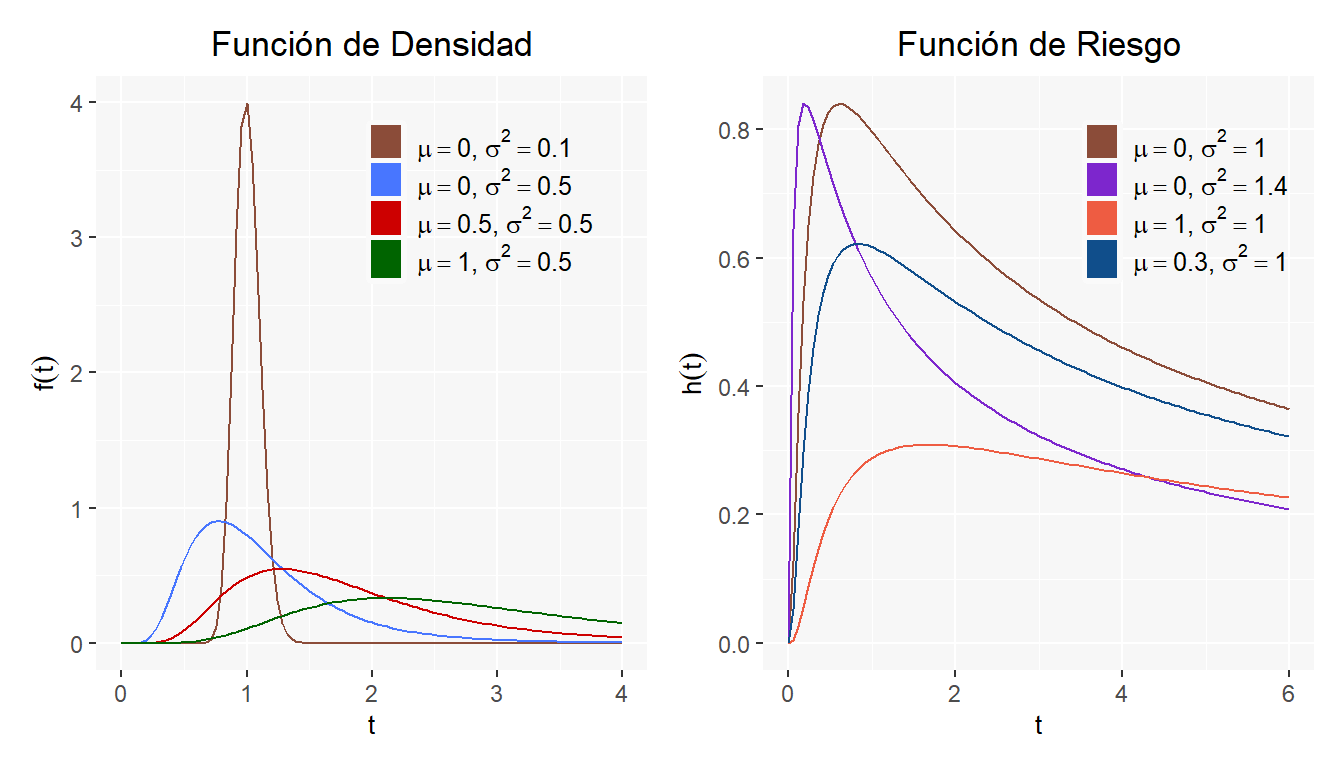
\includegraphics{_main_files/figure-latex/unnamed-chunk-19-1} \end{center}

\textbf{R}

Para esta distribución se recomienda descargar y utilizar el paquete \texttt{actuar}, en la cual vienen un conjunto de funciones similares a las anteriores, de hecho el sufijo respectivo será \texttt{*llogis} y, de manera análoga a las anteriores funciones, se tiene lo siguiente:

\begin{itemize}
\tightlist
\item
  \texttt{rllogis(n,\ shape,\ rate\ =\ 1,\ scale\ =\ 1/rate)}: Muestra pseudo aleatoria de tamaño \(n\).
\item
  \texttt{dllogis(x,\ shape,\ rate\ =\ 1,\ scale\ =\ 1/rate,\ log\ =\ FALSE)}: Valores de \(f(x)\).
\item
  \texttt{pllogis(q,\ shape,\ rate\ =\ 1,\ scale\ =\ 1/rate,\ lower.tail\ =\ TRUE,\ log.p\ =\ FALSE)}: Valores de \(F(x)\).
\item
  \texttt{qllogis(p,\ shape,\ rate\ =\ 1,\ scale\ =\ 1/rate,\ lower.tail\ =\ TRUE,\ log.p\ =\ FALSE)}: Cuantil \(t_p\).
\end{itemize}

En este caso, como en la exponencial y la weibull, \texttt{rate} correspondería al parámetro \(\lambda\) y \texttt{shape} al parámetro de forma \(\alpha\).

\hypertarget{modelo-gamma}{%
\section{Modelo Gamma}\label{modelo-gamma}}

La distribución Gamma, que incluye a las distribuciones \emph{exponencial} y \emph{ji-cuadrada}, ha sido utilizada como un modelo para problemas de confiabilidad industrial, hepatogramas en adultos normales y en pacientes con cirrosis, en supervivencia de plaquetas, entre otros. Este modelo tiene dos parámetros: \(\beta\) es el parámetro de forma y \(\lambda\) es el parámetro que modifica de escala; estrictamente hablando \(\lambda\) es la tasa: \(\lambda =\frac{1}{s}\) donde \(s\) sería el verdadero parámetro de escala.

\textbf{Función de Densidad}

\(f(t)\) está dada por:

\[
f(t)=\frac{\lambda^\beta}{\Gamma(\beta)}t^{\beta-1}exp(-\lambda t); \ \ \  \lambda,\beta>0
\]

\textbf{Función de Supervivencia}

\[
S(t)=1-Ig(\lambda t, \beta)
\]

donde\footnote{Esta función se llama \emph{función gamma incompleta} y en algunas fuentes se puede encontrar esta en particular como \emph{\textbf{lower incomplete gamma function}}. Cuando se tiene \(\int_x^{\infty}u^{\beta-1}e^{-u}du = \Gamma(x, \beta)\) se le conoce como \emph{\textbf{upper incomplete gamma function}}, la cual es una \href{https://mathworld.wolfram.com/IncompleteGammaFunction.html}{generalización} de la función gamma: \(\Gamma(x, 0) = \Gamma(x)\). Originalmente esta función no tiene el cociente que se esta utilizando en este caso, esto es un efecto de normalizar la función como se puede ver en el siguiente \href{https://dlmf.nist.gov/8.2}{enlace}. Algunas veces esta función es conocida directamente como función gamma incompleta como en \citep{klein2006survival}}:

\[
Ig(t,\beta)=\frac{1}{\Gamma(\beta)}\int_0^{t}u^{\beta-1}e^{-u}du
\]
Al igual que un modelo \(Weibull(\lambda, alpha = 1)\), la distribución exponencial es un caso particular del modelo \(Gamma(\lambda,\beta = 1)\). Cuando \(\beta \rightarrow\infty\), modelo gamma se aproxima a una distribución normal.

\textbf{Función de Riesgo}

\[
h(t)=\frac{f(t)}{S(t)}=\frac{\frac{\lambda^\beta}{\Gamma(\beta)}t^{\beta-1}exp(-\lambda t)}{1-Ig(\lambda t, \beta)}
\]

Esta función de riesgo tiene distintos comportamientos:

\begin{itemize}
\tightlist
\item
  Es \textbf{monótona creciente} para \(\beta>1\). En este caso sucede que \(h(0)=0\) y \(\underset{t\rightarrow\infty}{h(t)} \rightarrow \lambda\). Además, la moda de la distribución es \(t = \frac{\beta-1}{\lambda}\)
\item
  Es \textbf{monótona decreciente} con \(\beta <1\). En tal caso \(h(0) = \infty\) y \(\underset{t\rightarrow\infty}{h(t)} \rightarrow \lambda\).
\end{itemize}

\textbf{Parámetros}

Si \(T\sim Gamma(\beta,\lambda)\) entonces:

\[
\begin{array}{ccc}
\mathbb{E}[T]=\frac{\beta}{\lambda} & \mbox{y} &
Var[T]=\frac{\beta}{\lambda^2}
\end{array}
\]

Las demostraciones de las igualdades de la esperanza y varianza se quedan de ejercicio al alumno.

\textbf{Gráficas}

Se muestran ejemplos de las gráficas de \(f(t)\) y \(h(t)\) para el modelo Gamma:

\begin{center}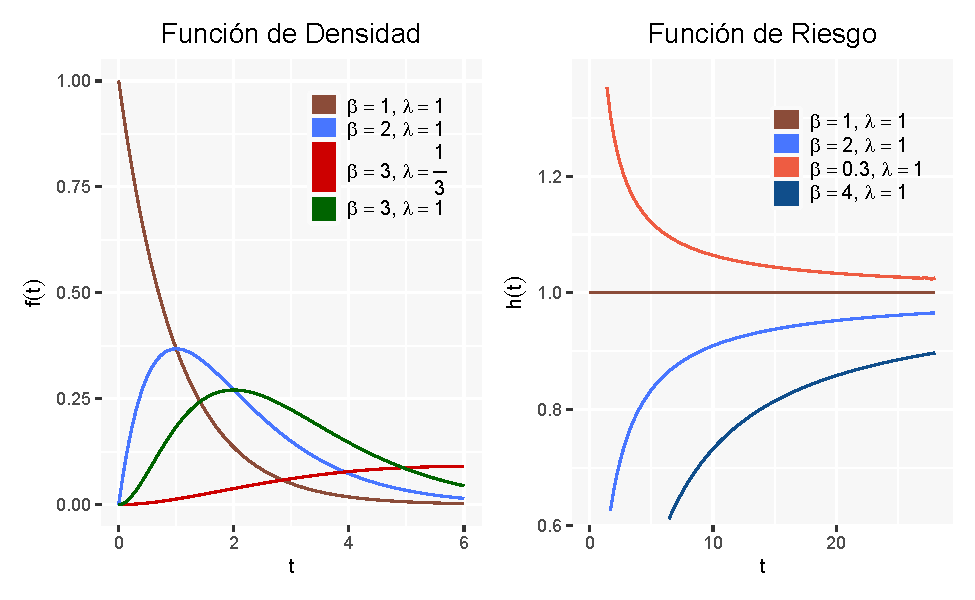
\includegraphics{_main_files/figure-latex/unnamed-chunk-20-1} \end{center}

\textbf{R}

Para esta distribución el sufijo respectivo será \texttt{*gamma}, de tal manera que se tienen las siguientes funciones mencionando la interpretación de sus resultados:

\begin{itemize}
\tightlist
\item
  \texttt{rgamma(n,\ shape,\ rate\ =\ 1,\ scale\ =\ 1/rate)}: Muestra pseudo aleatoria de tamaño \(n\).
\item
  \texttt{dgamma(x,\ shape,\ rate\ =\ 1,\ scale\ =\ 1/rate,\ log\ =\ FALSE)}: Valores de \(f(x)\).
\item
  \texttt{pgamma(q,\ shape,\ rate\ =\ 1,\ scale\ =\ 1/rate,\ lower.tail\ =\ TRUE,\ log.p\ =\ FALSE)}: Valores de \(F(x)\).
\item
  \texttt{qgamma(p,\ shape,\ rate\ =\ 1,\ scale\ =\ 1/rate,\ lower.tail\ =\ TRUE,\ log.p\ =\ FALSE)}: Cuantil \(t_p\).
\end{itemize}

Como en el caso de la exponencial, se recomienda tener precaución ya que el parámetro \texttt{rate} es el que corresponde al parámetro \(\lambda\) en este trabajo.

\hypertarget{modelo-gamma-generalizada}{%
\section{Modelo Gamma Generalizada}\label{modelo-gamma-generalizada}}

Finalmente, se presenta el modelo Gamma Generalizada con dos parámetros de forma y un parámetro de que modifica la escala \(\alpha\), \(\beta\) y \(\lambda\) respectivamente.

\textbf{Función de Densidad}

\(f(t)\) está dada por:

\[
f(t)=\frac{\alpha\lambda^{\beta\alpha}}{\Gamma(\beta)}t^{\alpha\beta-1}\exp(-\lambda t)^\alpha; \ \ \  \lambda,\alpha, \beta>0
\]

\textbf{Función de Supervivencia}

\[
S(t)=1-Ig((\lambda t)^\alpha, \beta)
\]

Esta distribución se reduce a las siguientes

\begin{itemize}
\tightlist
\item
  \(Exponencial\) cuando \(\beta = \alpha = 1\).
\item
  \(Weibull\) cuando \(\beta = 1\).
\item
  \(Gamma\) cuando \(\alpha = 1\).
\item
  Tiende a la log-normal cuando \(\beta\rightarrow\infty\).
\end{itemize}

\textbf{R}

Para esta distribución se recomienda descargar y utilizar el paquete \texttt{ggamma}, en la cual vienen un conjunto de funciones similares a las anteriores. Aquí el respectivo sufijo será \texttt{*ggamma} y, de manera análoga a las anteriores funciones, se tiene lo siguiente:

\begin{itemize}
\tightlist
\item
  \texttt{rggamma(n,\ a,\ b,\ k)}: Muestra pseudo aleatoria de tamaño \(n\).
\item
  \texttt{dggamma(x,\ a,\ b,\ k,\ log\ =\ F)}: Valores de \(f(x)\).
\item
  \texttt{pggamma(p,\ a,\ b,\ k,\ lower.tail\ =\ TRUE,\ log.p\ =\ FALSE)}: Valores de \(F(x)\).
\item
  \texttt{qggamma(p,\ shape,\ rate\ =\ 1,\ scale\ =\ 1/rate,\ lower.tail\ =\ TRUE,\ log.p\ =\ FALSE)}: Cuantil \(t_p\).
\end{itemize}

Para este caso, se tiene una parametrización de uso común en distintas fuentes. \texttt{a} = \(\frac{1}{\lambda}\), \texttt{b} = \(\alpha\) y \texttt{k} = \(\beta\).

\hypertarget{ejemplo-7}{%
\subsubsection*{Ejemplo}\label{ejemplo-7}}


El tiempo de vida en meses de cierta especie de ratón sigue una distribución \(gamma(\beta = 3, \lambda = 0.2)\).

\begin{enumerate}
\def\labelenumi{\arabic{enumi}.}
\tightlist
\item
  Calcular la probabilidad de que un ratón sobreviva más de 18 meses.
\item
  ¿Cuál es la probabilidad de que un ratón muera en el primer año de vida?
\item
  ¿Cuál es la esperanza de vida media de esta especia?
\end{enumerate}

Soluciones

\begin{enumerate}
\def\labelenumi{\arabic{enumi}.}
\tightlist
\item
  \(S(18) = 1-F(18) = 1-\) 0.6972532 = 0.3027468
\item
  \(F(12) =\) 0.4302913
\item
  \(\mathbb{E}(T) = \frac{\beta}{\lambda} = \frac{3}{0.2} = 15\) meses.
\end{enumerate}

Cabe señalar que hasta este punto \textbf{no hemos introducido datos censurados a los modelos}.

\hypertarget{la-funciuxf3n-de-verosimilitud-con-censura-y-truncamiento}{%
\chapter{La Función de Verosimilitud con Censura y Truncamiento}\label{la-funciuxf3n-de-verosimilitud-con-censura-y-truncamiento}}

Cuando se conoce la distribución de \(T\), hacer estimaciones (usualmente por el método de máxima verosimilitud) sobre parámetros poblacionales resulta de suma importancia, pues a partir de ellos no sólo podemos conocer \emph{estimadores} de la media, varianza o cuantiles; sino que también podemos conocer \(\hat S(t)\), \(\hat h(t)\), etc. En la sección anterior revisamos los modelos paramétricos más usados en análisis de supervivencia, sin embargo, no contemplamos datos censurados o truncados en dichos modelos. En este apartado veremos la función de verosimilitud considerando censura y truncamiento, y con base en esta función haremos estimaciones para algunas distribuciones.

\hypertarget{caso-general}{%
\section{Caso General}\label{caso-general}}

De acuerdo al tipo de observación, se tienen las siguientes contribuciones a la función de verosimilitud:

\[
\begin{array}{ll}
\mbox{Exactas } T_{i} & f(t_{i})\\
\mbox{Censurada por la derecha } T_{i}>C_{i} & \mathbb{P}(T_{i}>C_{i})=S(C_{i})\\
\mbox{Censurada por la izquierda } T_{i}<C_{i} & \mathbb{P}(T_{i}<C_{i})=1-S(C_{i})\\
\mbox{Censurada por la intervalo } L_{i}<T_{i}\leq R_{i} & \mathbb{P}(L_{i}<T_{i}\leq R_{i})=S(L_{i})-S(R_{i})\\
\mbox{Truncado por la izquierda } T_{i}|T_{i}>u_{i} & \mathbb{P}(T_{i}|T_{i}>u_{i})=\frac{f(t_{i})}{S(u_{i})}\\
\mbox{Truncado por la derecha } T_{i}|T_{i} \leq v_{i} & \mathbb{P}(T_{i}|T_{i} \leq v_{i})=\frac{f(t_{i})}{1-S(v_{i})}\\
\end{array}
\]

Entonces la función de verosimilitud es:

\[
\mathbf{\mathscr{L}} = \prod_{i\in D}f(t_{i})\prod_{i\in R}S(C_{i})\prod_{i\in L}(1-S(C_{i}))\prod_{i\in I}[S(L_{i})-S(R_{i})]
\]
donde

\begin{itemize}
\tightlist
\item
  D: Conjunto de tiempos de fallo.
\item
  R: Conjunto de observaciones censuradas por la derecha.
\item
  L: Conjunto de observaciones censuradas por la izquierda.
\item
  I: Conjunto de observaciones censuradas por intervalo.
\end{itemize}

Cuando hay datos truncados, se sustituye \(f(t_{i})\) por \(\frac{f(t_{i})}{S(u_{i})}\) y \(S(C_{i})\) por \(\frac{S(C_{i})}{S(_{u_{i}})}\).

\hypertarget{censura-por-la-derecha-tipo-i-1}{%
\section{Censura por la Derecha Tipo I}\label{censura-por-la-derecha-tipo-i-1}}

Suponga que se tiene una muestra aleatoria de \(n\) individuos con tiempos de vida \(T_1,T_2,..., T_n\)(v.a.i.i.d) y que está asociado a cada individuo un tiempo fijo de censura \(C_i>0\). Se observa a \(T_i\) solamente si \(T_i\leq C_i\), por lo que los datos son parejas: \((t_i,\delta_i)\), \(i=1,2,...,n\) donde \(t_i=min(T_i,C_i)\) y:

\[
\delta_{i} = \left\{
\begin{array}{ll}
0 & \mbox{si }  t_{i} \ = \ C_i\\
1 & \mbox{si }  t_{i} \ =\ T_i
\end{array}
\right.
\]

Entonces la función de verosimilitud para datos con este tipo de censura es de la forma:

\[ 
\mathscr{L} = \prod^{n}_{i=1}f(t_{i})^{\delta_{i}}S(t_{i})^{1-\delta_{i}} 
\]

donde \(\sum_{i=1}^{n}\delta_i\) representa el total de los tiempos de vida observados.

Considerando que \(f(t) = h(t) S(t)\), entonces:

\[
\begin{split}
\mathscr{L} & =\prod_{i = 1}^{n}h(t_{i})^{\delta_{i}}S(t_{i})^{\delta_{i}}S(t_{i})^{1-\delta_{i}}\\
 & =\prod_{i = 1}^{n}h(t_{i})^{\delta_{i}}S(t_{i})\\
 & =\prod_{i = 1}^{n}h(t_{i})^{\delta_{i}}exp\{-H(t_{i})\}
\end{split}
\]

\hypertarget{censura-por-la-derecha-tipo-ii-1}{%
\section{Censura por la Derecha Tipo II}\label{censura-por-la-derecha-tipo-ii-1}}

Supongamos que se observan los \(r\) tiempos de falla \(T_{(1)}< T_{(2)}< ...<T_{(r)}\) más pequeños, dejando a \(n-r\) tiempos censurados por la derecha, de una muestra de tamaño \(n\). De modo que, los datos serán los \(r\) tiempos de fallo más pequeños de \(T_{1}, T_{2},...,T_{n}\).

\(T\) tiene f.d.p \(f(t)\) y función de supervivencia \(S(t)\). Entonces la f.d.p. conjunta de \(T_{(1)}, T_{(2)}, ...,T_{(r)}\) es:

\[
\mathscr{L} = \frac{n!}{(n-r)!}\left\{\prod_{i=1}^{r}f(t_{i})\right\}\left[S\left(t_{(r)}\right)\right]^{n-r}
\]

donde \(\prod_{i=1}^{r}f(t_{i})\) es la parte correspondiente a las \(r\) fallas observadas y \([S(t_{(r)})]^{n-r}\) constituye la aportación de las observaciones censuradas después de la \(r-esima\) falla observada.

Observemos que si quitamos el término constante \(\frac{n!}{(n-r)!}\) y definiendo a la función indicadora:

\[
\delta_{i} = \left\{
\begin{array}{ll}
0 & \mbox{si  } T_{i} \ > \ T_{(r)}\\
1 & \mbox{si }  T_{i}  \leq\ T_{(r)}
\end{array}
\right.
\]

Entonces la función de verosimilitud para este tipo de censura se puede reesctibir:

\[ 
\mathscr{L} \propto \prod^{n}_{i=1}f(t_{i})^{\delta_{i}}S(t_{i})^{1-\delta_{i}} 
\]

que es la función de verosimilitud con datos censurados por la derecha tipo 1 revisada en la sección anterior.

\hypertarget{censura-aleatoria}{%
\section{Censura Aleatoria}\label{censura-aleatoria}}

Supongamos que para cada individuo se tienen \(T_i\) y \(C_i\) variables aleatorias independientes, con funciones de densidad \(f_{T}(t)\) y \(f_{C}(t)\), y con funciones de superviviencia \(S_{T}(t)\) y \(S_{C}(t)\) respectivamente. Sean \((T_i,C_i)\), \(i=1,2,...,n\) parejas de observaciones independientes, la variable que observamos es \(t_i=min(T_i,C_i)\) y se define:

\[
\delta_{i} = \left\{
\begin{array}{ll}
0 & \mbox{si  } T_{i} \ > \ C_i\\
1 & \mbox{si }  T_{i}  \leq\ C_i
\end{array}
\right.
\]

por lo que, las observaciones son las parejas \((t_i,\delta_i)\) con \(i=1,2,...,n\).

La función de verosimilitud es entonces:

\[ 
\mathscr{L} = \prod^{n}_{i=1}[S_C(t_{i})]^{1-\delta_{i}}[f_C(t_i)]^{\delta_i}[f_T(t_i)]^{\delta_i}[S_T(t_{i})]^{1-\delta_{i}} 
\]

Similar al caso se censura por la derecha tipo 2, se puede demostrar que la expresión anterior es proporcional a \(\prod^{n}_{i=1}f_T(t_{i})^{\delta_{i}}S_T(t_{i})^{1-\delta_{i}}\).

\hypertarget{truncamiento-por-la-izquierda}{%
\section{Truncamiento por la Izquierda}\label{truncamiento-por-la-izquierda}}

Consideremos los tiempos de fallo truncados por la izquierda, es decir, \(T_{i}\) tal que \(T_{i}\geq u_{i}\) para ser observado (\(u_{i}\) es el valor de truncamiento).

En este caso, las observaciones serán \((u_{i}, t_{i},\delta_{i})\) con \(t_{i}\geq u_{i}\) tiempo de fallo y \(\delta_{i}\) indicador de censura por la derecha. Por lo que:

\[
\mathbf{\mathscr{L}} = \prod_{i=1}^{n}\left\{\frac{f(t_{i})}{S(u_{i})}\right\}^{\delta_{i}}\left\{\frac{S(t_{i})}{S(u_{i})}\right\}^{1-\delta_{i}}=\prod_{i=1}^{n}\left\{h(t_{i})\right\}^{\delta_{i}}\left\{\frac{S(t_{i})}{S(u_{i})}\right\}
\]

Obsérvese que el hecho de dividir la función de verosimilitud entre \(S(u_{i})\) se limita a que los datos sean truncados por la izquierda\footnote{De primera vista, pareciera que la segunda igualdad de la expresión anterior es incorrecta y que debería ser \(\prod_{i=1}^{n}\left\{h(t_{i})\right\}^{\delta_{i}}\left\{\frac{S(t_{i})}{S(u_{i})}\right\}^{1-\delta_i}\) lo cual no es correcto. Se recomienda desarrollar la primera igualdad y relacionar lo necesario para obtener \(h(t_i)\).}.

\hypertarget{truncamiento-por-la-derecha}{%
\section{Truncamiento por la Derecha}\label{truncamiento-por-la-derecha}}

Consideremos tiempos de fallo \(T_{i}\) tal que \(T_{i} \leq v_{i}\) para que sea observado. Entonces las observaciones serán \((t_{i}, v_{i})\) para todo \(i = 1,...,n\).

Por lo que:

\[
\mathbf{\mathscr{L}} = \prod_{i=1}^{n}\left\{\frac{f(t_{i})}{1-S(v_{i})}\right\} =\prod_{i=1}^{n} \mathbb{P}(T_{i}|T_{i}<v_{i})
\]

\hypertarget{estimaciones-para-algunos-modelos}{%
\section{Estimaciones para Algunos Modelos}\label{estimaciones-para-algunos-modelos}}

\hypertarget{modelo-exponencial-1}{%
\subsection*{Modelo Exponencial}\label{modelo-exponencial-1}}


Sean los tiempos de fallo \(T_{i}\) independientes y provenientes de una distribución exponencial:

\begin{itemize}
\tightlist
\item
  \(f(t) = \lambda e^{-\lambda t}\)
\item
  \(S(t) = e^{-\lambda t}\)
\item
  \(h(t) = \lambda\)
\item
  \(H(t) = \lambda t\)
\end{itemize}

Entonces, la función de verosimilitud con censura tipo I es:

\[
\mathscr{L} = \prod_{i}^{n}\lambda^{\delta_{i}}e^{-\lambda t_{i}}= \lambda^{\sum_{i= 1}^{n}\delta_{i}}e^{-\lambda \sum_{i = 1}^{n}t_{i}}
\]

Sea \(r=\sum_{i = 1}^{n}\delta_{i}\) el número de observaciones exactas (no censuradas). Entonces:

\[
 \mathscr{L} = \lambda^{r}e^{-\lambda\sum_{i= 1}^{n}t_{i}}
\]

Si queremos un estimador para \(\lambda\), hacemos:

\[
\frac{\partial ln(\mathscr{L})}{\partial \lambda} = \frac{\partial[r ln(\lambda)-\lambda\sum_{i = 1}^{n}t_{i}]}{\partial\lambda} = \frac{r}{\lambda}-\sum_{i  =1}^{n}t_i = 0
\]

\[
\Longrightarrow \hat{\lambda} = \frac{r}{\sum_{i= 1}^{n}t_{i}}
\]

Observe que si \emph{no hay datos censurados} entonces \(\sum_{i = 1}^{n}\delta_{i}=n\), por lo que \(\hat{\lambda}=\frac{1}{\bar t}\), y este es el estimador que conocemos desde el curso de inferencia.

\hypertarget{ejemplo-8}{%
\subsubsection*{Ejemplo}\label{ejemplo-8}}


El siguiente ejercicio fue basado en el ejercicio 3.6 del libro \citep{klein2006survival}. Los siguientes datos consisten en los tiempos de recaída y los tiempos de muerte después de la recaída de 10 pacientes con trasplante de médula ósea. Suponga que el tiempo hasta la recaída tiene una distribución exponencial con la tasa de riesgo \(\lambda\).

\begin{table}
\centering
\begin{tabular}{cc}
\toprule
Paciente & Tiempo de recaida en meses\\
\midrule
1 & 5\\
2 & 8\\
3 & 12\\
4 & 24\\
5 & 32\\
\addlinespace
6 & 17\\
7 & 16+\\
8 & 17+\\
9 & 19+\\
10 & 30+\\
\bottomrule
\multicolumn{2}{l}{\rule{0pt}{1em}Los datos censurados están representados con un '+'}\\
\end{tabular}
\end{table}

\begin{itemize}
\item
  \begin{enumerate}
  \def\labelenumi{\alph{enumi})}
  \tightlist
  \item
    Calcule la tasa de recaída.
  \end{enumerate}
\item
  \begin{enumerate}
  \def\labelenumi{\alph{enumi})}
  \setcounter{enumi}{1}
  \tightlist
  \item
    Calcule la probabilidad de no recaer en 16 meses.
  \end{enumerate}
\end{itemize}

Sabemos que los estimadores máximo-verosímiles cumplen la propiedad de invarianza, de modo que:

\begin{enumerate}
\def\labelenumi{\alph{enumi})}
\item
  \(\hat{\lambda} = \frac{r}{\sum_{i= 1}^{n}t_{i}} = \frac{6}{\sum_{i= 1}^{10}t_{i}} = \frac{6}{180} = 3.3333333\%\)
\item
  \(\hat S(16) = e^{-\hat\lambda t} = e^{-0.033(16)} = 0.5866463\)
\end{enumerate}

\hypertarget{modelo-weibull-1}{%
\subsection*{Modelo Weibull}\label{modelo-weibull-1}}


Supongamos que se tienen los tiempos de fallo \(T_{i}\) con censura, provenientes de una distribución Weibull:

\begin{itemize}
\tightlist
\item
  \(f(t) = \lambda \gamma(\lambda t)^{\gamma-1}e^{-(\lambda t)^\gamma}\)
\item
  \(S(t) = e^{-(\lambda t)^\gamma}\)
\item
  \(h(t) = \lambda \gamma(\lambda t)^{\gamma-1}\)
\end{itemize}

Entonces, su respectiva función de verosimilitud es de la forma:

\[
\mathscr{L} = \prod_{i}^{n}\left[\lambda \gamma(\lambda t_i)^{\gamma-1}e^{-(\lambda t_i)^\gamma}\right]^{\delta_i}\left[e^{-(\lambda t_i)^\gamma}\right]^{1-\delta_i} = \prod_{i}^{n}\left[\lambda \gamma(\lambda t_i)^{\gamma-1}\right]^{\delta_i}\left[e^{-(\lambda t_i)^\gamma}\right]
\]

Por lo que:

\[
\ln(\mathscr{L}) = \sum_{i=1}^{n}\delta_i\ln(\lambda \gamma(\lambda t_i)^{\gamma -1})-(\lambda t_i)^\gamma
\]

Si suponemos que \(r=\sum_{i = 1}^{n}\delta_{i}\) y desarrollamos la expresión anterior, obtenemos:

\[
\ln(\mathscr{L}) =r\ln(\lambda \gamma)+(\gamma -1)r\ln (\lambda)+(\gamma -1)\sum_{i=1}^{n}\delta_i\ln(t_i)-\lambda^{\gamma}\sum_{i=1}^{n}t_i^{\gamma}
\]

Los estimadores máximo-verosímiles de \(\lambda\) y \(\gamma\) se obtienen derivando \(\ln(\mathscr{L})\) con respecto a \(\lambda\) y \(\gamma\), igualando a cero y evaluando en \(\hat \lambda\) y \(\hat \gamma\):

\[
\frac{\partial \ln(\mathscr{L})}{\partial \lambda}=r\frac{\gamma}{\lambda \gamma}+\frac{(\gamma-1)r}{\lambda}-\gamma \lambda^{\gamma -1}\sum_{i=1}^{n}t_i^{\gamma}=0
\]

\[
\frac{\partial \ln(\mathscr{L})}{\partial \gamma}=r\frac{\lambda}{\lambda \gamma}+r\ln(\lambda)+\sum_{i=1}^{n}\delta_i\ln(t_i)-\left[\lambda^{\gamma}\ln(\lambda)\sum_{i=1}^{n}t_i^{\gamma}+\lambda^\gamma \sum_{i=1}^{n}t_i^{\gamma}\ln(t_i)\right]=0
\]

Simplificando ambas ecuaciones tenemos:

\[
r\gamma-\gamma \lambda^\gamma\sum_{i=1}^{n}t_i^\gamma=0
\]

\[
\frac{r}{\gamma}+r\ln(\lambda)+\sum_{i=1}^{n}\delta_i\ln(t_i)-\lambda^\gamma\left[\ln(\lambda)\sum_{i=1}^{n}t_i^{\gamma}-\sum_{i=1}^{n}t_i^{\gamma}\ln(t_i)\right]=0
\]

Despejamos a \(\lambda\) de la primera ecuación:

\[
\hat\lambda=\left(\frac{r}{\sum_{i=1}^{n}t_i^{\hat\gamma}}\right)^{\frac{1}{\hat\gamma}}
\]

Y sustituyendo en la segunda ecuación:

\[
\begin{array}{cc}
\frac{r}{\hat\gamma}+r\ln\left(\left(\frac{r}{\sum_{i=1}^{n}t_i^{\hat\gamma}}\right)^{\frac{1}{\hat \gamma}}\right)+\sum_{i=1}^{n}\delta_i\ln(t_i)&\\
-\left(\frac{r}{\sum_{i=1}^{n}t_i^{\hat \gamma}}\right)\left[\ln\left(\left(\frac{r}{\sum_{i=1}^{n}t_i^{\hat \gamma}}\right)^{\frac{1}{\hat \gamma}}\right)\sum_{i=1}^{n}t_i^{\hat \gamma}-\sum_{i=1}^{n}t_i^{\hat \gamma}\ln(t_i)\right]&=0
\end{array}
\]

La expresión anterior es una ecuación \emph{no lineal} de \(\hat \gamma\), cuya solución es únicamente mediante un método numérico. Una vez que se ha obtenido el valor \(\hat \gamma\), éste se sustituye en \(\left(\frac{r}{\sum_{i=1}^{n}t_i^{\hat \gamma}}\right)^{\frac{1}{\hat \gamma}}\) para así obtener, finalmente, el valor de \(\hat \lambda\).

Ecuaciones \emph{no lineales}, como hemos visto en el modelo \emph{Weibull}, aparecen en la estimación de parámetros de las distribuciones \emph{Log-Normal}, \emph{Log-Logística} y \emph{Gamma}; resulta que, al considerar datos con censura y truncamiento, las estimaciones se complican en los modelos paramétricos. No obstante, tenemos ayuda de las computadoras y software que nos permitirán realizar estimaciones adecuadas.

\hypertarget{part-estudio-no-paramuxe9trico}{%
\part{Estudio no paramétrico}\label{part-estudio-no-paramuxe9trico}}

\hypertarget{modelos-no-paramuxe9tricos-para-la-funciuxf3n-de-supervivencia}{%
\chapter{Modelos No Paramétricos para la Función de Supervivencia}\label{modelos-no-paramuxe9tricos-para-la-funciuxf3n-de-supervivencia}}

Los métodos estadísticos más utilizados en el análisis de supervivencia son los \emph{No Paramétricos}. Debido a que sólo cuando se conoce la distribución que siguen los tiempos de falla, las estimaciones con métodos paramétricos será adecuada. La eficiencia de los métodos no paramétricos radica en que los datos no sigan una distribución teórica.

Puesto que nuestro interés es estimar \(S(t)\), en los métodos no paramétricos las curvas de supervivencia, por lo general, se producen usando uno de dos métodos: el \textbf{análisis actuarial} o el \textbf{método límite-producto de Kaplan-Meier}.

Es importante mencionar que, cuando \textbf{no} hay datos censurados podemos estimar \(S(t)\) de manera sencilla mediante la función empírica:

\[
\hat S(t) = \hat{\mathbb{P}}(T>t) = \frac{ \# t_{i}>t}{n}
\]

donde la muestra aleatoria es: \(t_{(1)}\leq t_{(2)}\leq...\leq t_{(n)}\).

En este caso, la función será escalonada con decrementos \(\frac{1}{n}\) si todas las observaciones son distintas, o con decrementos \(\frac{d}{n}\) si hay \(d\) tiempos de falla iguales a \(t\).

Los métodos que se presentan a continuación incluyen la percepción del censuramiento en los datos; quizá el alumno está familiarizado con alguno de ellos, pues se estudian en cursos previos.

\hypertarget{muxe9todo-actuarial-tabla-de-vida}{%
\section{Método Actuarial (Tabla de Vida)}\label{muxe9todo-actuarial-tabla-de-vida}}

El análisis actuarial divide el tiempo en intervalos y calcula la supervivencia en cada intervalo. La longitud del intervalo depende de la frecuencia con que ocurre el suceso de interés.

Se asume que:

\begin{itemize}
\tightlist
\item
  Todos los abandonos durante un intervalo dado ocurren aleatoriamente durante dicho intervalo.
\item
  Las personas que se retiran del estudio tienen un destino parecido a las que se quedan.
\item
  El periodo de tiempo durante el cual una persona entra en el estudio no tiene efecto en la respuesta.
\end{itemize}

Dividimos el eje del tiempo en \(k+1\) intervalos \(l_{j}=(a_{j-1},a_{j}]\). Entonces para cada elemento de una muestra aleatoria de tamaño \(n\), se observa un tiempo de fallo \(T\) o un valor censurado por la derecha \(C\).

Definimos:

\begin{itemize}
\tightlist
\item
  \(n_{j}\): número de individuos en riesgo (vivos o no censurados) al tiempo \(a_{j-1}\).
\item
  \(d_{j}\): número de fallas en el intervalo \(l_{j}\).
\item
  \(c_{j}\): número de individuos que se censuran en el intervalo \(l_{j}\).
\end{itemize}

El número de individuos sin falla al inicio de \(l_{j}\) es \(n_{j}\).

Suponga que la función de supervivencia para los tiempos de falla es \(S(t) = \mathbb{P}(T>t)\). Entonces:

\[
S(a_{j}) = \mathbb{P}(T>a_{j}) = \mathbb{P}(T>a_{0})\mathbb{P}(T>a_{1}|T>a_{0})...\mathbb{P}(T>a_{j}|T>a_{j-1})
\]

Sea:

\begin{itemize}
\tightlist
\item
  \(S_{j} = S(a_{j})\)
\item
  \(p_{j} = \mathbb{P}(T>a_{j}|T>a_{j-1}) =\frac{S_{j}}{S_{j-1}}\) (Sobrevivencia hasta \(a_{j}\) después de haber sobrevivido hasta \(a_{j-1}\))
\item
  \(q_{j} = 1-p_{j} = \mathbb{P}(T\leq a_{j}|T>a_{j-1}) = \frac{S_{j-1}-S_{j}}{S_{j-1}}\) (No sobrevivir hasta \(a_{j}\) después de haber sobrevivido hasta \(a_{j-1}\))
\end{itemize}

Donde \(S_{0} = 1\), \(S_{k+1} = 0\), \(q_{k+1} = 1\). Por lo tanto:

\[
S_{j} = p_{1}p_{2}...p_{j}
\]

El objetivo es estimar \(S_j\) con base en la estimación de \(p_j=1-q_j\).

Si en \(l_{j}\) \textbf{no} hay observaciones censuradas, entonces estimamos \(S_j\) por medio de:

\[
\hat{q_{j}} = \frac{d_{j}}{n_{j}}
\]

Por otro lado, si en \(l_{j}\) \textbf{hay} observaciones censuradas, y suponiendo que las censuras se distribuyen uniformemente, entonces \(S_j\) se puede obtener mediante:

\[
\hat{q_{j}} = \frac{d_{j}}{n_{j}-\frac{c_{j}}{2}}
\]

De modo que, para este caso, se tiene:

\[
\hat S_j=\prod_{i=1}^{j}\left(1-\frac{d_{i}}{n_{i}-\frac{c_{i}}{2}}\right)
\]

\hypertarget{ejemplo-9}{%
\subsubsection*{Ejemplo}\label{ejemplo-9}}


El siguiente ejemplo es tomado del libro \citep{collett2015modelling}, ejemplo 1.3 :

Supervivencia de pacientes con myeloma múltiple.

Myeloma múltiple es una enfermedad caracterizada por la acumulación múltiple de células plasmáticas anormales, un tipo de células blancas de la sangre, en la médula ósea. La proliferación de las células plasmáticas anormales dentro de los huesos causa dolor y la destrucción del tejido óseo. El objetivo de un estudio realizado en el Centro Médico de la Universidad del Oeste de Virginia, USA, fue examinar la asociación entre los valores de ciertas variables explicativas(covariables) y el tiempo de supervivencia de los pacientes. En el estudio, el tiempo de supervivencia fue medido en meses, desde el diagnóstico hasta la muerte por myeloma múltiple.

La siguiente tabla muestra un \textbf{fragmento} de los resultados obtenidos en el estudio. En ésta se relaciona a un total de 48 pacientes, todos ellos estaban entre los 50 y 80 años. Algunos de estos pacientes no habían muerto durante el tiempo que el estudio fue completado, por lo que estos individuos contribuyeron con tiempos censurados por la derecha. La codificación del estatus de supervivencia de un individuo en la tabla es codificado con un \(0\) si la observación es censurada y \(1\) si fue muerte por myeloma.

\begin{table}
\centering
\begin{tabular}{cccccccccc}
\toprule
Patient
number & Survival
time & Status & Age & Sex & Bun & Ca & Hb & Pcells & Protein\\
\midrule
1 & 13 & 1 & 66 & 1 & 25 & 10 & 14.6 & 18 & 1\\
2 & 52 & 0 & 66 & 1 & 13 & 11 & 12.0 & 100 & 0\\
3 & 6 & 1 & 53 & 2 & 15 & 13 & 11.4 & 33 & 1\\
4 & 40 & 1 & 69 & 1 & 10 & 10 & 10.2 & 30 & 1\\
5 & 10 & 1 & 65 & 1 & 20 & 10 & 13.2 & 66 & 0\\
\addlinespace
6 & 7 & 0 & 57 & 2 & 12 & 8 & 9.9 & 45 & 0\\
7 & 66 & 1 & 52 & 1 & 21 & 10 & 12.8 & 11 & 1\\
8 & 10 & 0 & 60 & 1 & 41 & 9 & 14.0 & 70 & 1\\
9 & 10 & 1 & 70 & 1 & 37 & 12 & 7.5 & 47 & 0\\
10 & 14 & 1 & 70 & 1 & 40 & 11 & 10.6 & 27 & 0\\
\addlinespace
11 & 16 & 1 & 68 & 1 & 39 & 10 & 11.2 & 41 & 0\\
12 & 4 & 1 & 50 & 2 & 172 & 9 & 10.1 & 46 & 1\\
13 & 65 & 1 & 59 & 1 & 28 & 9 & 6.6 & 66 & 0\\
14 & 5 & 1 & 60 & 1 & 13 & 10 & 9.7 & 25 & 0\\
15 & 11 & 0 & 66 & 2 & 25 & 9 & 8.8 & 23 & 0\\
\addlinespace
16 & 10 & 1 & 51 & 2 & 12 & 9 & 9.6 & 80 & 0\\
17 & 15 & 0 & 55 & 1 & 14 & 9 & 13.0 & 8 & 0\\
18 & 5 & 1 & 67 & 2 & 26 & 8 & 10.4 & 49 & 0\\
19 & 76 & 0 & 60 & 1 & 12 & 12 & 14.0 & 9 & 0\\
20 & 56 & 0 & 66 & 1 & 18 & 11 & 12.5 & 90 & 0\\
\bottomrule
\end{tabular}
\end{table}

Ahora bien, se busca estimar \(S(t)\) mediante la construcción de la tabla de vida. La información registrada en otras variables explicativas será ignorada.

Se consideran los intervalos de tiempo, para cada uno se calcula el número de pacientes que fallecieron \(d_{j}\),el número de datos censurados \(c_{j}\), el número en riesgo de muerte al inicio de cada uno de estos intervalos \(n_{j}\), y el número ajustado en riesgo \(n_{j}^{*}=n_{j}-\frac{c_{j}}{2}\) (dado que hay datos censurados). Finalmente, la probabilidad de supervivencia en cada intervalo es estimada(multiplicando cada \(p_j\)).

Los cálculos son presentados a continuación:

\begin{table}
\centering
\begin{tabular}{cccccccc}
\toprule
Interval & Time period & $d_j$ & $c_j$ & $n_j$ & $n_j^{*}$ & $p_j$ & $S(t)$\\
\midrule
1 & 0- & 16 & 4 & 48 & 46.0 & 0.6521739 & 0.6521739\\
2 & 12- & 10 & 4 & 28 & 26.0 & 0.6153846 & 0.4013378\\
3 & 24- & 1 & 0 & 14 & 14.0 & 0.9285714 & 0.3726708\\
4 & 36- & 3 & 1 & 13 & 12.5 & 0.7600000 & 0.2832298\\
5 & 48- & 2 & 2 & 9 & 8.0 & 0.7500000 & 0.2124224\\
\addlinespace
6 & 60- & 4 & 1 & 5 & 4.5 & 0.1111111 & 0.0236025\\
\bottomrule
\end{tabular}
\end{table}

Y la curva de supervivencia es la dada en la figura \ref{fig:survival-actuar-example}:

\begin{figure}

{\centering 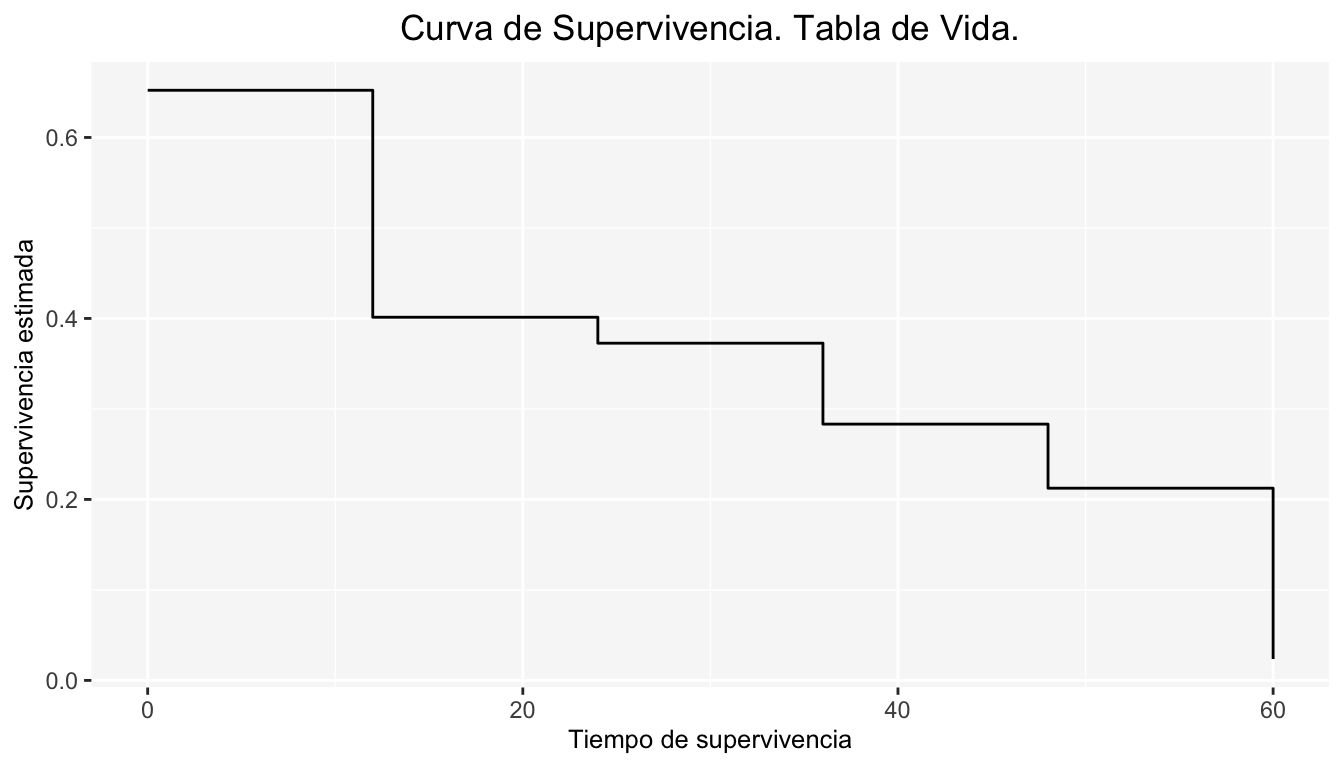
\includegraphics{_main_files/figure-latex/survival-actuar-example-1} 

}

\caption{Supervivencia estimada para los pacientes con myeloma múltiple con el método actuarial}\label{fig:survival-actuar-example}
\end{figure}

\hypertarget{estimador-producto-luxedmite-kaplan-meier}{%
\section{Estimador Producto-Límite (Kaplan-Meier)}\label{estimador-producto-luxedmite-kaplan-meier}}

El estimador producto-límite fue propuesto por Kaplan y Meier en 1958 como el estimador máximo-verosímil de la función de supervivencia.

El método de Kaplan-Meier calcula la supervivencia cada vez que un paciente muere. Da proporciones exactas de supervivencia debido a que utiliza tiempos de supervivencia precisos.

La característica distintiva del análisis con este método, es que la proporción acumulada que sobrevive se calcula para el tiempo de supervivencia individual de cada paciente, en contraste con la agrupación de los tiempos de supervivencia en intervalos hechos en la tabla de vida. Por esta razón es especialmente útil para estudios que utilizan un número pequeño de pacientes.

Este método asume que:

\begin{itemize}
\tightlist
\item
  Las personas que se retiran del estudio tienen un destino parecido a las que se quedan.
\item
  El periodo de tiempo durante el cual una persona entra en el estudio no tiene efecto independiente en la respuesta.
\end{itemize}

\hypertarget{construcciuxf3n-del-estimador-k-m}{%
\subsection{Construcción del Estimador K-M}\label{construcciuxf3n-del-estimador-k-m}}

Es natural pensar a \(T\) como una variable aleatoria continua, y por tanto, teóricamente no es posible tener observaciones iguales. No obstante, en la práctica los tiempos de supervivencia son medidos en escalas como: días, meses, años, etcétera; por lo que, hay posibilidad de tener observaciones repetidas. Por esta razón conviene modelar a \(T\) como una variable aleatoria discreta. La idea del estimador \emph{K-M} es la siguiente:

Sea \(T_{1}, T_{2},...,T_{n}\) una m.a. de una población discreta con soporte en \(\{u_{1}, u_{2},...\}\).

La muestra observada de \(T\) se puede representar como \((t_{i},\delta_{i})\) para \(i=1,2,...,n\) donde:

\[
\delta_{i} = \left\{
\begin{array}{ll}
0 & \mbox{si }  t_i \ es \ censurado\\
1 & \mbox{si }  t_{i} \ no \ es \ censurado
\end{array}
\right.
\]
Entonces la función de verosimilitud será:

\[ 
\mathscr{L} = \prod^{n}_{i=1}f(t_{i})^{\delta_{i}}S(t_{i})^{1-\delta_{i}} 
\]

Desarrollando la expresión anterior tenemos

\[
\mathscr{L} =\prod^{n}_{i=1}(h(u_{k})S(u_{k-1})\mathbb{1}_{t_{i}=u_{k}})^{\delta_{i}} (S(u_{k})\mathbb{1}_{k=max\{j:u_{j}\leq t_i\}})^{1-\delta_{i}}
\]

Sea

\[
\begin{split}
 & d_{k} = \sum_{i=1}^{n}\mathbb{1}_{(t_{i}=u_{k},\delta_{i}=1)} \mbox{  (numero de tiempos de fallo iguales a }u_{k}) \\
 & n_{k} = \sum_{i=1}^{n}\mathbb{1}_{(t_{i}\geq{u_{k}})} \mbox{ (numero de individuos en riesgo al tiempo } u_{k})
\end{split}
\]

\[
\Longrightarrow \mathscr{L} = \prod_{k} (h(u_k))^{d_k}(1-h(u_k))^{n_k-d_k}
\]

Ahora maximizamos la función de verosimilitud para \(h(u_k)\):

\[
\ln (\mathscr{L}) = \sum_{k}\{d_{k} \ln(h(u_{k}))+(n_{k}-d_{k}) \ln(1-h(u_{k}))\} 
\]

\[
\Longrightarrow \frac{\partial \ln (\mathscr{L})}{\partial h(u_{k})} = \frac{d_{k}}{h(u_{k})}-\frac{(n_{k}-d_{k})}{(1-h(u_{k}))} = 0
\]

despejando \(h(u_k)\) se tiene

\[
\therefore \hat{h}(u_{k}) = \frac{d_{k}}{n_{k}}
\]

Dado que los estimadores máximo-verosímiles cumplen con el principio de invarianza, y ocupando que \(S(t)=\prod_{k:u_{k}\leq t}(1-h(u_{k}))\) (visto anteriormente) tenemos:

\[
\hat S(t)=\prod_{k:u_{k}\leq t}\left(1-\frac{d_k}{n_k}\right)
\]

Y es así es como se deriva el estimador \emph{K-M}.

\textbf{Proposición:} \(\mathbb{E}[\hat{h}(u_k)] =h(u_k)\) (Insesgamiento).

\hypertarget{ejemplo-10}{%
\subsubsection*{Ejemplo}\label{ejemplo-10}}


Se obtuvieron los tiempos de remisión de 20 pacientes con osteosarcoma, a los que se trataba con 3 meses de quimioterapia después de amputación.

\begin{itemize}
\tightlist
\item
  11 pacientes recayeron a los 6, 8, 10, 11, 12, 13, 13, 22, 32, 34 y 36 meses.
\item
  8 pacientes se retiraron vivos al final del estudio contribuyendo 3, 7, 7, 11, 14, 16, 20 y 20 meses de observación, sin haber sufrido recaídas.
\item
  Un paciente rehusó continuar la terapia a los 11 meses y se retiró del estudio libre de enfermedad.
\end{itemize}

La siguiente tabla muestra la forma de estimar \(S(t)\) por el método \emph{K-M}:

\begin{table}
\centering
\begin{tabular}{cccccc}
\toprule
time & $d_j$ & $n_k$ & $c_k$ & $1-\frac{d_k}{n_k}$ & $S(t)$\\
\midrule
6 & 1 & 19 & 1 & 0.9473684 & 0.9473684\\
8 & 1 & 16 & 2 & 0.9375000 & 0.8881579\\
10 & 1 & 15 & 0 & 0.9333333 & 0.8289474\\
11 & 1 & 14 & 2 & 0.9285714 & 0.7697368\\
12 & 1 & 11 & 0 & 0.9090909 & 0.6997608\\
\addlinespace
13 & 2 & 10 & 0 & 0.8000000 & 0.5598086\\
22 & 1 & 4 & 4 & 0.7500000 & 0.4198565\\
32 & 1 & 3 & 0 & 0.6666667 & 0.2799043\\
34 & 1 & 2 & 0 & 0.5000000 & 0.1399522\\
36 & 1 & 1 & 0 & 0.0000000 & 0.0000000\\
\bottomrule
\end{tabular}
\end{table}

Y la gráfica de \(\hat S(t)\) es:

\begin{center}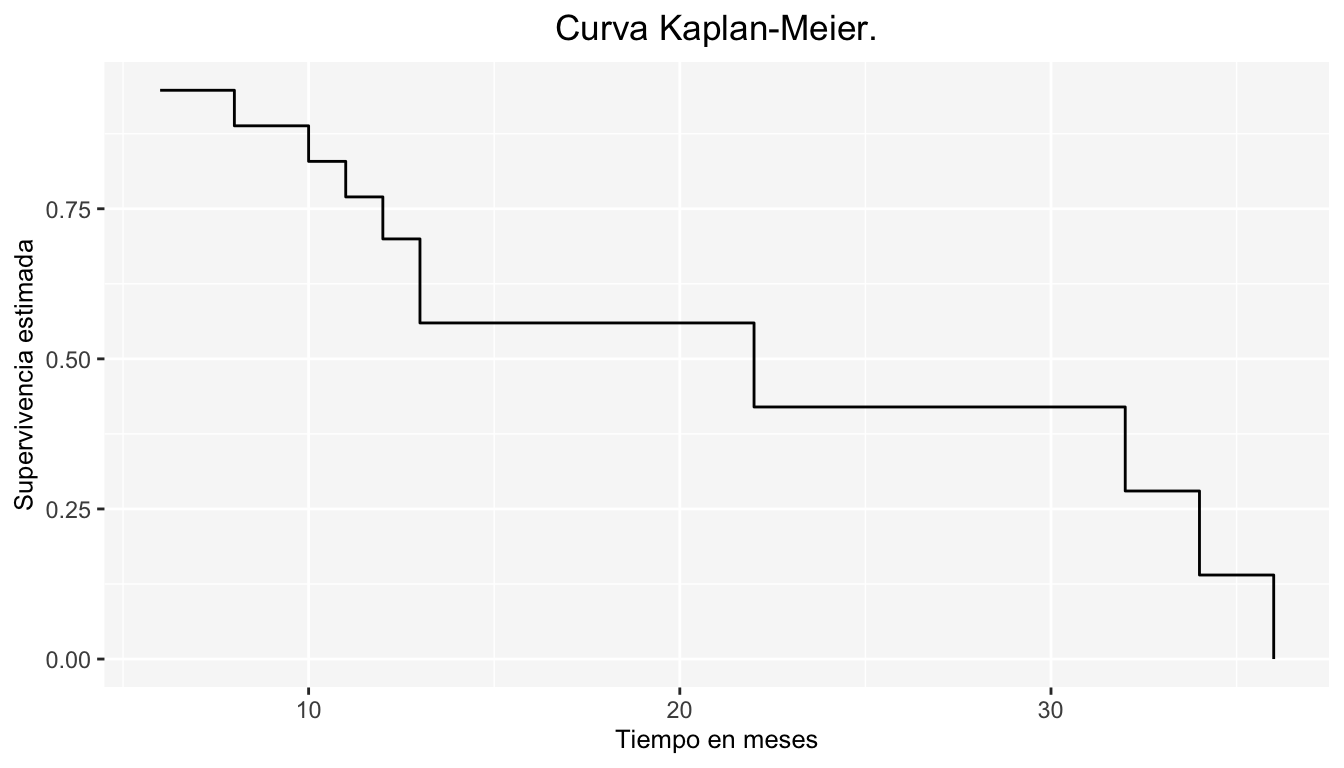
\includegraphics{_main_files/figure-latex/unnamed-chunk-25-1} \end{center}

\hypertarget{ejercicio}{%
\subsubsection*{Ejercicio}\label{ejercicio}}


Suponga que disponemos de los datos de supervivencia de 10 pacientes que han sido aleatoriamente asignados a los tratamientos A y B.

\begin{itemize}
\tightlist
\item
  A: 3, 5, 7, 9+, 18
\item
  B: 12, 19, 20, 20+, 33+
\end{itemize}

Construya la función de supervivencia para cada tratamiento y grafíquelas. ¿Qué se puede decir de los tratamientos a partir de las gráficas?

\hypertarget{algunas-estimaciones-sobre-modelos-no-paramuxe9tricos}{%
\chapter{Algunas Estimaciones sobre Modelos No Paramétricos}\label{algunas-estimaciones-sobre-modelos-no-paramuxe9tricos}}

Cuando se emplean los modelos no paramétricos, es necesario hacer inferencia más allá de la estimación puntual. Para tal propósito, conocer la varianza de algunos estimadores de interés, resulta de gran ayuda.

\hypertarget{estimaciuxf3n-de-la-varianza-para-el-estimador-de-st}{%
\section{\texorpdfstring{Estimación de la Varianza para el Estimador de \(S(t)\)}{Estimación de la Varianza para el Estimador de S(t)}}\label{estimaciuxf3n-de-la-varianza-para-el-estimador-de-st}}

\hypertarget{tabla-de-vida}{%
\subsection{Tabla de Vida}\label{tabla-de-vida}}

Para la tabla de vida se tienen los siguientes resultados:

\[
\begin{array}{ll}
\hat{q_j} = \frac{d_{j}}{n_{j}-\frac{c_{j}}{2}} &  \hat{S_{j}}=\prod_{i=1}^{j}\left(1-\frac{d_{i}}{n_{i}-\frac{c_{i}}{2}}\right)\\
\end{array}
\]

Entonces un estimador de la varianza para \(\hat{S_j}\) es:

\[
 \hat{Var}(\hat{S}_{j}) = \hat{S}_{j}^2\sum_{i = 1}^{j}\frac{\hat{q_i}}{\hat{p_i}(n_{i}-\frac{c_{i}}{2})}
\]

Si deseamos obtener intervalos de confianza puntuales para \(S(t)\), podemos partir de la distribución asintótica de \(\hat{S_j}\):

\[
\hat{S}_j \sim N(S_{j}, \hat{Var}(\hat{S_{j}}))
\]

De donde, un intervalo de confianza para \(S(t_j)\) al \((1-\alpha)*100\%\) es:

\[
\hat S_j \pm Z_{1-\frac{\alpha}{2}} \sqrt{\hat{Var}(\hat S_j)}
\]

\hypertarget{kaplan-meier}{%
\subsection{Kaplan-Meier}\label{kaplan-meier}}

Partiendo de que

\[
\hat{S}(t) = \prod_{k:u_k \leq t}(1-h_{k})
\]

Si aplicamos \(\ln\) tenemos:

\[
\ln(\hat{S(t)}) = \sum_{k:u_k \leq t} \ln(1-h_k)
\]

\[
\Longrightarrow Var(\ln(\hat{S}(t))) = \sum_{k:u_k \leq t} Var(\ln(1-h_k))
\]

Desarrollando con series de Taylor (método Delta) se obtiene:

\[
Var(\hat{S}(t)) = \hat{S}^2(t)\sum_{k:u_k \leq t}\frac{Var(\hat{h}_k)}{(1-\hat{h}_{k})^2}
\]

Uno de los \textbf{estimadores} más comunes para \(Var(\hat{S}(t))\) es el \textbf{estimador de Greenwood}; éste supone que el número de individuos que sobreviven a lo largo del intervalo que empieza en \(t_j\) tiene una distribución \emph{Binomial} con parámetros \(n_j\) y \(p_j\) (\(p_j\) es la verdadera probabilidad de supervivencia a lo largo del intervalo). De manera que, el estimador Greenwood es:

\[
\hat{Var}(\hat{S}(t)) \approx \hat{S}^2(t) \sum_{j:t_{j}\leq t}\frac{d_{j}}{n_{j}(n_{j}-d_{j})}
\]

\begin{itemize}
\item
  El estimador del error estándar será: \(\sqrt{\hat{Var}(\hat{S}(t))}\).
\item
  Cuando \(n\rightarrow\infty\), \(\hat{S}(t)\) tiene una distribución normal: \(\hat{S}(t)\sim N(S(t), Var(\hat{S}(t)))\).
\item
  El intervalo puntual al \((1-\alpha)*100\%\) de confianza para \(S(t_{0})\) será: \(\hat{S}(t_{0}) \pm Z_{1-\alpha/2} \sqrt{\hat{Var}(\hat{S}(t_0))}\)\footnote{Posiblemente al realizar las cuentas, como en el ejemplo que se encuentra en esta sub sección, se obtengan valores negativos en alguno de los límites inferiores del intervalo de confianza. Esto es porque la expresión matemática del intervalo de confianza permite este tipo de valores, pero al tratarse de una función de supervivencia \(S(t)\) su rango serán valores en \([0,1]\), por lo que, por convención, se coloca el valor 0 cuando se tiene un número negativo.}.
\end{itemize}

Para este último punto, pueden existir ocasiones en las que el intervalo de confianza se encuentre fuera del rango \([0,1]\), por lo que existen diferentes aproximaciones para resolver dicho problema. Una de ellas es mejorando la aproximación a la distribución normal (ya que se menciono previamente que : \(\hat{S}(t)\sim N(S(t), Var(\hat{S}(t)))\)) utilizando la transformación \(log-log\), obteniendo así la siguiente expresión:

\[
\hat{S}(t_{0}) \pm e^{Z_{1-\alpha/2} \frac{\sqrt{\hat{Var}(\hat{S}(t_0))}}{\hat{S}(t_{0})\ln(\hat{S}(t_{0}))}}
\]

Otra alternativa es utilizando una transformación logarítmica para obtener lo siguiente

\[
\exp\left(\ln(\hat{S}(t_{0})) \pm Z_{1-\alpha/2} \frac{\sqrt{\hat{Var}(\hat{S}(t_0))}}{\hat{S}(t_{0})}\right)
\]

\hypertarget{ejercicio-1}{%
\subsubsection*{Ejercicio}\label{ejercicio-1}}


Un estudio consistió en medir el tiempo(en meses) en que los pacientes desarrollaron un cierto tipo de tumor. Los resultados que se obtuvieron fueron:

\[
10,13^+,18^+,19,23^+,30,36,38^+,54^+,56^+,59,75,93,97,104^+,107,107^+,107^+
\]

La siguiente tabla muestra \(\hat S(t)\) por el método de \emph{K-M}, además de los intervalos de confianza puntuales utilizando el estimador de \emph{Greenwood}:

\begin{table}
\centering
\begin{tabular}{cccccccc}
\toprule
time & $d_k$ & $n_k$ & $c_k$ & $S(t)$ & std error & Lower\_95\% & Upper\_95\%\\
\midrule
10 & 1 & 18 & 0 & 0.9444444 & 0.0539903 & 0.8386254 & 1.0000000\\
19 & 1 & 15 & 2 & 0.8814815 & 0.0789892 & 0.7266655 & 1.0000000\\
30 & 1 & 13 & 1 & 0.8136752 & 0.0977770 & 0.6220358 & 1.0000000\\
36 & 1 & 12 & 0 & 0.7458689 & 0.1106702 & 0.5289593 & 0.9627785\\
59 & 1 & 8 & 3 & 0.6526353 & 0.1303197 & 0.3972133 & 0.9080573\\
\addlinespace
75 & 1 & 7 & 0 & 0.5594017 & 0.1411673 & 0.2827189 & 0.8360845\\
93 & 1 & 6 & 0 & 0.4661681 & 0.1451991 & 0.1815830 & 0.7507531\\
97 & 1 & 5 & 0 & 0.3729345 & 0.1429930 & 0.0926734 & 0.6531955\\
107 & 1 & 3 & 3 & 0.2486230 & 0.1392472 & 0.0000000 & 0.5215425\\
\bottomrule
\end{tabular}
\end{table}

La gráfica correspondiente es:

\begin{center}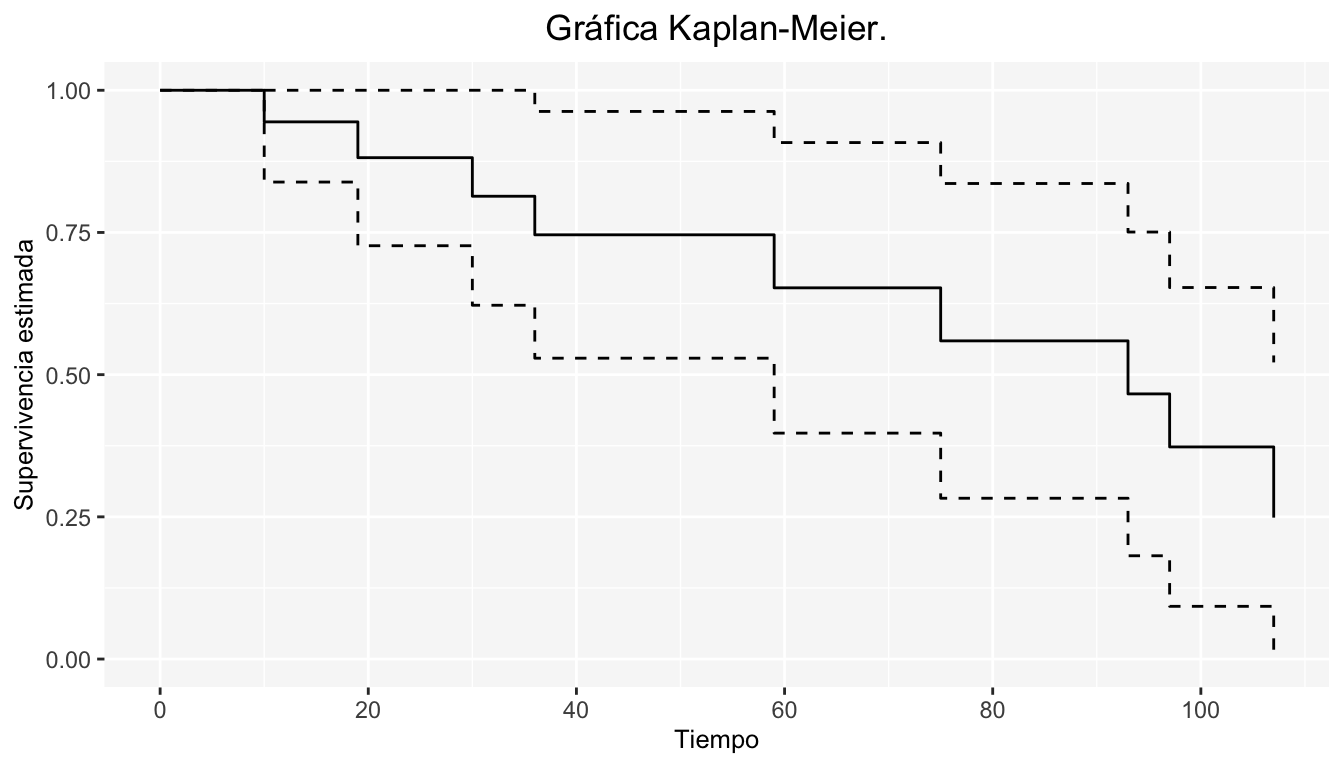
\includegraphics{_main_files/figure-latex/unnamed-chunk-27-1} \end{center}

\hypertarget{estimadores-de-la-funciuxf3n-de-riesgo-acumulada}{%
\section{Estimadores de la Función de Riesgo Acumulada}\label{estimadores-de-la-funciuxf3n-de-riesgo-acumulada}}

Recordemos que:

\[
H(t)=-log(S(t)) 
\]

Entonces podemos estimar \(H(t)\) de una manera sencilla (\(\hat{S}(t)\) es obtenido por \emph{K-M}):

\[
\hat{H_1}(t) = -log(\hat{S}(t))
\]

No obstante, una alternativa para conocer \(H(t)\) es utilizar el \textbf{estimador Nelson-Aalen}. Este estimador resulta útil primordialmente en el análisis de datos para la selección entre modelos paramétricos para el tiempo de fallo \(T\), además proporciona un estimador para \(h(t)\). El estimador \emph{Nelson-Aalen} asume que \(H(t)\) es la suma de riesgos, esto es:

\[
H(t)=\sum_{j:u_{j}\leq t} h_j
\]

Entonces el estimador de \(H(t)\) será:

\[
\hat{H_2}(t)=\sum_{j:u_{j}\leq t} \hat h_j=\sum_{j:u_{j}\leq t}\frac{d_j}{n_j}
\]

Observe que si tomamos \(\hat H_2(t)\), podemos estimar de otra manera a \(S(t)\). Es decir, \(S(t)\), usando \textbf{Nelson-Aalen}, se obtiene el estimador \emph{\textbf{Fleming-Harrington}}, el cual es:

\[
\hat{S_2}(t) = exp\{-\hat{H_2}(t)\} = exp\left\{-\sum_{j:u_{j}\leq t}\frac{d_j}{n_j}\right\}
\]

Un estimador de la varianza de \(\hat{H_2}(t)\) es:

\[
\hat{Var}(\hat{H_2}(t)) = \sum_{j:t_{j}\leq t}\frac{d_j}{n_{j}^{2}}
\]

Y el intervalo de confianza puntual al \((1-\alpha)*100\%\) para \({H_2}(t_0)\) es:

\[
\hat{H_2}(t_{0}) \pm Z_{1-\alpha/2} \frac{\sqrt{\hat{Var}\{\hat{H_2}(t)\}}}{\hat{H_2}(t_{0})}
\]

\hypertarget{ejemplo-11}{%
\subsubsection*{Ejemplo}\label{ejemplo-11}}


Siguiendo con el ejemplo anterior, que mide el tiempo (en meses) en que los pacientes desarrollaron un cierto tipo de tumor.

La tabla muestra \(\hat S(t)\) por el método de \emph{K-M}, entonces podemos calcular \(\hat {H}_1(t)=-log(\hat S(t))\). Y por otro lado usar el estimador Nelson-Aalen para obtener \(\hat{H}_2(t)\).

\begin{table}
\centering
\begin{tabular}{ccccccc}
\toprule
time & $d_k$ & $n_k$ & $c_k$ & $S(t)$ & $H_1(t)$ & $H_2(t)$\\
\midrule
10 & 1 & 18 & 0 & 0.9444444 & 0.0571584 & 0.0555556\\
19 & 1 & 15 & 2 & 0.8814815 & 0.1261513 & 0.1222222\\
30 & 1 & 13 & 1 & 0.8136752 & 0.2061940 & 0.1991453\\
36 & 1 & 12 & 0 & 0.7458689 & 0.2932054 & 0.2824786\\
59 & 1 & 8 & 3 & 0.6526353 & 0.4267368 & 0.4074786\\
\addlinespace
75 & 1 & 7 & 0 & 0.5594017 & 0.5808874 & 0.5503358\\
93 & 1 & 6 & 0 & 0.4661681 & 0.7632090 & 0.7170024\\
97 & 1 & 5 & 0 & 0.3729345 & 0.9863526 & 0.9170024\\
107 & 1 & 3 & 3 & 0.2486230 & 1.3918177 & 1.2503358\\
\bottomrule
\end{tabular}
\end{table}

\hypertarget{estimaciuxf3n-puntual-de-la-media}{%
\section{Estimación Puntual de la Media}\label{estimaciuxf3n-puntual-de-la-media}}

Puede ser de interés estudiar algunos parámetros poblacionales que dependen de la función de supervivencia. Por ejemplo: la media, la mediana y cualquier cuantil o percentil.

Hemos visto en la sección \ref{media} que:

\[
\mu = \int_{0}^{\infty}S(t)dt
\]

Entonces podemos reemplazar \(S(t)\) con el estimador de \(\hat{S}(t)\)(obtenido por \emph{K-M}), por lo que:

\[
\hat{\mu}=\int_{0}^{\infty}\hat{S}(t)dt
\]

\textbf{Observación:} El estimador será apropiado si la observación más grande del conjunto de datos es un tiempo de falla y \textbf{NO} una observación censurada.

Si la última observación(la más grande) es una observación censurada, entonces \(\hat{\mu}\) se calcula como:

\[
\hat{\mu}_{\tau} =\int_{0}^{\tau}\hat{S}(t)dt
\]

Donde \(\tau\) es el valor que determina el tiempo más grande al que una persona puede sobrevivir.

Un estimador de la varianza de \(\hat{\mu}_{\tau}\) con \(t_{1}, t_{2},...,t_{k}\) tiempos de fallo observados, es:

\[
\hat{Var}(\hat{\mu_\tau}) = \sum_{i = 1}^{k}\left\{\int_{t_i}^{\tau}\hat{S}(t)dt\right\}^2 \cdot \frac{d_{i}}{n_{i}(n_{i}-d_{i})}
\]

El intervalo al \((1-\alpha)100\%\) de confianza para \(\mu_\tau\) es:

\[
\hat\mu_{\tau} \pm Z_{1-\alpha/2}\sqrt{\hat{Var}(\hat\mu_\tau)}
\]

\textbf{NOTA:} Es importante que, cuando se esté calculando la media de supervivencia \(\hat\mu_{\tau}\), se verifique que el último valor no sea censurado y se observe en qué intervalo se está calculando la media.

\hypertarget{estimaciuxf3n-de-cuantiles}{%
\section{Estimación de Cuantiles}\label{estimaciuxf3n-de-cuantiles}}

Recordemos que los cuantiles de orden \(p\), \(t_p\), es el mínimo valor \(t\) tal que \(S(t)\leq 1-p\). Usando el estimador \(\hat{S}(t)\) obtenido por \emph{K-M}, tenemos:

\[
\hat{t}_p = inf\{t:\hat{S}(t)\leq 1-p\}
\]

Por lo que, si deseamos calcular la \textbf{mediana estimada}:

\[
\hat{t}_{0.5} = inf\{t:\hat{S}(t)\leq 0.5\}
\]

\hypertarget{bandas-de-confianza-para-la-funciuxf3n-de-supervivencia}{%
\section{Bandas de Confianza para la Función de Supervivencia}\label{bandas-de-confianza-para-la-funciuxf3n-de-supervivencia}}

Deseamos encontrar dos v.a. \(L(t)\) y \(U(t)\) tales que:

\[
\begin{array}{ll}
\mathbb{P}(L(t)\leq S(t)\leq U(t)) = 1-\alpha & \forall t_{L}\leq t\leq t_{U}\\
\end{array}
\]

Entonces \([L(t), U(t)]\) serán las bandas al \((1-\alpha)*100\%\) de confianza de \(S(t)\). Puede usted decir ¿cuál es la diferencia entre \emph{bandas de confianza} e \emph{intervalos de confianza puntuales}?

Hay dos métodos de aproximación para las bandas de confianza. La primera aproximación fue propuesta por \emph{Nair} \citep{nair1984confidence} y esencialmente proporciona límites de confianza que son proporcionales a los intervalos de confianza puntuales, estas bandas son llamadas \emph{bandas de probabilidad iguales} o \emph{bandas EP}\footnote{Tanto para estas bandas como las de Hall \& Wellner se consideran los \(D\) eventos distintos del tiempo \(t_1<t_2<\cdots<t_D\); \(t_L<t_U\) el rango de tiempo para las bandas de confianza, por lo que \(t_U\) es menor o igual al evento de tiempo más grande. \(t_L\), en este caso es más grande o igual al tiempo de evento más pequeño y para ambas bandas se tiene que \(\alpha_L = \frac{n\sigma^2_S(t_L)}{1+n\sigma^2_S(t_L)} \mbox{ y } \alpha_U = \frac{n\sigma^2_S(t_U)}{1+n\sigma^2_S(t_U)}\).
  Las bandas EP al \(100(1-\alpha)\%\) están dadas por \[\hat{S}(t)-e_{\alpha}(\alpha_L, \alpha_U)\hat{S}(t)\sigma_S(t)\leq S(t)\leq\hat{S}(t)+e_{\alpha}(\alpha_L, \alpha_U)\hat{S}(t)\sigma_S(t)\] para todos los \(t_L\leq t\leq t_U\), donde \(e_{\alpha}(\alpha_L, \alpha_U)\) es un cuantil tal que \(\alpha = \mathbb{P}\left(\sup\limits_{\alpha_L\leq u\leq \alpha_U}\frac{|W^0(u)|}{[u(1-u)]^{1/2}}> e_{\alpha}\left(\alpha_L, \alpha_U\right)\right)\) donde \(W^0(u)\) es un \href{https://en.wikipedia.org/wiki/Brownian_bridge}{puente browninano} con \(0\leq u\leq1\) y \(\hat{S}(t)\sigma_S(t)\) se derivada del estimador de Greenwood.}. Caso contrario, la segunda aproximación, propuesta por \href{http://www.ressources-actuarielles.net/EXT/ISFA/1226.nsf/0/b163cbaba7cf2db9c125776b004d3573/\%24FILE/Hall_Wellner_1980.pdf}{\emph{Hall} y \emph{Wellner}}\footnote{Las bandas Hall and Wellner al \(100(1-\alpha)\%\) están dadas por \(\hat{S}(t)-h_{\alpha}(\alpha_L, \alpha_U)\sqrt{n}\left[1+n\sigma^2_S(t)\right]\hat{S}(t)\leq S(t)\leq\hat{S}(t)+h_{\alpha}(\alpha_L, \alpha_U)\sqrt{n}\left[1+n\sigma^2_S(t)\right]\hat{S}(t)\) para todos los \(t_L\leq t\leq t_U\) donde los valores críticos \(h_\alpha(\alpha_L, \alpha_U)\) esta dado por \(\alpha = \mathbb{P}\left(\sup\limits_{\alpha_L\leq u\leq \alpha_U}|W^0(u)|> h_\alpha\left(\alpha_L, \alpha_U\right)\right)\). En este caso, \(t_L\) puede ser cero. Se puede consultar más sobre estas expresiones en el siguiente \href{https://documentation.sas.com/?cdcId=pgmsascdc\&cdcVersion=9.4_3.4\&docsetId=statug\&docsetTarget=statug_lifetest_details11.htm\&locale=ko}{enlace}.} \citep{hall1980confidence}, establece bandas no proporcionales a los intervalos de confianza puntuales.

Nuestro interés es obtener las bandas de confianza para \(S(t)\); afortunadamente hoy en día se cuenta con software que nos ayuda en dicha tarea, específicamente en \textbf{R} es sencillo obtenerlo.

\hypertarget{diagnuxf3stico-para-el-uso-de-modelos-paramuxe9tricos}{%
\section{Diagnóstico para el Uso de Modelos Paramétricos}\label{diagnuxf3stico-para-el-uso-de-modelos-paramuxe9tricos}}

Si existe la necesidad de encontrar un modelo paramétrico que ajuste ``bien'' a los datos, se pueden emplear algunos métodos gráficos que nos den algunos \emph{indicios} sobre la posible \emph{distribución} de los datos. Tales indicios pueden ser proporcionados por los métodos no paramétricos.

\hypertarget{gruxe1ficas-de-las-funciones-de-supervivencia}{%
\subsection{Gráficas de las Funciones de Supervivencia}\label{gruxe1ficas-de-las-funciones-de-supervivencia}}

Se conoce la función de supervivencia paramétrica \(S(t ;\theta)\) y se tiene un estimador \(\hat \theta\). Si el modelo paramétrico es \emph{adecuado} entonces \(S(t ;\hat {\theta})\) y \(\hat S(t)\)(estimada por \emph{K-M}) deben ser \emph{similares}.

\hypertarget{ejemplo-12}{%
\subsubsection*{Ejemplo}\label{ejemplo-12}}


Se tienen los siguientes tiempos de supervivencia:

\[
8,5,10^+,1,3,18,22,15,25^+,19
\]

Se desea saber si estos datos ajustan a un modelo \emph{exponencial} con \(\lambda =0.06\). Realizamos las gráficas de supervivencia:

\begin{center}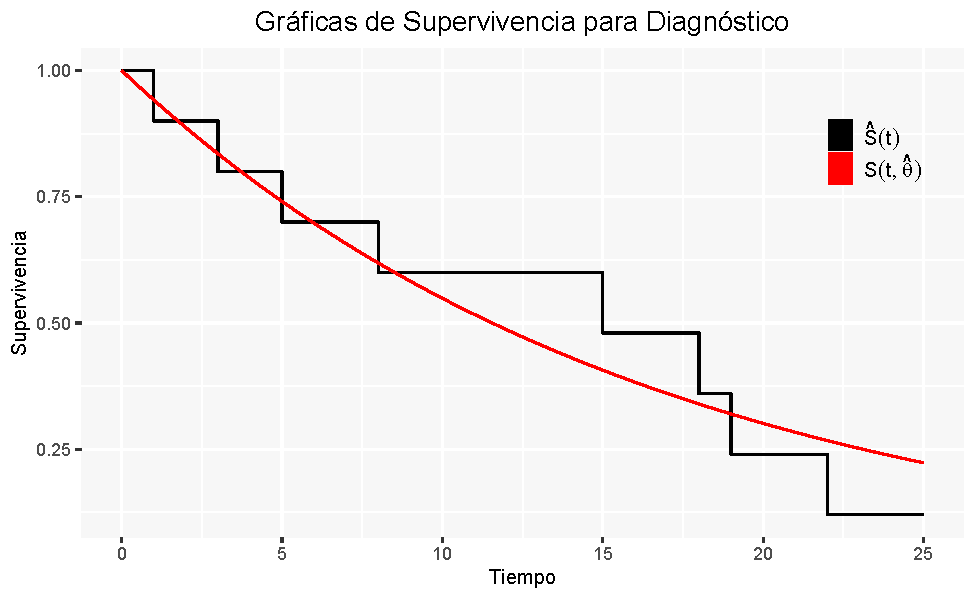
\includegraphics{_main_files/figure-latex/unnamed-chunk-29-1} \end{center}

De acuerdo a la gráfica anterior, ¿Existe algún indicio de que los datos siguen una distribución exponencial con \(\lambda =0.06\)?

\hypertarget{gruxe1fica-p-p}{%
\subsection{\texorpdfstring{Gráfica \(P-P\)}{Gráfica P-P}}\label{gruxe1fica-p-p}}

Si el modelo paramétrico es adecuado entonces los puntos:

\[
\left(S(t_j ;\hat{\theta}),\hat S(t_j)\right)
\]

Deberán caer en la recta identidad (\(\hat S(t_j)\) es estimada por \emph{K-M}). Es llamada \emph{gráfica \(P-P\)} pues se gráfica \emph{Probabilidad vs Probabilidad}.

\hypertarget{ejemplo-13}{%
\subsubsection*{Ejemplo}\label{ejemplo-13}}


Tomando los datos del ejemplo anterior, queremos ver si los datos se distribuyen posiblemente exponencial con \(\lambda =0.06\). Si hacemos la gráfica \emph{P-P} se tiene:

\begin{center}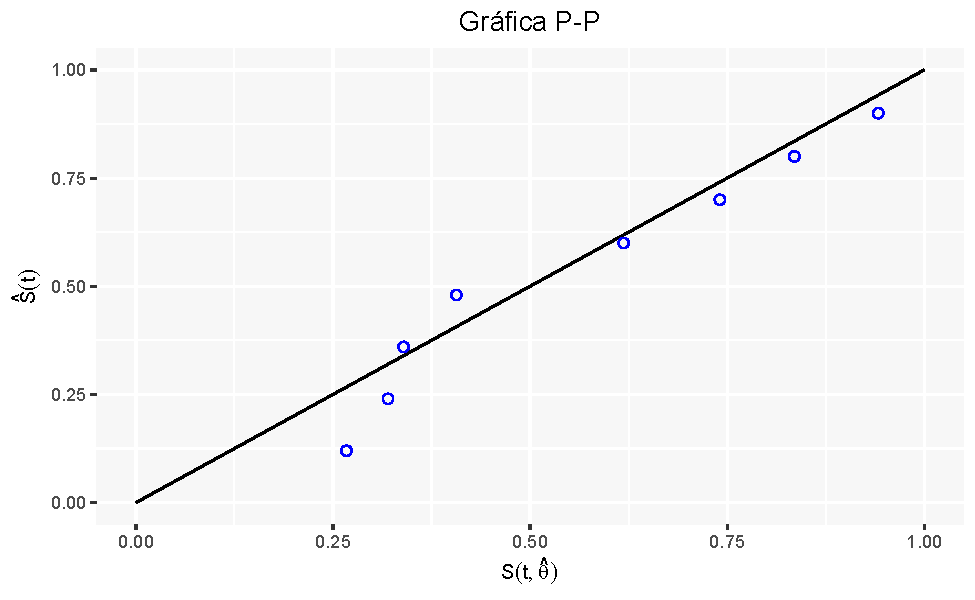
\includegraphics{_main_files/figure-latex/unnamed-chunk-30-1} \end{center}

De acuerdo a la gráfica \emph{\(P-P\)}, ¿Es el modelo exponencial con \(\lambda=0.06\) adecuado a los datos?

\hypertarget{gruxe1fica-q-q}{%
\subsection{\texorpdfstring{Gráfica \(Q-Q\)}{Gráfica Q-Q}}\label{gruxe1fica-q-q}}

La \emph{gráfica \(Q-Q\)} consiste en graficar diversos cuantiles de los \textbf{datos} \emph{vs} diversos cuantiles del modelo paramétrico propuesto. Si el modelo teórico propuesto es ``adecuado'' a los datos entonces la gráfica será cercana a la función identidad.

A continuación se muestra un ejemplo de la gráfica \(Q-Q\):

\begin{center}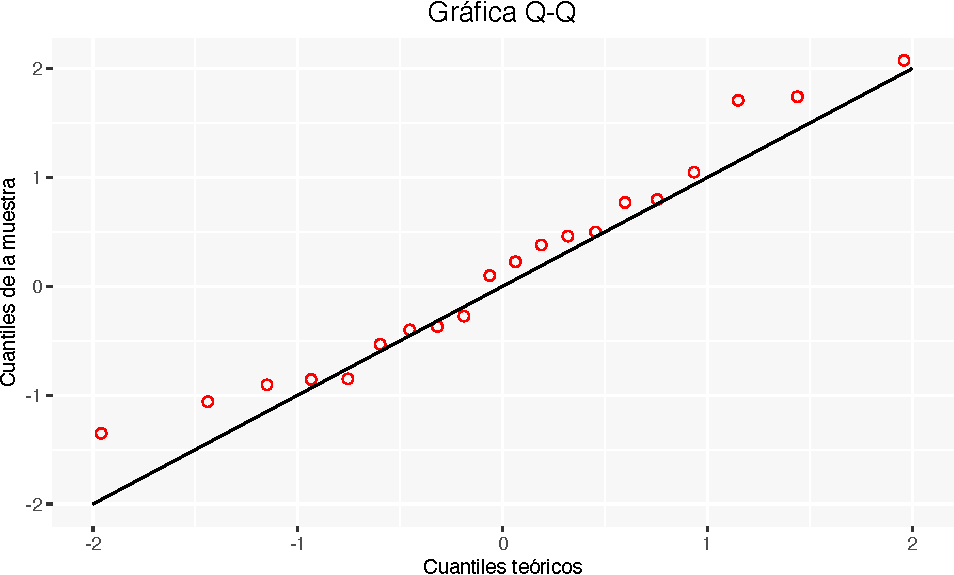
\includegraphics{_main_files/figure-latex/unnamed-chunk-31-1} \end{center}

\hypertarget{linearizaciuxf3n-de-la-funciuxf3n-de-supervivencia}{%
\subsection{Linearización de la Función de Supervivencia}\label{linearizaciuxf3n-de-la-funciuxf3n-de-supervivencia}}

Cuando tenemos un modelo paramétrico \(S(t;\theta)\) pero no conocemos \(\hat{\theta}\) podemos hacer \emph{linearización de la función de supervivencia}. Es decir, si existen \(g_1\) y \(g_2\) tales que \(g_1\{S(t;\theta)\}\) es una función \emph{lineal} de \(g_2(t)\) entonces podemos graficar \(g_1(\hat{S}(t))\) \emph{vs} \(g_2(t)\). Y si la familia paramétrica es adecuada, la gráfica se aproxima a una linea recta. Para este método gráfico se utiliza el estimador \textbf{Nelson-Aalen} para \(\hat S(t)\).

\hypertarget{modelo-exponencial-2}{%
\subsubsection*{Modelo Exponencial}\label{modelo-exponencial-2}}


Tenemos que:

\[
S(t)=e^{-\lambda t}
\]

\[
\Longrightarrow log\{S(t)\}=-\lambda t  
\]

De manera que \(g_1=log\{S(t)\}\) y \(g_2=t\). Entonces debemos graficar \(log(\hat S(t))\) \emph{vs} \(t\), y si los datos se ajustan a un modelo exponencial, dicha gráfica debe ser aproximadamente una linea recta con pendiente \(-\lambda\).

\hypertarget{ejemplo-14}{%
\subsubsection*{Ejemplo}\label{ejemplo-14}}


Consideremos los datos: \(8,5,10^+,1,3,18,22,15,25^+,19\), veamos si se pueden ajustar posiblemente a un modelo exponencial a través de la gráfica de linearización. Entonces tenemos:

\begin{center}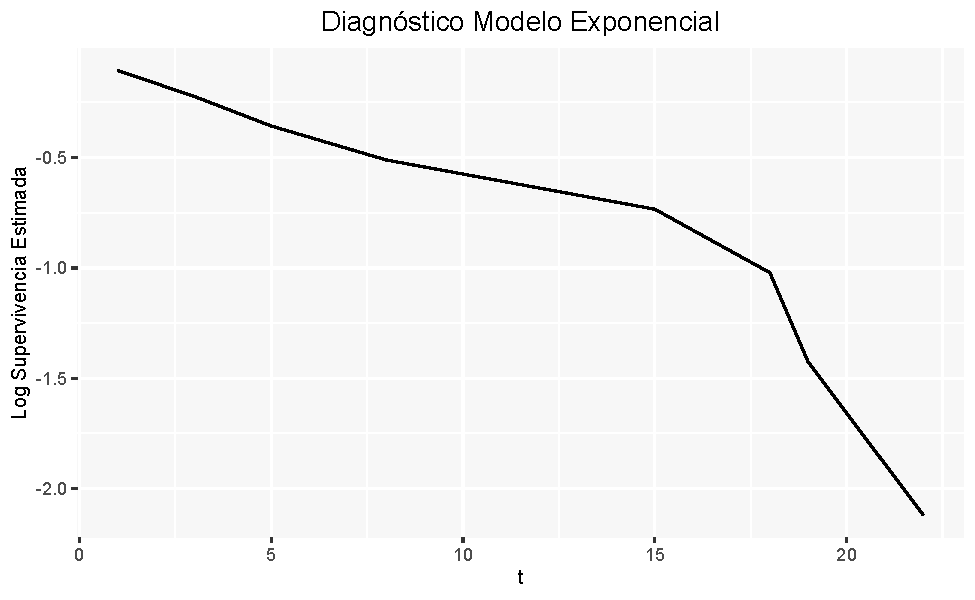
\includegraphics{_main_files/figure-latex/unnamed-chunk-32-1} \end{center}

¿Qué puede decir a partir de la gráfica anterior?, ¿Puede asumirse que los datos se ajustan a un modelo exponencial?

\hypertarget{modelo-weibull-2}{%
\subsubsection*{Modelo Weibull}\label{modelo-weibull-2}}


Para el modelo Weibull tenemos que:

\[
S(t)=e^{-(\lambda t)^{\gamma}}
\]

\[
\Longrightarrow -log\{S(t)\}=(\lambda t)^{\gamma}
\]

\[
\Longrightarrow log\{-log\{S(t)\}\}=\gamma (log(\lambda)+log(t))
\]

Entonces \(g_1=log\{-log\{S(t)\}\}\) y \(g_2=log(t)\). Por lo que debemos graficar \(log\{-log\{\hat S(t)\}\}\) \emph{vs} \(log(t)\), y si los datos se ajustan a un modelo Weibull, la gráfica debe ser aproximadamente una linea recta con intercepto \(\gamma log(\lambda)\) y pendiente \(\gamma\).

\hypertarget{modelo-log-loguxedstico-1}{%
\subsubsection*{Modelo Log-Logístico}\label{modelo-log-loguxedstico-1}}


La función de supervivencia es:

\[
S(t)=(1+\lambda t^{\alpha})^{-1}
\]

\[
\Longrightarrow -log\{S(t)\}=log(1+\lambda t^{\alpha})
\]

\[
\Longrightarrow log\{exp\{-log\{S(t)\}\}-1\}=log(\lambda)+\alpha log(t)
\]

La gráfica de diagnóstico es: \(log\{exp\{-log\{\hat S(t)\}\}-1\}\) \emph{vs} \(log(t)\). Si el modelo Log-Logístico es adecuado a los datos, entonces la gráfica es aproximadamente una linea recta con intercepto \(log(\lambda)\) y pendiente \(\alpha\).

\hypertarget{modelo-log-normal-1}{%
\subsubsection*{Modelo Log-Normal}\label{modelo-log-normal-1}}


Para este modelo, la gráfica que debemos emplear para el diagnóstico es \(\Phi^{-1}[1-exp(-log(\hat S(t)))]\) \emph{vs} \(log(t)\), donde \(\Phi^{-1}\) son los cuantiles de una \emph{Normal estándar}. Una linea recta(aproximadamente) indica una posible distribución Log-Normal en los datos.

Los métodos gráficos que hemos visto son una herramienta que proporcionan indicios sobre la posible distribución de los datos(si nuestro interés es encontrar un modelo paramétrico). Evidentemente una gráfica no \textbf{demuestra nada} por lo que tendríamos que realizar pruebas formales de \textbf{bondad de ajuste} (pruebas que consideren la censura y/o truncamiento).

\hypertarget{pruebas-de-hipuxf3tesis}{%
\chapter{Pruebas de Hipótesis}\label{pruebas-de-hipuxf3tesis}}

Las pruebas de hipótesis juegan un papel importante en la inferencia estadística. En el contexto del análisis de supervivencia, resulta primordial comparar poblaciones en cuanto a sus funciones de supervivencia, pues de ello podemos saber, por ejemplo, la \emph{eficacia} de un tratamiento respecto a otro, los tiempos de aparición de un tumor en dos grupos, entre otras cosas.

El objetivo de la comparación de poblaciones en el análisis de supervivencia es similar a aquellos procedimientos diseñados para comparar estadísticos provenientes de muestras independientes, como la \emph{prueba t}, la \emph{prueba de los signos}, la \emph{prueba U de Mann-Whitney}(1947), la \emph{prueba de Kruskal-Wallis}(1952), etcétera. Todas estas pruebas de comparación se utilizan para evaluar diferencias entre estadísticos que han sido estimados basados en la información que se obtiene de subgrupos poblacionales independientes entre si. No obstante, dichas pruebas \textbf{no consideran la censura} en los datos, y por esta razón se imposibilita su aplicación ``directa'' en datos de supervivencia.

Las pruebas más utilizadas para comparar funciones de supervivencia, las cuales consideran la censura en los datos, son: la \emph{prueba Log-Rank} propuesta por Mantel-Haenszel(1959), la \emph{prueba generalizada de Wilcoxon} propuesta por Gehan(1965), la \emph{prueba de Peto-Peto}(1972), la \emph{prueba de Tarone-Ware}(1977), la \emph{prueba de Harrington-Fleming}(1982) que generaliza parte de las pruebas anteriores y una versión más general propuesta por Fleming et al.~(1987). En esta sección veremos la prueba de \emph{Log-Rank} y la prueba generalizada de \emph{Wilcoxon}, que esencialmente son la misma salvo una ponderación.

\hypertarget{comparaciuxf3n-de-1-poblaciuxf3n}{%
\section{Comparación de 1 población}\label{comparaciuxf3n-de-1-poblaciuxf3n}}

Suponiendo que la tasa de riesgo real en la población estudiada es \(h(t)\), el objetivo en esta prueba es determinar, estadisticamente, si la tasa de riesgo \(h_0(t)\), la cual está completamente especificado en el intervalo \((0,\tau)\), es adecuada para las observaciones a tratar para un tiempo fijo \(\tau\), es decir:

\[
\begin{array}{ccc}
H_0:h(t) = h_0(t)\ \forall \ t\leq \tau&vs& H_a:h(t) \neq h_0(t);\ \mbox{ p.a } \ t\leq \tau
\end{array}
\]

Recordando que el estimador de la función de riesgo acumulado es \(\hat{H}_2(t) = \sum_{t_{i}\leq t}\frac{d_i}{n_i}\), entonces \(\frac{d_i}{n_i}\) es un estimador de la tasa de riesgo en \(t_i\).

Cuando la hipótesis nula es cierta, el valor esperado de la tasa de riesgo en \(t_i\) es \(h_0(t_i)\). Ahora, sea \(\omega(t)\) la función de pesos tal que \(\omega(t) = 0\) si \(n_t = 0\), es decir que no se otorga algún peso cuando no hay elementos en dicho tiempo.

Considerando el clásico estadístico de prueba \(Z(\tau) = O(\tau)-\mathbb{E}(\tau)\) (elementos observados menos esperados) \footnote{Ver el parecido con el estadístico utilizado en pruebas de independencia.} y considerando que \(D\) es el número de tiempos en la muestra, se tiene lo siguiente:

\[
Z(\tau) = O(\tau)-\mathbb{E}(\tau) = \sum_{i = 1}^D\omega(ti)\frac{d_i}{n_i}-\int_0^{\tau}\omega(s)h_0(s)ds
\]
Sólo para confirmar, \(O(\tau)\) representa el número de eventos al tiempo \(\tau\). Cuando \(H_0\) es cierta

\[
Var(Z(\tau)) = \int_0^{\tau}\omega^2(s)\frac{h_0(s)}{n_s}ds
\]

Entonces, para muestras grandes el siguiente estadístico tiene una distribución \(\chi^2_{(1)}\)\footnote{¿Qué distribución de conteo tiene la misma varianza que su media?}.

\[
T = \frac{[Z(\tau)]^2}{Var(Z(\tau))}\sim\chi^2_{(1)}
\]

Cuando \(\tau\) es igual al tiempo mayor en el estudio:

\[
\mathbb{E}[\tau] = Var(Z(\tau)) = \sum_{j = 1}^n\left(H_0(T_j)-H_0(L_j)\right)
\]

donde \(H_0(t)\) es la función de riesgo acumulado bajo la hipótesis nula, \(L_j\) es la edad de entrada y \(T_j\) la edad de salida.

\hypertarget{ejemplo-15}{%
\subsubsection*{Ejemplo}\label{ejemplo-15}}


Se tiene una muestra de 26 pacientes con cierta enfermedad. Se desea probar que la tasa de riesgo es similar a la tasa de mortalidad de la población de Iowa en 1960. Realizando los cálculos correspondientes, se tiene lo siguiente

\[
Z(\tau) = O(26)-\mathbb{E}(26) = 15-4.4740\implies T=\frac{(15-4.4740)^2}{4.4740} = 24.76457
\]

El \(p-value\) de \(T = 24.76457\) (6.4777279e-07) es cercano a cero \(\implies\) se rechaza la hipótesis nula. \(\therefore\) La tasa de riesgo NO es similar a la tasa de mortalidad de Iowa en 1960.

\hypertarget{prueba-log-rank}{%
\section{Prueba Log-Rank}\label{prueba-log-rank}}

Mantel-Haenszel(1959) propusieron un estadístico que permite relacionar las pruebas de asociación de las tablas de contingencia con los contrastes de igualdad de funciones de supervivencia entre subgrupos poblacionales.

Suponga que se quiere contrastar las funciones de supervivencia de dos grupos poblacionales, digamos Grupo 1 y Grupo 2:

\[
\begin{array}{lllll}
H_{0}:S_{1}(t) = S_{2}(t) & \forall t>0 & vs & H_{a}:S_{1}(t) \neq S_{2}(t) & \mbox{p.a } t>0\\
\end{array}
\]

Suponga además que hay \(k\) tiempos diferentes de \textbf{ocurrencia} del evento(fallas) en el grupo \emph{combinado}, digamos: \(t_{(1)},t_{(2)}, ... ,t_{(k)}\) y que en el momento \(t_i\) ocurren \(d_{1i}\) eventos en el primer grupo y \(d_{2i}\) eventos en el segundo, para todo \(i=1,2,...,k\). En cada momento \(t_i\), hay \(n_{1i}\) individuos en riesgo en el primer grupo y \(n_{2i}\) individuos en el segundo.

En consecuencia, en el momento \(t_i\) habrá \(d_i=d_{1i}+d_{2i}\) (fallas totales) y \(n_i=n_{1i}+n_{2i}\) (total de individuos en riesgo). La siguiente tabla muestra el número de ocurrencias del evento en el momento \(t_i\), para el Grupo 1 y Grupo 2:

\begin{table}
\centering
\begin{tabular}{>{}c|>{}c|>{}c|c}
\toprule
Grupo & Fallos $t_{i}$ & Sobrevivientes $t_{i}$ & Individuos en riesgo $t_{i}$\\
\midrule
I & $d_{1i}$ & $n_{i1}-d_{1i}$ & $n_{1i}$\\
II & $d_{2i}$ & $n_{2i}-d_{2i}$ & $n_{2i}$\\
\textbf{Totales} & \textbf{$d_{i}$} & \textbf{$n_{i}-d_{i}$} & \textbf{$n_{i}$}\\
\bottomrule
\end{tabular}
\end{table}

Si se considera que en el momento \(i\)-ésimo se tiene una población formada por dos grupos, Grupo 1 y Grupo 2, y se define la variable aleatoria \(d_{1i}\) como el número de eventos que ocurren en el Grupo 1 en el momento \(t_i\). En ese momento se tiene una población de tamaño \(n_i\) definida por el total de individuos en riesgo, clasificada en dos subpoblaciones de tamaños \(n_{1i}\) (Grupo 1) y \(n_{2i}\) (Grupo 2).

Si se asume que el número de fallas \(d_i\) para los dos grupos combinados es una muestra aleatoria(sin reemplazo) de la población anterior, entonces la v.a. \(d_{1i}\) sigue una distribución \emph{hipergeométrica}(\(n_{i},d_{i},n_{1i}\)) cuya media y varianza son:

\[
e_{1i} = \mathbb{E}(d_{1i}) = n_{1i} \frac{d_{i}}{n_{i}}
\]

\[
V_{1i}= Var(d_{1i}) = \frac{n_{1i}n_{2i}d_{i}(n_{i}-d_{i})}{n_{i}^2(n_{i}-1)}
\]

La hipótesis nula \(H_0\) que se desea probar es que \textbf{no} hay diferencia entre las funciones de supervivencia de ambos grupos, lo que se logra evaluando la diferencia entre el número de fallas \emph{observadas} y el número de fallas \emph{esperadas} en cada uno de los momentos de ocurrencia, bajo los supuestos de \(H_0\). Esto es equivalente a comparar el número de fallas ocurridas en cualquiera de los grupos con respecto al número de fallas esperadas en el grupo combinado.

De manera que, la prueba \textbf{Log-Rank} se basa en el estadístico:

\[
U_{L} = \sum_{i = 1}^{k}(d_{1i}-e_{1i})
\]

Entonces bajo \(H_0\) (las supervivencias en las dos poblaciones son iguales) tenemos que : \(\mathbb{E}(U_{L}) = 0\) y \(Var(U_{L}) = \sum_{i=1}^{k}V_{1i}\). En consecuencia:

\[
L = \frac{U_L-\mathbb{E}(U_{L}) }{\sqrt{Var(U_{L})}}= \frac{\sum_{i = 1}^k(d_{1i}-e_{1i})}{\sqrt{\sum_{i=1}^{k}V_{1i}}} \sim N(0,1)
\]

\[
\Longrightarrow L^2= \frac{(\sum_{i = 1}^k(d_{1i}-e_{1i}))^2}{\sum_{i=1}^{k}V_{1i}} \sim \chi^2_{(1)}
\]

Finalmente, la \textbf{estadística} que ocuparemos para la prueba \textbf{Log-Rank} es:

\[
L^2= \frac{(\sum_{i = 1}^k(d_{1i}-e_{1i}))^2}{\sum_{i=1}^{k}V_{1i}}
\]

La \textbf{Regla de Decisión} es rechazar \(H_0\) al nivel de significancia \(\alpha\) si:

\[
L^2>J_{1-\alpha}
\]

Donde \(J_{1-\alpha}\) es el cuantil \(1-\alpha\) de una \(\chi^2_{(1)}\). Recordemos que la regla de decisión puede obtenerse, también, a través del \(p-value\).

La prueba Log-Rank es muy potente para detectar diferencias cuando los logaritmos de las funciones de supervivencia son \emph{proporcionales}, no obstante, la potencia de la prueba disminuye cuando las funciones de supervivencia se \textbf{cruzan}.

\hypertarget{ejemplo-16}{%
\subsubsection*{Ejemplo}\label{ejemplo-16}}


Se tienen los tiempos de remisión (en semanas) para dos grupos de pacientes con leucemia. Cada grupo se conforma por 21 pacientes.

\begin{table}
\centering
\begin{tabular}{cc}
\toprule
Grupo 1 (Tratamiento) & Grupo 2 (Placebo)\\
\midrule
6,  6, 6 & 1, 1, 2\\
7, 10, 13 & 2, 3, 4\\
16, 22, 23 & 4, 5, 5\\
6+, 9+, 10+ & 8, 8, 8\\
11+, 17+, 19+ & 8, 11, 11\\
\addlinespace
20+, 25+, 32+ & 12, 12, 15\\
32+, 34+, 35+ & 17, 22, 23\\
\bottomrule
\end{tabular}
\end{table}

La forma de la función de supervivencia para cada grupo es:

\begin{center}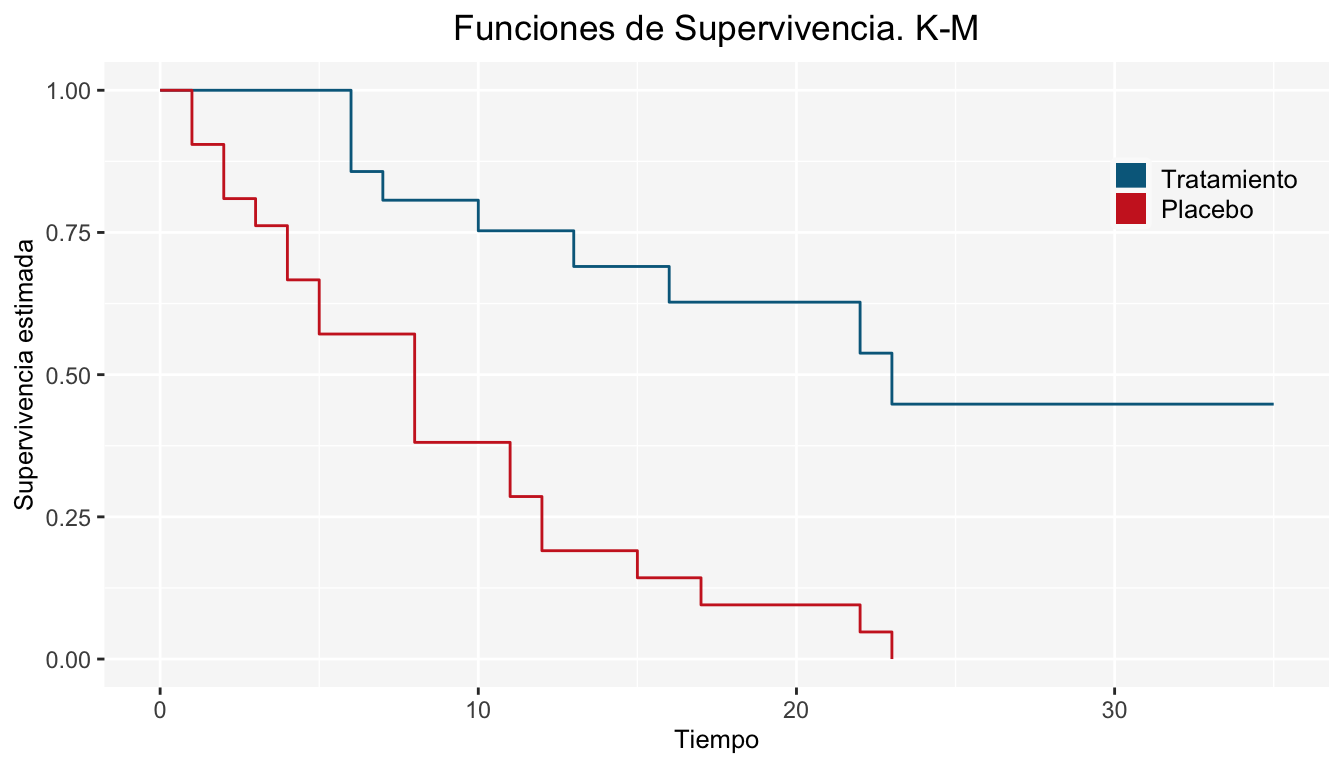
\includegraphics{_main_files/figure-latex/unnamed-chunk-35-1} \end{center}

Las funciones de supervivencia de los dos grupos ``parecen'' tener diferencia, de acuerdo a la gráfica anterior. No obstante, debemos comprobar si es una diferencia \emph{significativa}. Enseguida corroboraremos tal afirmación mediante la prueba Log-Rank.

La siguiente tabla muestra los individuos que fallan y los individuos en riesgo de cada grupo para cada tiempo \(t_i\) (\(i=1,2,...,k\)), donde \(k\)=17. Además, se muestran los cálculos de las fallas esperadas para la construcción del estadístico Log-Rank:

\begin{table}
\centering
\begin{tabular}{ccccccccccc}
\toprule
$i$ & $t_i$ & $d_{1i}$ & $d_{2i}$ & $n_{1i}$ & $n_{2i}$ & $e_{1i}$ & $e_{2i}$ & $d_{1i} - e_{1i}$ & $d_{2i} - e_{2i}$ & $V_{1i}$\\
\midrule
1 & 1 & 0 & 2 & 21 & 21 & 1 & 1 & -1 & 1 & 0.49\\
2 & 2 & 0 & 2 & 21 & 19 & 1.05 & 0.95 & -1.05 & 1.05 & 0.49\\
3 & 3 & 0 & 1 & 21 & 17 & 0.55 & 0.45 & -0.55 & 0.55 & 0.25\\
4 & 4 & 0 & 2 & 21 & 16 & 1.14 & 0.86 & -1.14 & 1.14 & 0.48\\
5 & 5 & 0 & 2 & 21 & 14 & 1.2 & 0.8 & -1.2 & 1.2 & 0.47\\
\addlinespace
6 & 6 & 3 & 0 & 21 & 12 & 1.91 & 1.09 & 1.09 & -1.09 & 0.65\\
7 & 7 & 1 & 0 & 17 & 12 & 0.59 & 0.41 & 0.41 & -0.41 & 0.24\\
8 & 8 & 0 & 4 & 16 & 12 & 2.29 & 1.71 & -2.29 & 2.29 & 0.87\\
9 & 10 & 1 & 0 & 15 & 8 & 0.65 & 0.35 & 0.35 & -0.35 & 0.23\\
10 & 11 & 0 & 2 & 13 & 8 & 1.24 & 0.76 & -1.24 & 1.24 & 0.45\\
\addlinespace
11 & 12 & 0 & 2 & 12 & 6 & 1.33 & 0.67 & -1.33 & 1.33 & 0.42\\
12 & 13 & 1 & 0 & 12 & 4 & 0.75 & 0.25 & 0.25 & -0.25 & 0.19\\
13 & 15 & 0 & 1 & 11 & 4 & 0.73 & 0.27 & -0.73 & 0.73 & 0.2\\
14 & 16 & 1 & 0 & 11 & 3 & 0.79 & 0.21 & 0.21 & -0.21 & 0.17\\
15 & 17 & 0 & 1 & 10 & 3 & 0.77 & 0.23 & -0.77 & 0.77 & 0.18\\
\addlinespace
16 & 22 & 1 & 1 & 7 & 2 & 1.56 & 0.44 & -0.56 & 0.56 & 0.3\\
17 & 23 & 1 & 1 & 6 & 1 & 1.71 & 0.29 & -0.71 & 0.71 & 0.2\\
 &  &  &  &  &  &  &  &  &  & \\
Total &  & 9 & 21 &  &  & 19.25 & 10.75 & -10.25 & 10.25 & 6.26\\
\bottomrule
\end{tabular}
\end{table}

Entonces el estadístico \textbf{Log-Rank} es:

\[
L^2=\frac{(\sum_{i = 1}^k(d_{1i}-e_{1i}))^2}{\sum_{i=1}^{k}V_{1i}}=\frac{(-10.25)^2}{6.26}=16.78
\]

Para \(\alpha=0.05\) tenemos que \(J_{0.95}=3.8414\) por lo que:

\[
L^2=16.78>J_{0.95}=3.8414
\]

Por lo tanto, \textbf{se rechaza} \(H_0\) y se concluye que \textbf{existe diferencia significativa} entre las funciones de supervivencia para el Grupo 1 (Tratamiento) y el Grupo 2 (Placebo).

\hypertarget{prueba-generalizada-wilcoxon}{%
\section{Prueba Generalizada Wilcoxon}\label{prueba-generalizada-wilcoxon}}

Se considera la hipótesis a probar:

\[
\begin{array}{lllll}
H_{0}:S_{1}(t) = S_{2}(t) & \forall t>0 & vs & H_{a}:S_{1}(t) \neq S_{2}(t) & \mbox{p.a } t>0\\
\end{array}
\]

La prueba \emph{generalizada de Wilcoxon} es una generalización de la prueba \emph{Log-Rank}; Wilcoxon añade una \textbf{ponderación} a las fallas \emph{observadas} menos las fallas \emph{esperadas}. El estadístico en el que se basa la prueba de Wilcoxon es:

\[
U_{w} = \sum_{i = 1}^k n_{i}(d_{1i}-e_{1i})
\]

Bajo la hipótesis nula \(H_0\) tenemos que \(\mathbb{E}(U_{w}) = 0\) y \(V_{w} = Var(U_{w}) = \sum_{i=1}^{k}n_{i}^2V_{1i}\). En consecuencia:

\[
W=\frac{U_w-\mathbb{E}(U_{w})}{\sqrt{V_{w}}}=\frac{\sum_{i = 1}^k n_{i}(d_{1i}-e_{1i})}{\sqrt{\sum_{i=1}^{k}n_{i}^2V_{1i}}} \sim N(0,1)
\]

\[
\Longrightarrow W^2= \frac{(\sum_{i = 1}^k n_{i}(d_{1i}-e_{1i}))^2}{\sum_{i=1}^{k}n_{i}^2V_{1i}} \sim \chi^2_{(1)}
\]

Entonces, la \textbf{estadística} que consideraremos para la prueba generalizada de \textbf{Wilcoxon} será:

\[
W^2= \frac{(\sum_{i = 1}^k n_{i}(d_{1i}-e_{1i}))^2}{\sum_{i=1}^{k}n_{i}^2V_{1i}}
\]

La \textbf{Regla de Decisión} es rechazar \(H_0\) al nivel de significancia \(\alpha\) si:

\[
W^2>J_{1-\alpha}
\]

Donde \(J_{1-\alpha}\) es el cuantil \(1-\alpha\) de una \(\chi^2_{(1)}\).

\hypertarget{ejercicio-2}{%
\subsubsection*{Ejercicio}\label{ejercicio-2}}


Realice la prueba generalizada de Wilcoxon de acuerdo a los datos del ejemplo de la sección anterior.

\hypertarget{comparaciuxf3n-de-m-poblaciones}{%
\section{\texorpdfstring{Comparación de \(m\) Poblaciones}{Comparación de m Poblaciones}}\label{comparaciuxf3n-de-m-poblaciones}}

Si deseamos comparar las funciones de supervivencia de \(m\) poblaciones planteamos la siguiente hipótesis:

\[
H_0:S_1(t) = S_2(t) = ... = S_m(t) \forall t \mbox{ vs } H_a:S_r(t)\neq S_s(t) \mbox{ p.a } r\neq s; r,s = 1,...,m
\]

Para realizar la prueba, denotemos \(d_{i}\) el vector de fallas al tiempo \(t_i\), \(i=1,...,k\) con vector de medias \(\mathbb{E}(d_i)\) y las entradas de la matriz de varianzas\footnote{Se tiene \(n_{1j}\) y \(n_{2j}\) ya que se esta asumiendo que todas las poblaciones tienen una misma distribución, por lo que se esperaría que la varianza fuera la misma que para la población 1.} y covarianzas de la siguiente manera:

\[
Var(d_{ji}) = \frac{n_{1i}\cdot n_{2i}\cdot d_i(n_i-d_i)}{n_i^2(n_i-1)}
\]

\[
Cov(d_{ji},...,d_{hi}) = \frac{-n_{ji}\cdot n_{hi}\cdot d_i(n_i-d_i)}{n_i^2(n_i-1)} \mbox{ , } j \neq h
\]

Donde \(j\) y \(h\) denota el Grupo e \(i\) es el tiempo. Ahora bien, sumando sobre los tiempos de falla \(t_i\):

\[
\underline{D} = \sum_{i = 1}^k\{\underline{d}_i - \mathbb{E}(d_i)\}
\]

\[
\underline{V} = \sum_{i=1}^kVar(\underline{d}_i)
\]

\textbf{Mantel-Haenszel} propone probar la hipótesis de \(m\) supervivencias iguales usando la forma cuadrática \(O = D^{t}V^{-1}D\), donde \(V^{-1}\) es la inversa generalizada de \(V\) que bajo \(H_0\) se distribuye \(\chi^2_{(m-1)}\).

\hypertarget{part-lleno-de-riesgos}{%
\part{Lleno de riesgos}\label{part-lleno-de-riesgos}}

\hypertarget{modelo-de-riesgos-proporcionales}{%
\chapter{Modelo de Riesgos Proporcionales}\label{modelo-de-riesgos-proporcionales}}

Cuando se desea comparar 2 o más grupos de tiempos-evento, si los grupos son ``similares'' entonces se les pueden aplicar los métodos no paramétricos vistos. Usualmente los individuos en los grupos tienen características adicionales que pueden afectar el resultado, por ejemplo, variables como: edad, género, nivel socioeconómico, consumo del alcohol, ritmo cardiaco, nivel de colesterol, etcétera.

Dichas variables pueden usarse como \textbf{covariables} (variables explicativas, factores de riesgo, variables independientes) en un modelo que explique la variable respuesta. Así, después de ajustar las covariables, la comparación de tiempos de supervivencia entre grupos deberá tener menos sesgo y ser más precisa que la simple comparación de tiempos de supervivencia.

Otro problema a resolver será predecir la distribución del tiempo de ocurrencia de cierto evento a partir de un conjunto de covariables.

Los datos estarán dados de la siguiente forma: \((t_i, \delta_i,x_i)\) con \(i = 1,...n\), donde:

\begin{itemize}
\tightlist
\item
  \(i\): individuos.
\item
  \(t_i\): tiempo de falla o censura.
\item
  \(\delta_i\): indicador de falla o censura.
\item
  \(x_i\): conjunto de covariables.
\end{itemize}

Nota:

\begin{itemize}
\tightlist
\item
  \(X_i =(X_{i1}, X_{i2}, ..., X_{ip})\); donde \(p\)= número de covariables.
\item
  \(X_i\) puede depender del tiempo, es decir, \(X_{ik}\) es una v.a que cambia en el tiempo (peso, colesterol, etc.).
\end{itemize}

Sea \(h_i(t|X_i)\) la función de riesgo al tiempo \(t\) del individuo \(i\) dadas las covariables \(X_i\) (vector de riesgo). El \textbf{modelo} propuesto por Cox (1972) es:

\[
h_i(t) = \varphi(X_i ;\theta)\cdot h_0(t)
\]
Donde:

\begin{itemize}
\tightlist
\item
  \(\theta=(\theta_1,..., \theta_p)\) es el vector de \(p\) parámetros asociados a las covariables (coeficientes de regresión).
\item
  \(\varphi(\cdot,\cdot)\) es la \emph{función liga} de las covariables con el tiempo t.
\item
  \(h_{0}(t)\) es la función de riesgo \emph{base}.
\end{itemize}

La función \(\varphi(\cdot,\cdot)\) debe satisfacer que \(\varphi(0,\theta) =1\), esto para que, en ausencia de covariables, se tenga que \(h_i(t) = h_0(t)\).

La forma más común de \(\varphi(X_i, \theta)\) es \(\varphi(X_i, \theta) = e^{X_i^{'} \theta}\) (Supone que \(X_i\) no tiene intercepto), entonces:

\[
h_i(t) = e^{X_i^{'} \theta}\cdot h_0(t)
\]

Si aplicamos \emph{logaritmo} tenemos que:

\[
\ln(h_i(t)) = X_i^{'}\theta + \ln(h_0(t))
\]

\begin{equation}
\Longrightarrow X_i^{'}\cdot\theta = ln \left({\frac{h_i(t)}{h_0(t)}}\right)
\label{eq:cox-covariables-linear}
\end{equation}

Es decir, el cociente de la función de riesgo del individuo \(i\) con respecto al riesgo base será igual a una forma lineal de las covariables.

El nombre de riesgos proporcionales se deriva del cociente de las funciones de riesgo de dos individuos:

\[
\frac{h_i(t)}{h_j(t)} = \frac{e^{X_i^{'} \theta}\cdot h_0(t)}{e^{X_j^{'} \theta} \cdot h_0(t)} = e^{(X_i-X_j)' \theta}
\]

A la expresión anterior se le conoce como \textbf{riesgo relativo} y es constante en el tiempo, cuyo valor depende simplemente de la diferencia entre valores de las covariables de los dos individuos\footnote{No hay dependencia con el tiempo.}.

Si \(X_{1i} = 1\) y \(X_{1j} = 0\), representan tratamiento y placebo respectivamente, y si todas las demás covariables se mantienen constantes, entonces \(e^{\theta_1}\) es el riesgo de que se presente la falla con el tratamiento relativo a que se presente la falla con el placebo.

\[\frac{h_i(t)}{h_j(t)} = e^{\theta_1}\]
Bajo el modelo de riesgos proporcionales, las funciones de supervivencia y densidad del individuo \(i\) son:
\[S_i(t)=\{S_0(t)\}^{exp(X_i'\theta)}\]
\[f_i(t)=e^{(X_i'\theta)}h_0(t)\{S_0(t)\}^{exp(X_i'\theta)}\]

donde \(S_0(t)=exp\{-H_0(t)\}\) es la función de supervivencia base y \(H_0(t)\) la función de riesgo acumulado base.
Una consecuencia del supuesto de proporcionalidad entre los riesgos de dos individuos \(i,j\) con covariables \(X_i,X_j\) es que las funciones de riesgo y supervivencia \textbf{no se intersectan}.

\begin{center}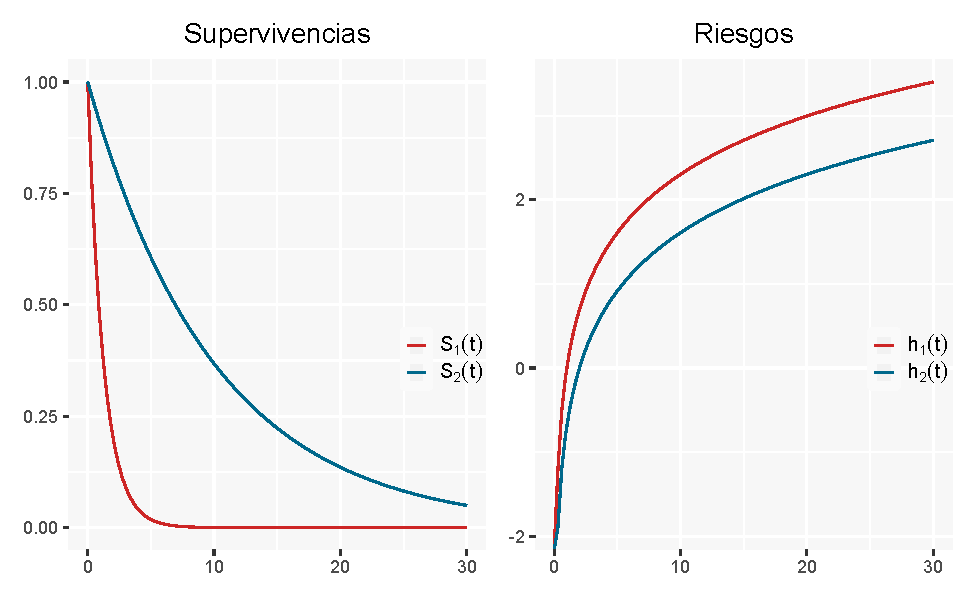
\includegraphics{_main_files/figure-latex/unnamed-chunk-37-1} \end{center}

\textbf{NOTA}: Si \(S_0(t)\) es miembro de una familia paramétrica, por lo general, \(S_i(t)\) no es miembro de la misma familia. Véase los siguientes ejemplos

\begin{itemize}
\item
  Riesgo base Weibull: \(h_0(t) = \lambda\alpha t^{\alpha-1}\)
  \[
  \begin{array}{cc}
  \implies h_i(t) = \lambda \alpha t^{\alpha-1}e^{X_i^{'}\theta} = \lambda e^{X_i^{'}\theta}\alpha t^{\alpha-1}&\therefore h_i\sim Weibull(\alpha, \lambda e^{X_i^{'}\theta})
  \end{array}
  \]
\item
  Riesgo base log-logistico: \(h_0(t) = \frac{\alpha \lambda t^{\alpha-1}}{(1+\lambda t^{\alpha})}\)
  \[
  \implies h_i(t) = \frac{e^{Xi^{'}\theta}\alpha t^{\alpha -1}}{(1+\lambda t^{\alpha})}
  \]
\item
  Riesgo base Gamma: \(S_0(t) = 1-lg(\lambda t, \beta)\)
  \[
  S_i(t) = \{S_0(t)\}^{e^{X_i^{'}\theta}} = \left(1-lg(\lambda t, \beta)\right)^{e^{X_i^{'}\theta}}
  \]
\end{itemize}

\hypertarget{inferencia-sobre-theta}{%
\section{\texorpdfstring{Inferencia sobre \(\theta\)}{Inferencia sobre \textbackslash theta}}\label{inferencia-sobre-theta}}

La inferencia para los modelos de riesgos proporcionales paramétricos se hacen por máxima verosimiliutd.

Sea \((t_i, \delta_i, X_i)\)

\begin{itemize}
\tightlist
\item
  i : individuos.
\item
  \(t_i\): tiempo de fallo o censura.
\item
  \(\delta_i\): Indicador de fallo o censura.
\item
  \(X_i\): Covariables.
\end{itemize}

Sean \(h_0(t|\alpha, \lambda)\) y \(S_0(t|\alpha, \lambda)\) funciones de riesgo y supervivencia base.

Entonces la función de verosimilitud para \((\theta, \alpha, \lambda)\) será:

\[
\begin{split}
\mathscr{L}(\theta, \alpha, \lambda) & =\prod_{i = 1}^{n}\{f_i(t)\}^{\delta_{i}}\{S_i(t)\}^{1-\delta_{i}}\\
 & =\prod_{i = 1}^{n}\left\{e^{X_i^{'}\theta}h_0(t)S_0(t)^{e^{X_i^{'}\theta}}\right\}^{\delta_{i}}\left\{S_0(t)^{e^{X_i^{'}\theta}}\right\}^{1-\delta_i}\\
 & =\prod_{i = 1}^{n}\left\{e^{X_i^{'}\theta}h_0(t)\}^{\delta_{i}}\{S_0(t)^{e^{X_i^{'}\theta}}\right\}
\end{split}
\]

\begin{itemize}
\tightlist
\item
  Los estimadores máximo verosímil se obtienen numéricamente.
\item
  La forma explicita de \(\mathscr{L}(\theta, \alpha, \lambda)\) dependerá de la elección de \(h_0\).
\item
  Inferencia para los parámetros más allá de la estimación puntual se basa en los resultados asintóticos.
\end{itemize}

\hypertarget{estimaciuxf3n-semiparamuxe9trica-verosimilitud-parcial.}{%
\section{Estimación Semiparamétrica (Verosimilitud parcial).}\label{estimaciuxf3n-semiparamuxe9trica-verosimilitud-parcial.}}

El modelo de riesgos proporcionales semiparamétrico surge cuando la función de riesgo base \(h_0(t)\) se considera como una parámetro desconocido, y en este caso es necesario hacer inferencia para \(\theta\) y \(h_0(t)\). El parámetro de interés más importante del modelo es \(\theta\) y entonces \(h_0(t)\) es considerado un parámetro de ruido.

Supongamos que los datos consisten en el vector de observaciones \(T = (T_1, ..., T_n)\) de la densidad \(f(t|\theta,\eta)\) donde \(\theta\) es el vector de parámetros de interés y \(\eta\) es parámetro de ruido.

Sean \(t_{(1)}<t_{(2)}<...<t_{(D)}\) los tiempos de fallo observados de manera exacta.

Sea \(X_{(j)}\) la variable asociada al individuo con tiempo de fallo \(t_{(j)}\).

Definimos \(R(t_{(j)})\) como el conjunto de todos los individuos en riesgo justo antes de \(t_{(j)}\).

Entonces la \textbf{verosimilitud parcial} para \(\theta\) es

\[
_p\mathscr{L}(\theta) = \prod_{j = 1}^{D}\frac{h_{j}(t_{(j)})}{\sum\limits_{i\in R(t_{(j)})}h_{i}(t_{(j)})} = \prod_{j = 1}^{D}\frac{\exp\left(X_{(j)}^{'}\theta\right)}{\sum\limits_{i\in R(t_{(j)})}\exp\left(X_{i}^{'}\theta\right)}
\]

OBS :

\begin{itemize}
\tightlist
\item
  \(_p\mathscr{L}(\theta)\) no depende de \(h_0(t)\)
\item
  El numerador depende sólo de la información del individuo que falla.
\item
  El denominador usa información de todos los individuos que aún no han experimentado fallo incluyendo censurados.
\item
  La verosimilitud parcial se trata como cualquier función de verosimilitud (aplica logaritmo, derivada igual a cero,\ldots)
\item
  \(\theta\) es un vector de dimensión \(p\implies\) se obtendrán \(p\) derivadas parciales. La mayoría de los paquetes usan algoritmos de Newton-Raphson para resolver el sistema de ecuaciones simultaneas.
\item
  Pruebas de hipótesis e intervalos de confianza para \(\theta\) se pueden obtener con distribución asintótica normal con media \(\theta\) y matriz de varianzas y covarianzas.
\end{itemize}

\hypertarget{estimador-de-breslow-h_0t-y-s_0t}{%
\section{\texorpdfstring{Estimador de Breslow (\(H_{0}(t)\) y \(S_{0}(t)\))}{Estimador de Breslow (H\_\{0\}(t) y S\_\{0\}(t))}}\label{estimador-de-breslow-h_0t-y-s_0t}}

Si la funciones base son también de interés, se puede utilizar el estimador propuesto por Berslow (1974) que es una generalización del estimador de \emph{Nelson-Aalen}.

\[\hat{H_{0}}(t) = \sum_{i:t_i\leq t}\left \{\frac{\delta_i}{\sum_{j = 1}^nY_j(t_i)e^{X_j^{'}\hat{\theta}}} \right \} = \frac{\mbox{Fallecidos}}{\mbox{Individuos en riesgo}}\]
donde \(Y_i(t) = \mathbb{1}_{\{t_i\geq t\}}\) indicadora si \(\hat{\theta} = 0\) y \(\hat{H_0}(t)\) es el estimador de Nelson-Aalen visto previamente.

\[\therefore \hat{S_0(t)}  = exp\{-\hat{H_0}(t)\} = e^{\sum_{i:t_i\leq t}\left \{\frac{\delta_i}{\sum_{j = 1}^nY_j(t_i)e^{X_j^{'}\hat{\theta}}} \right \}}\]

\textbf{Notas}

\begin{enumerate}
\def\labelenumi{\arabic{enumi}.}
\tightlist
\item
  En el caso de que se presenten \textbf{empates} (múltiples individuos con el mismo tiempo de fallo) la \(_p\mathscr{L}(\theta)\) debe ajustarse para que se considere la naturaleza discreta de las observaciones.
\item
  El modelo de riesgos proporcionales permite la incorporación de covariables dependientes en el tiempo.
\end{enumerate}

\hypertarget{ejemplo-1-2}{%
\subsubsection*{Ejemplo 1}\label{ejemplo-1-2}}


Un estudio sobre la supervivencia clasifica según la raza en: blanco, negro e hispano. Entonces las variable \(X_1\) toma los siguientes valores:

\[
\begin{array}{ll}
X_1 = \mbox{1 si es blanco } \\
X_1 = \mbox{2 si es negro } \\
X_1 = \mbox{3 si es hispano} \\
\end{array}
\]

Sin embrago, también podría plantearse como dos variables \(X_1\) y \(X_2\)
\[
\begin{array}{ll}
X_1 = 1 \mbox{ si es blanco, 0 en otro caso.}\\
X_2 = 1 \mbox{ si es negro, 0 en otro caso}\\
\end{array}
\]

Entonces, el modelo de riesgos proporcionales será: \(h(t|X) = h_0e^{\beta_1X_1+\beta_2X_2}\)

\begin{itemize}
\tightlist
\item
  Si \(h(t|X_1=1, X_2 = 0) = h_0(t)e^{\beta_1}\longrightarrow\) Riesgo de blanco
\item
  Si \(h(t|X_1=0, X_2 = 1) = h_0(t)e^{\beta_2}\longrightarrow\) Riesgo de negro
\item
  Si \(h(t|X_1=0, X_2 = 0) = h_0(t)\longrightarrow\) Riesgo de hispano (riesgo base)
\end{itemize}

Riesgos relativos:

\begin{itemize}
\tightlist
\item
  Entre negro e hispano: \(\frac{h(t|X_1 = 0, X_2 = 1)}{h(t|X_1 = 0, X_2 = 0)} = \frac{h_0(t)e^{\beta_2}}{h_{0}(t)}=e^{\beta_2}\)
\end{itemize}

Es decir, \(e^{\beta_2}\) son las veces que el riesgo que tienen los negros en comparación con los hispanos.

\begin{itemize}
\tightlist
\item
  Se busca que el riesgo relativo sea \(\neq1\) para poder decir que la categoría segmenta datos.
\end{itemize}

\hypertarget{ejemplo-2-2}{%
\subsubsection*{Ejemplo 2}\label{ejemplo-2-2}}


Un estudio con 863 pacientes con trasplante de hígado. Dos de las variable que se recabaron de los pacientes fueron, género y raza. Entonces los pacientes en el estudio se dividieron en las siguientes categorías

\[
\begin{array}{ll}
432 \mbox{ hombres blancos}\\
92 \mbox{ hombres negros}\\
286 \mbox{ mujeres blancas}\\
59 \mbox{ mujeres negras}\\
\end{array}
\]

Para ajustar un modelo de riesgos proporcionales a estos datos, una opción es definir 3 covariables:

\[
\begin{array}{ll}
Z_1 = 1 \mbox{ hombre negro, 0.e.o.c}\\
Z_2 = 1 \mbox{ hombre blanco, 0.e.o.c}\\
Z_3 = 1 \mbox{ mujer negra, 0.e.o.c}\\
\end{array}
\]
Y el modelo para la función de riesgo será:
\[h(t|Z) = h_0(t)exp \{ \theta_1Z_1 + \theta_2Z_2 + \theta_3Z_3\}\]

Los estimadores máximo verosímil son \(\hat{\theta_1} = 0.160\), \(\hat{\theta_2} = 0.298\), \(\hat{\theta_3} = 0.657\).

Riesgo relativo de hombre negro con mujer blanca :

\[h(t|Z) = \frac{h_0(t)exp\{0.160\}}{h_0(t)exp\{0\}} = e^{0.160} = 1.17\]
\(\therefore\) Los hombres negros son más propensos a morir por trasplante de hígado que las mujeres blancas; es decir, por cada mujer blanca, un hombre negro (1.17) muere en el trasplante.

En el caso de un hombre negro y un hombre blanco

\[h(t|Z) = \frac{h_0(t)exp\{0.160\}}{h_0(t)exp\{0.298\}} = e^{-0.088} = 0.9157609\]

Otra opción de plantear el modelo es con 2 covariables y una interacción, y quedaría de la siguiente forma:

\[
\begin{array}{ll}
Z_1 = 1 \mbox{ Si es mujer, 0  e.o.c}\\
Z_2 = 1 \mbox{ Si es negro(a), 0  e.o.c}\\
Z_3 = Z_1\cdot Z_2 \mbox{ Esta variable tomará el valor 1 si es mujer negra, y 0  e.o.c}
\end{array}
\]

Y el modelo para la función de riesgo será: \(h(t|Z) = h_0exp\{\theta_1Z_1+\theta_2Z_2+\theta_3Z_1Z_2\}\).

Los estimadores máximo verosímil son
\(\hat{\theta_1} = -.2484, \hat{\theta_2} =-.0888, \hat{\theta_3} = .7435\).
Hay que notar que la interpretación de las \(\theta's\) será diferente y en este caso el parámetro de interés será el de la interacción (\(\theta_3\))

Riesgos relativos :

\[\frac{\mbox{Hombre negro}}{\mbox{Mujer blanca}} = \frac{h_0(t)exp\{-0.0888\}}{h_0exp\{-0.2484\}} = e^{-(0.0888+0.2484)} = e^{-.1596} = 1.17\]

Véase que es el mismo resultado que se obtuvo en el modelo anterior, por lo que se sigue conservando el mismo riesgo independiente del modelo.

\textbf{Ejercicios}

\begin{enumerate}
\def\labelenumi{\arabic{enumi})}
\item
  Calcular el riesgo mujer negra relativo a mujer blanca.
\item
  Calcular el riesgo mujer negra relativo a hombre negro
\item
  Calcular el riesgo hombre blanco relativo a mujer blanca.
\end{enumerate}

\textbf{RECORDATORIO: Codificación de variables categóricas}.

Una variable categórica con k clases se transforma en \(k-1\) variables binarias.

\hypertarget{ejemplo-1-3}{%
\subsubsection*{Ejemplo 1}\label{ejemplo-1-3}}


X: Color de cabello \{negro, cafe, rojo, blanco\}. Tenemos una variable con 4 categorías. Por lo que la transformaremos en 3 variables binarias

\[
\begin{array}{l}
X_1 = \mbox{1 si es negro, 0 e.o.c } \\
X_2 = \mbox{1 si es café. 0 e.o.c } \\
X_3 = \mbox{1 si es rojo, 0.e.o.c} \\
\end{array}
\]

Con estas tres variables se cubren todas las opciones de color de cabello.

\hypertarget{significancia-de-los-paruxe1metros-prueba-de-wald}{%
\section{Significancia de los parámetros (Prueba de Wald)}\label{significancia-de-los-paruxe1metros-prueba-de-wald}}

¿Son significativos \(\hat{\theta_1}, \hat{\theta_2}, \hat{\theta_3}\) en ejemplo numero 2?

Similar al caso de regresión lineal, la significancia de los parámetros radica en la importancia del riesgo proporcionado por las covariables asociadas a parámetros. Y en caso de no ser significativos los parámetros, las covariables se podrían eliminar del modelo.

\textbf{Prueba de hipótesis:} Nos interesa hacer pruebas sobre \(\theta\), de manera general:

\[H_0:\theta_1 = \theta_{H_0}\mbox{ vs }H_1:\theta_1\neq \theta_{H_0}\]
donde \(\theta = (\theta_1^t, \theta_2^t) = (\theta_1, \theta_2, ..., \theta_p)\)

\begin{itemize}
\tightlist
\item
  \(\theta_1:\) Es el vector de \(q*1\) (\(q\) parámetros de interés)
\item
  \(\theta_2:\) Los parámetros restantes (\(p-q\))
\end{itemize}

Partimos la matriz de información : \(I = \begin{pmatrix}I_{11} & I_{12} \\ I_{21} & I_{22}\end{pmatrix}\)

Donde \(I_{11}\), \(I_{22}\) segundas derivadas de la función de verosimilitud.

La \textbf{Prueba de Wald} se define como:

\[
X_w^2 =(\hat{\theta_1}-\hat{\theta_{H_0}})^{'}[I^{*}(\theta)]^{-1}(\hat{\theta_1}-\hat{\theta_{H_0}})
\]

Donde \(I^{*}(\theta)\) es la matriz \(q*q\) superior de \(I\).

\begin{itemize}
\item
  Para muestras grandes, la estadística de prueba: \(X_w^2\sim\chi_{(q)}^2\)
\item
  Un criterio de información es el proporcionado por el criterio de Aikaike (\(ACI\)):
\end{itemize}

\[AIC  = -2log{\mathscr{L}}+kp\]

\begin{itemize}
\tightlist
\item
  \(\mathscr{L}\): Función de verosimilitud.
\item
  \(k\): Cte.(usualmente igual a 2).
\item
  \(p\): \# de parámetros en el modelo.
\end{itemize}

Para la construcción del modelo usando el modelo de riesgos proporcionales de Cox, se puede usar el estadístico de Wald para seleccionar covariables significativas\footnote{Recordar que por la ecuación \eqref{eq:cox-covariables-linear}, el modelo esta asumiendo una forma lineal de las covariables.} y considerando el valor del AIC para evaluar la mejora en el modelo\footnote{Para un mayor número de variables el \(AIC\uparrow\) pero para variables más significativas \(AIC\downarrow\).}.

\hypertarget{estimaciuxf3n-de-st-despuuxe9s-de-obtener-las-estimaciones-de-los-paruxe1metros-del-modelo-de-cox}{%
\section{\texorpdfstring{Estimación de \(S(t)\) después de obtener las estimaciones de los parámetros del modelo de Cox}{Estimación de S(t) después de obtener las estimaciones de los parámetros del modelo de Cox}}\label{estimaciuxf3n-de-st-despuuxe9s-de-obtener-las-estimaciones-de-los-paruxe1metros-del-modelo-de-cox}}

Hasta el momento se han dado estimadores para \(\theta\) y pruebas sobre dicho parámetro; es decir, teniendo el modelo de riesgos proporcionales \(h(t|X) = h_0(t)e^{X^{'}\theta}\) y ajustando dicho modelo a nuestros datos obtenemos \(\hat{\theta}\). Ahora lo que se desea es la función de supervivencia con el conjunto de covariables \(X_i\).Para ello sea \(t_1<t_2, \dots<t_D\) todos los tiempos de falla y \(d_i\) el número de fallas del tiempo \(t_i\). Entonces

\[
\omega(t_i, \hat{\theta}) = \sum_{j\in R(t_i)}\exp\left\{\sum_{h=1}^D\hat{\theta}_hX_{jh}\right\}
\]

Y el estimador de la función de riesgo acumulado base será la siguiente, la cual es una función escalonada a cada tiempo de falla.

\[
\hat{H_0}(t) = \sum_{t_i\leq t}\frac{d_i}{w(t_i, \hat{\theta})}
\]

Por lo que un estimador de la función de supervivencia base será el siguiente, el cual corresponde a los individuos cuyas covariables \(X\) son ceros.

\[
\hat{S}_0(t) = \exp\{-\hat{H}_0(t)\}
\]

Para estimar la función de supervivencia para un individuo con covariables \(X^{*}\) se utilizará el siguiente estimador

\[
\hat{S}(t|X^{*})=\hat{S}_0(t)\exp\left\{\hat{\theta^{'}}X^{*}\right\}
\]
La siguiente gráfica es un ejemplo comparativo de dos estimaciones de funciones de supervivencia, una con el método de Kaplan-Meier y Cox.

\begin{center}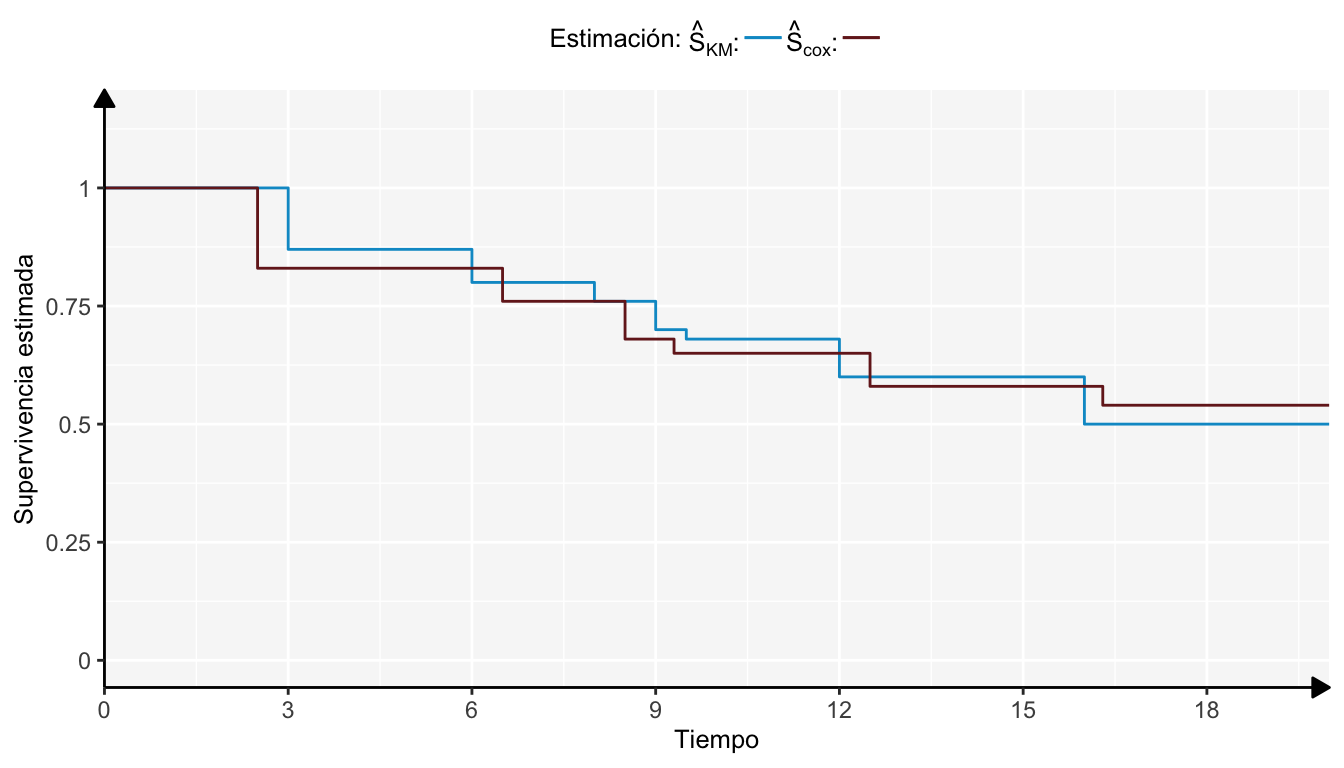
\includegraphics{_main_files/figure-latex/unnamed-chunk-38-1} \end{center}

\hypertarget{verificaciuxf3n-de-ajuste-de-modelo}{%
\section{Verificación de ajuste de Modelo}\label{verificaciuxf3n-de-ajuste-de-modelo}}

Mediante gráficos de las funciones de supervivencia buscamos las funciones de supervivencia para los distintos valores de \(X\)'s donde \textbf{no} se crucen\footnote{Por el hecho de que se busca \textbf{proporcionalidad} y, por lo tanto, que la segregación separe completamente a la población.}.

En caso de que el modelo de Cox no cumpla con el supuesto de proporcionalidad se puede corregir el modelo mediante:

\begin{enumerate}
\def\labelenumi{\arabic{enumi})}
\item
  Agregar más covariables
\item
  Considerar interacciones entre las covariables
\item
  Introducir términos no lineales
\item
  Permitir que las covariables dependan del tiempo
\end{enumerate}

\hypertarget{extensiuxf3n-del-modelo-de-cox-a-covariables-dependientes-del-tiempo}{%
\section{Extensión del modelo de Cox a covariables dependientes del tiempo}\label{extensiuxf3n-del-modelo-de-cox-a-covariables-dependientes-del-tiempo}}

Sea \(X(t)=[X_1(t),...,X_p(t)]\) es el conjunto de covariables o factores de riesgo al tiempo \(t\) que podrían afectar la distribución de la variable de supervivencia.

Entonces \(X_k(t)\)´s son covariables dependientes del tiempo cuyos valores cambian o permanecen constantes (como el caso anterior). Supondremos que los valores de estas covariables son predecibles (el valor es conocido).

Ejemplos de este tipo de variables son presión arterial, colesterol, tamaño del tumor, etc.

Sustituyendo en el modelo de Cox tenemos:

\[
\begin{split}
h(t|X(t))=&h_0 (t)\cdot exp\{\beta^`\cdot Z(t )\}\\
=&h_0(t) \cdot exp \left\{ \sum_{k=1}^{p} \beta_k \cdot Z(t)  \right\}
\end{split}
\]

Entonces para probar el supuesto de riesgos proporcionales se crea una variable artificial:

\[
X_2(t)= X_1 \cdot g(t) 
\]

donde \(X_1\) es una variable fija en el tiempo \(g(t)\) es una función que depende del tiempo usualmente

\[
g(t)= ln (t ) 
\]
y se ajusta un modelo de Cox para las covariables \(X_1\) y \(X_2(t)\), tenemos

\[  
\begin{split}
h(t|X(t)) &= h_0 \cdot exp \{ \beta_1 X_1 +\beta_2X_2(t) \}\\
&=h_0(t) \cdot exp \{ \beta_1 X_1+\beta_2 X_1\cdot g(t) \}
\end{split}
\]
y se realiza la prueba de hipótesis para \(\beta_2=0\). Si se desea evaluar riesgos proporcionales para 2 individuos con diferentes valores de \(X_1\)

\[
\frac{h(t|X_1)}{h(t|X_1^*)}= exp \{ \beta_1 (X_1-X_1^*)+\beta_2\cdot g(t)(X_1-X_1^*) \}
\]

la cuál dependerá del tiempo si \(\beta_2 \ne 0\).

  \bibliography{book.bib,packages.bib}

\end{document}
